
\chapter{Tri-dexel method}
\label{ch:tri_dexel}

The second discussed method to extract a triangulated surface from the VML's data model is based on a tri-dexel representation, \cf section \ref{sec:surface_representations}.
As observed with the previously shown method in chapter \ref{ch:direct_intersection}, reconstructing a surface directly form the many intersecting triangles stored in the VML's grid is computationally expensive, highly numerically unstable and prone to errors.
A more robust approach is desirable, which is able to always successfully reconstruct a surface with good quality.
This reconstruction should succeed independently of the complexity of the maintained geometry.
As a trade-off for this robustness, the approach may sacrifice surface exactness and filigree features.
Dexel-based representations fit this purpose nicely.
They provide a good abstraction of a machined workpiece with rich semantics.
The used grid resolution supplies an easy to configure level of detail and steering parameter between representation quality and memory/CPU demands.
Creating dexel-based representations from the VML's data model is achieved using an adaption of the already implemented, well-working and robust raycasting subsystem used for visualization, \cf section \ref{sec:raycasting}.
To achieve a good portrayal, independently of the workpiece's orientation, three axis-aligned dexel images will be generated, thus creating a tri-dexel representation.
For converting such a tri-dexel model into a final triangle mesh, various algorithms are found in literature.
An excellent example is Ren \etal's "Feature Conservation and Conversion of Tri-dexel Volumetric Models to Polyhedral Surface Models for Product Prototyping" \cite{tridexel_reconstruction}.
Their approach form the idea and foundation of the implementation presented in this chapter.


\section{Concept}
\label{sec:tri_dexel_concept}

Firstly, a tri-dexel representation of the VML's data model has to be obtained.
Dexel images, in general, are created by sampling the workpiece's surface along parallel lines.
This sampling process is already implemented in the raycasting subsystem as part of the visualization.
However, when sampling dexels, a ray must not stop at the first surface intersection, but continue through the whole data model and collect all intersections along its path.
At each intersection, the intersection depth, \ie distance from the ray's origin, and the surface normal of the intersected triangle is recorded as a dexel node.
From the dexel's origin and a node's depth the intersection point may be calculated.
The raycast itself is performed with axis-parallel rays starting at equidistant origins from three sides of the VML's data model, thus creating three dexel images.
Combining these dexel images creates a uniform regular grid, the tri-dexel grid.
Figure \ref{fig:cylinder_head_dexel} shows the cylinder head scene with a low-resolution dexel image and the final reconstruction.

\begin{figure}
	\centering
	\begin{subfigure}[t]{0.3\textwidth}
		\centering
		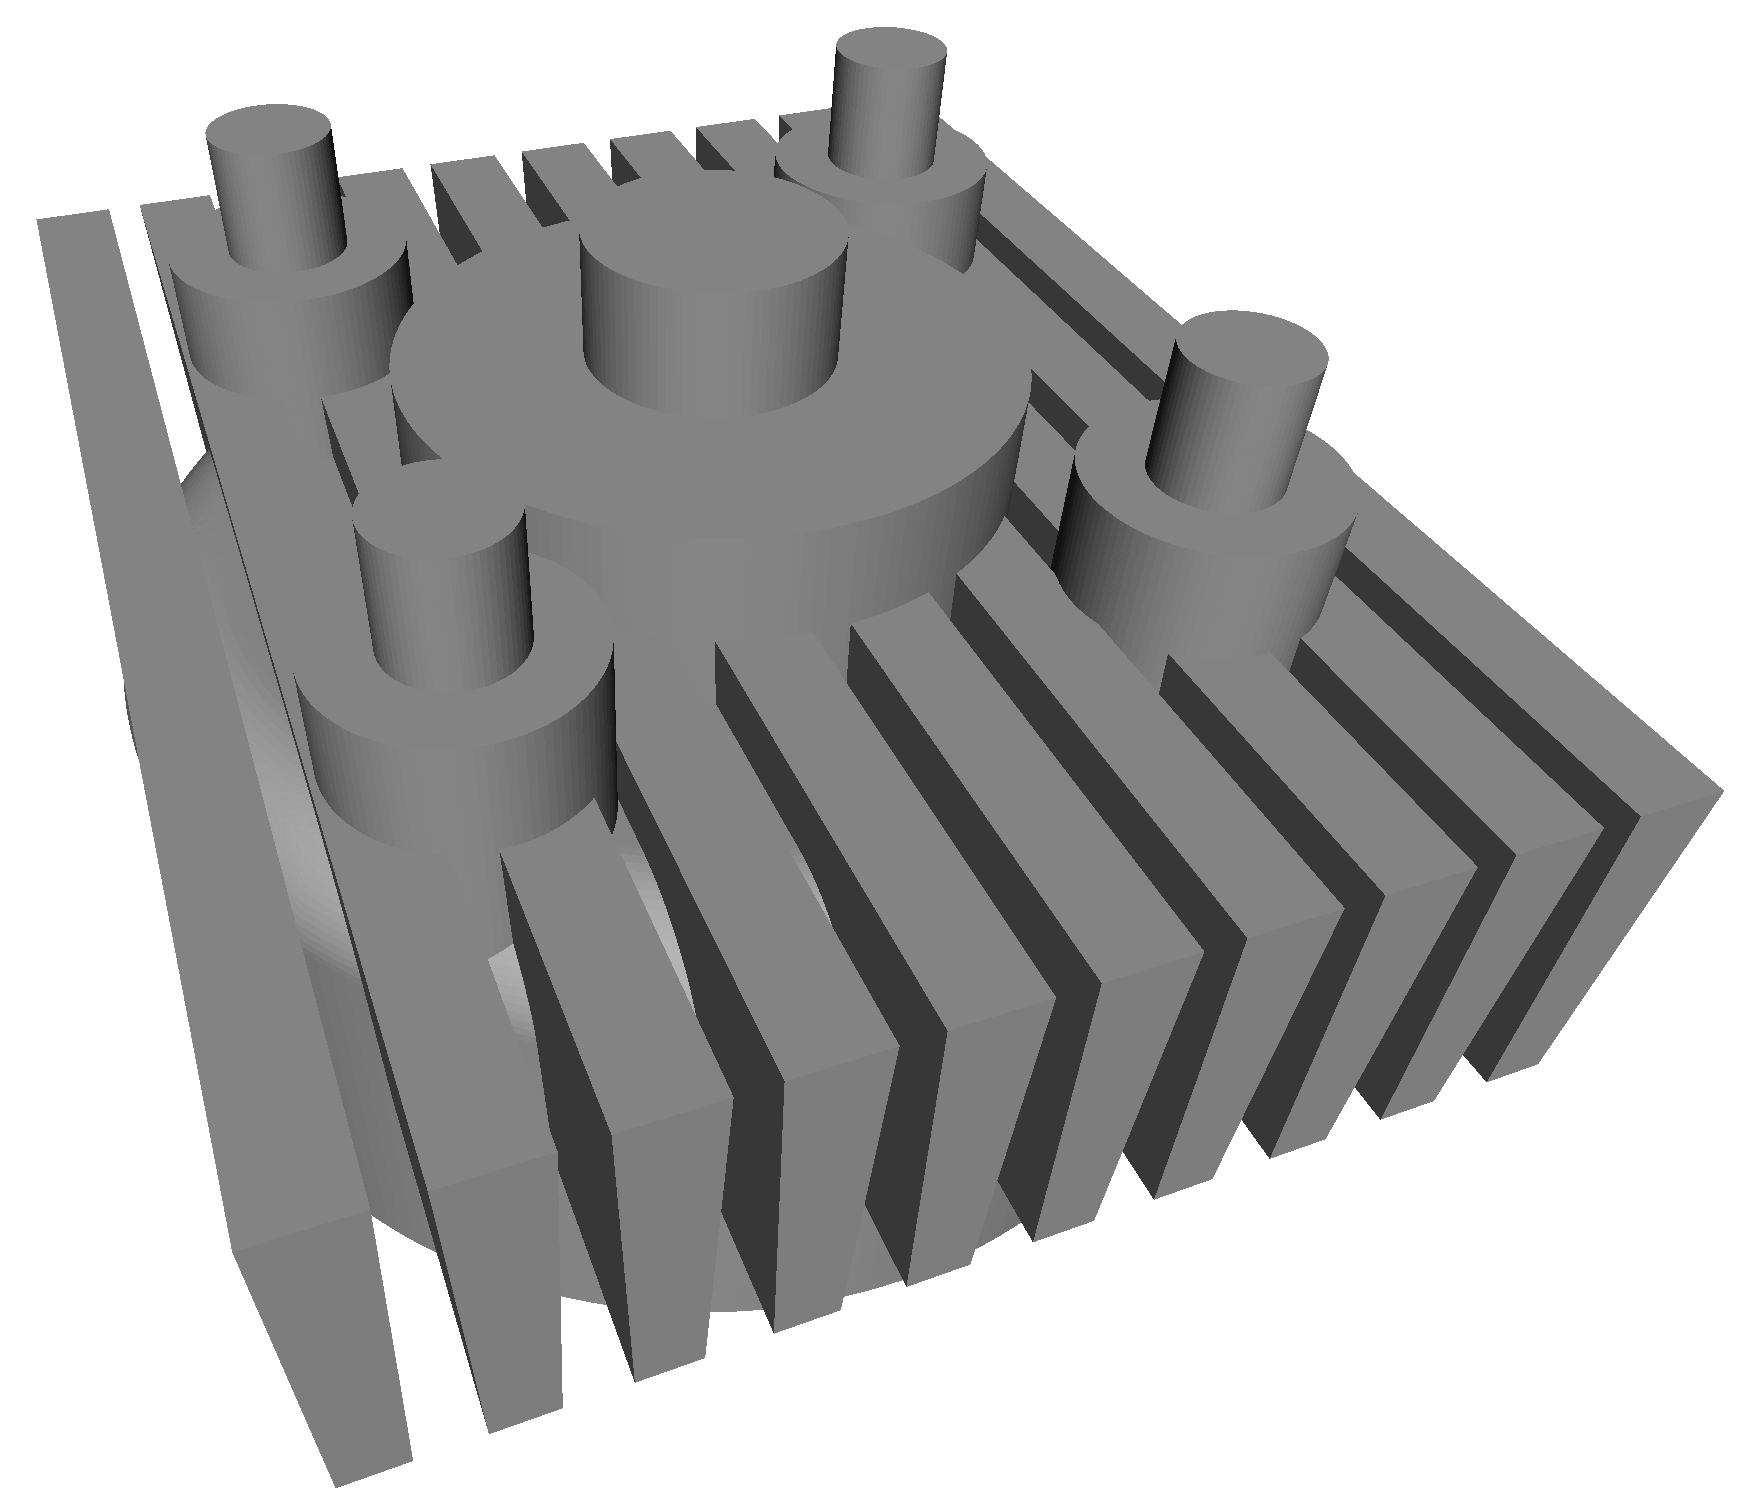
\includegraphics[width=\textwidth]{images/cylinder_head_stock_and_svs}
		\caption{Stock and SVs}
		\label{fig:cylinder_head_stock_sv}
	\end{subfigure}
	\begin{subfigure}[t]{0.3\textwidth}
		\centering
		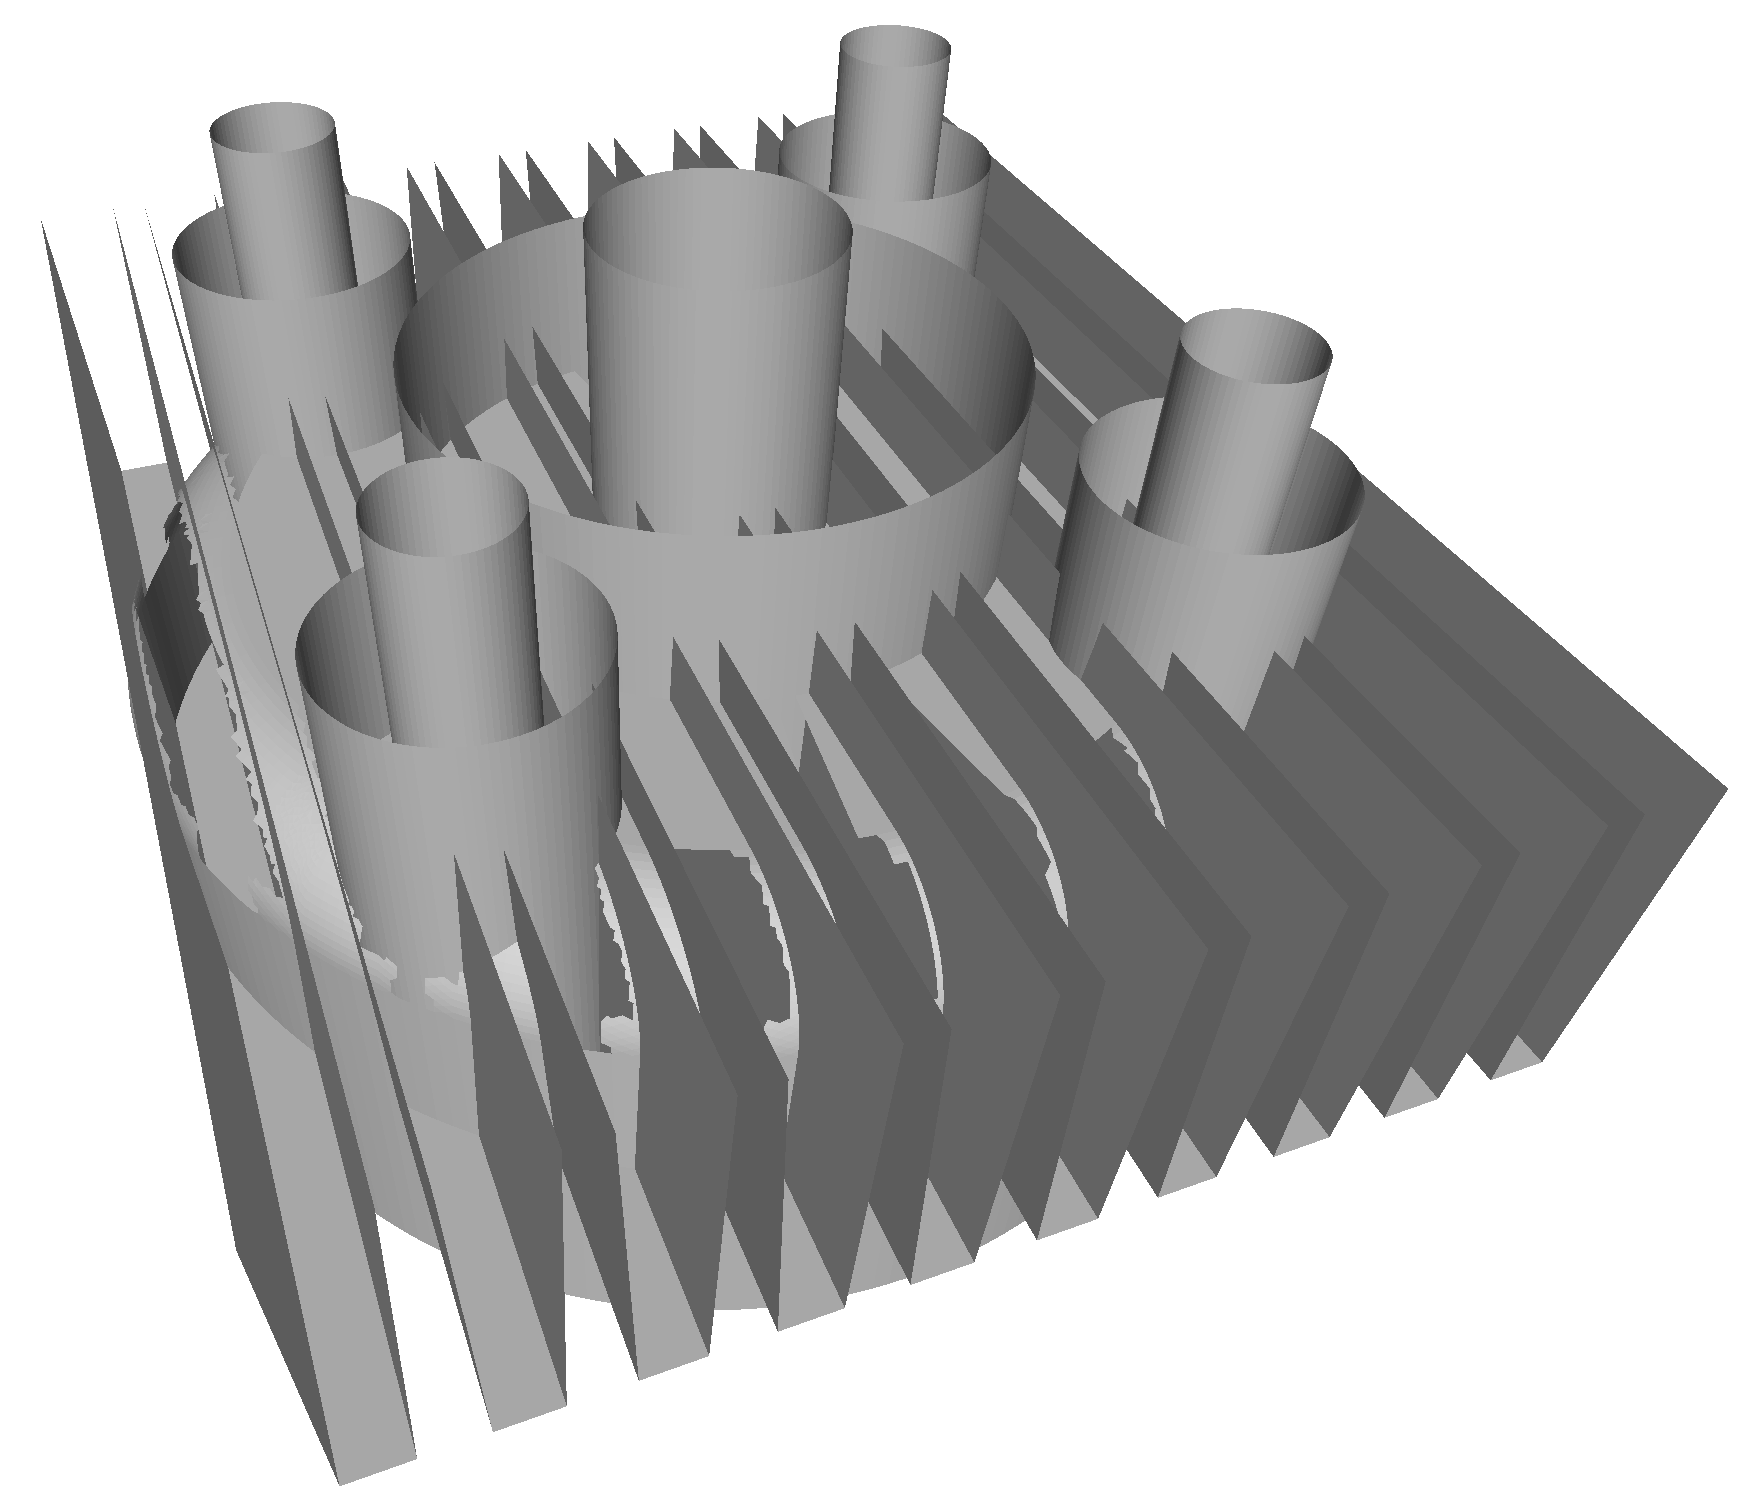
\includegraphics[width=\textwidth]{images/cylinder_head_vml}
		\caption{VML}
		\label{fig:cylinder_head_classified}
	\end{subfigure}
	\begin{subfigure}[t]{0.3\textwidth}
		\centering
		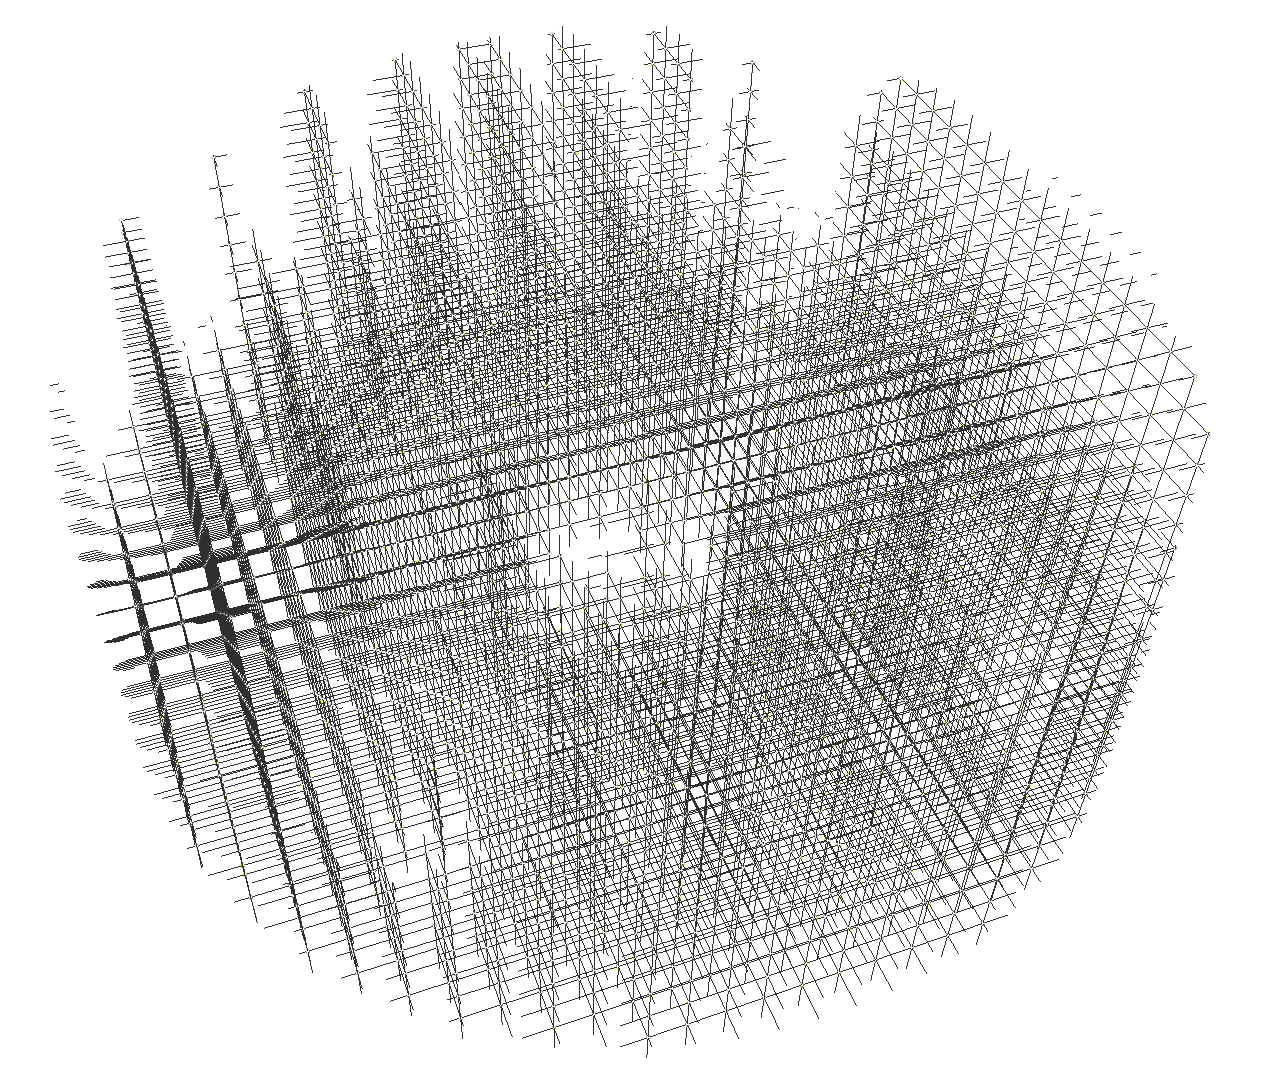
\includegraphics[width=\textwidth]{images/cylinder_head_dexel_image}
		\caption{Tri-dexel image}
		\label{fig:cylinder_head_dexel_image}
	\end{subfigure}
	\begin{subfigure}[t]{0.3\textwidth}
		\centering
		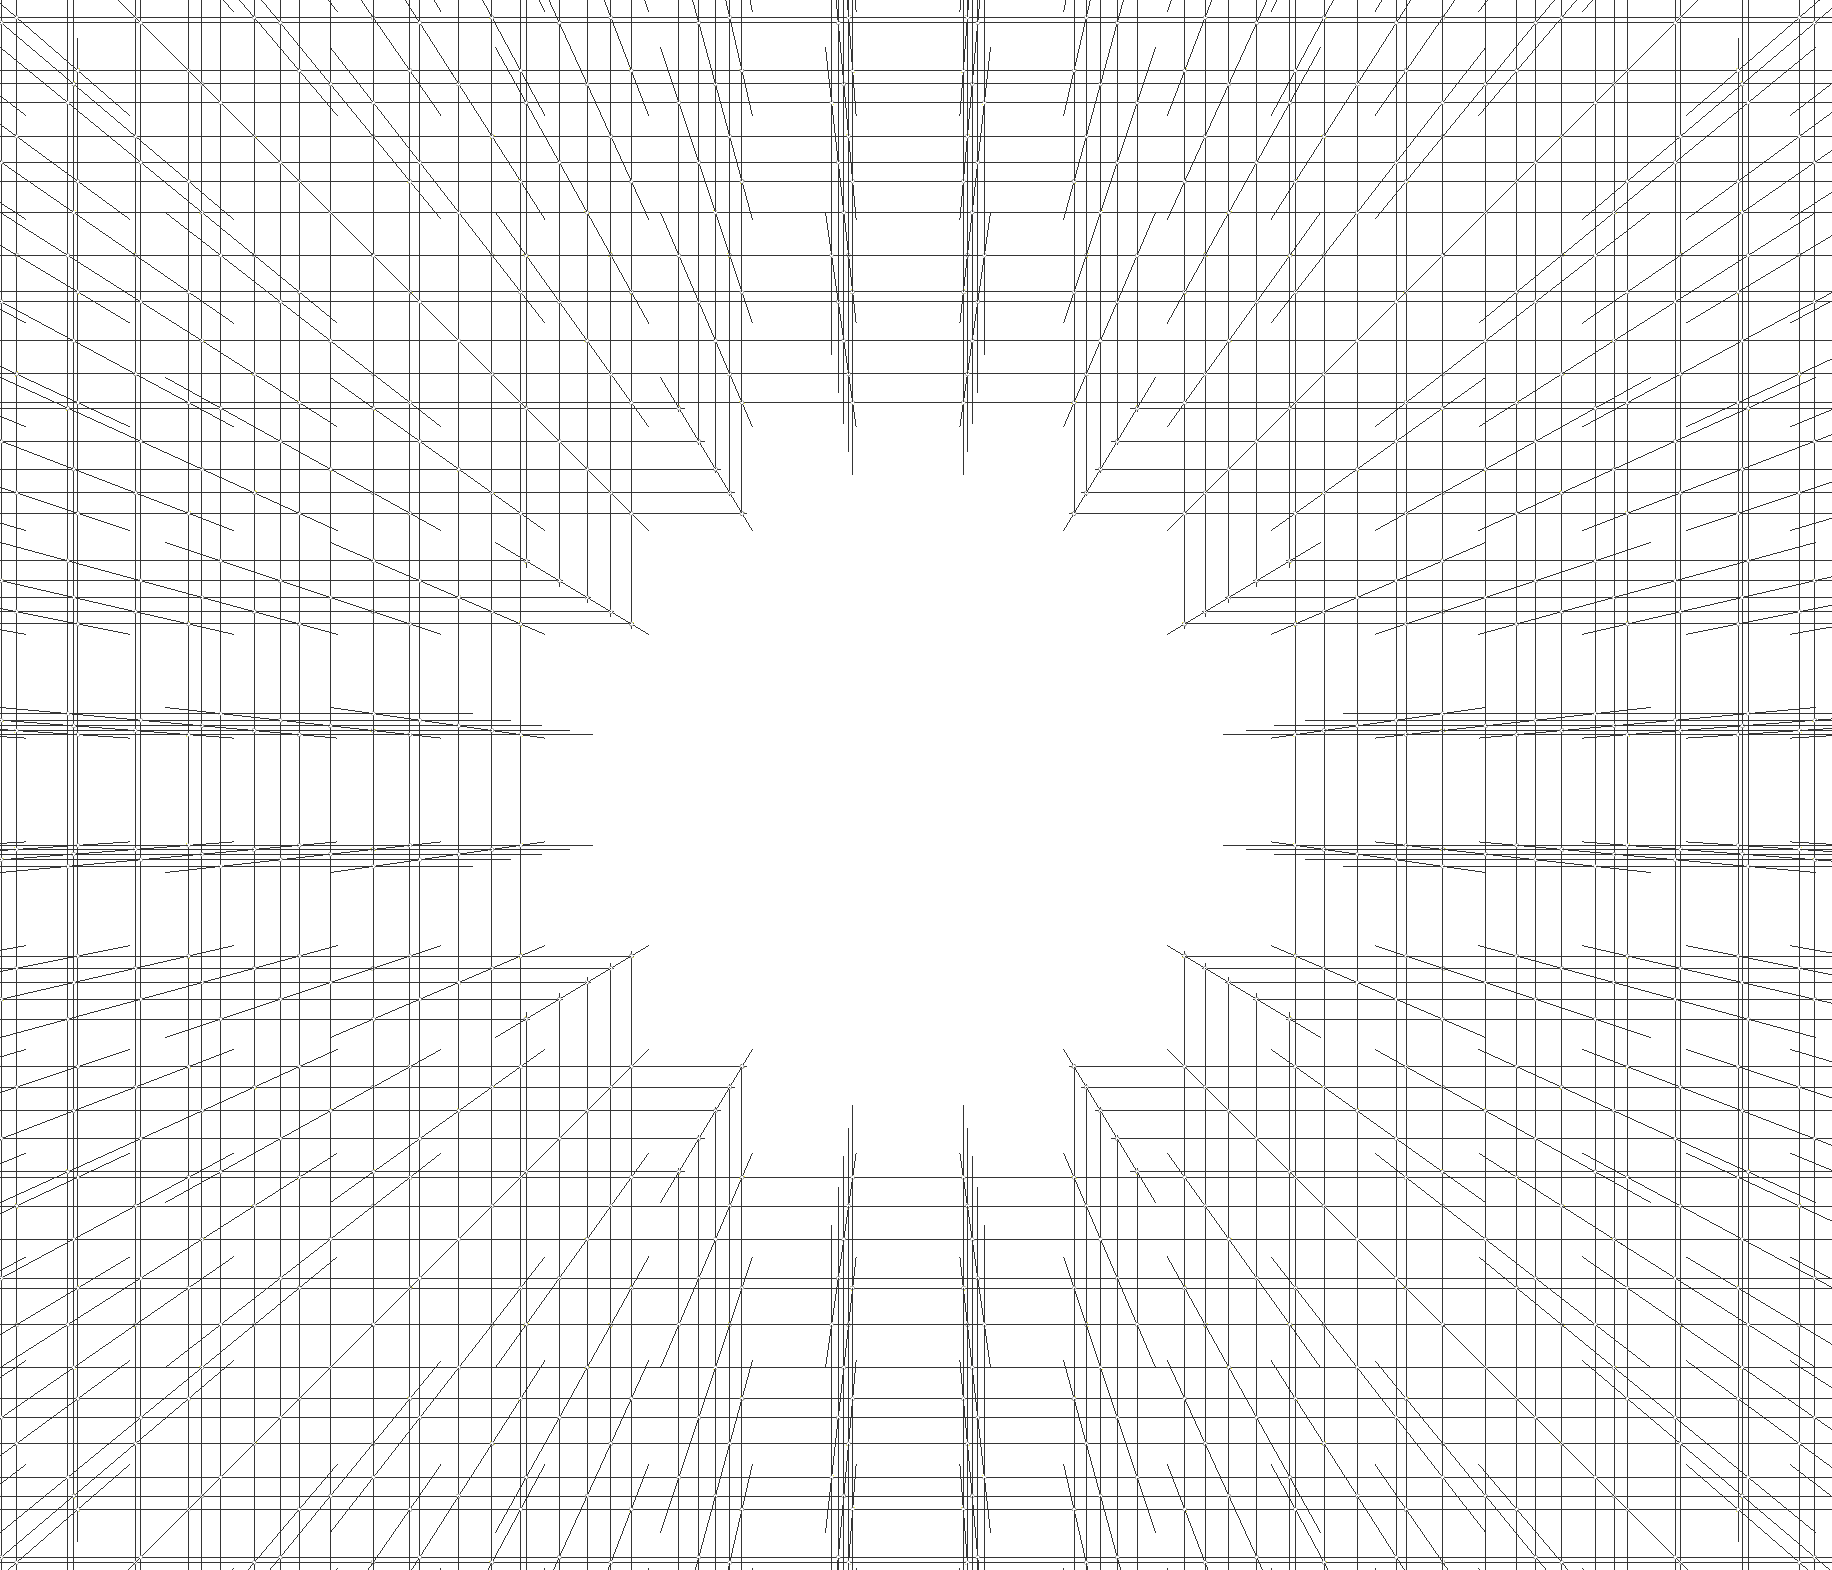
\includegraphics[width=\textwidth]{images/cylinder_head_dexel_image_center}
		\caption{Tri-dexel image center}
		\label{fig:cylinder_head_dexel_image_center}
	\end{subfigure}
	\begin{subfigure}[t]{0.3\textwidth}
		\centering
		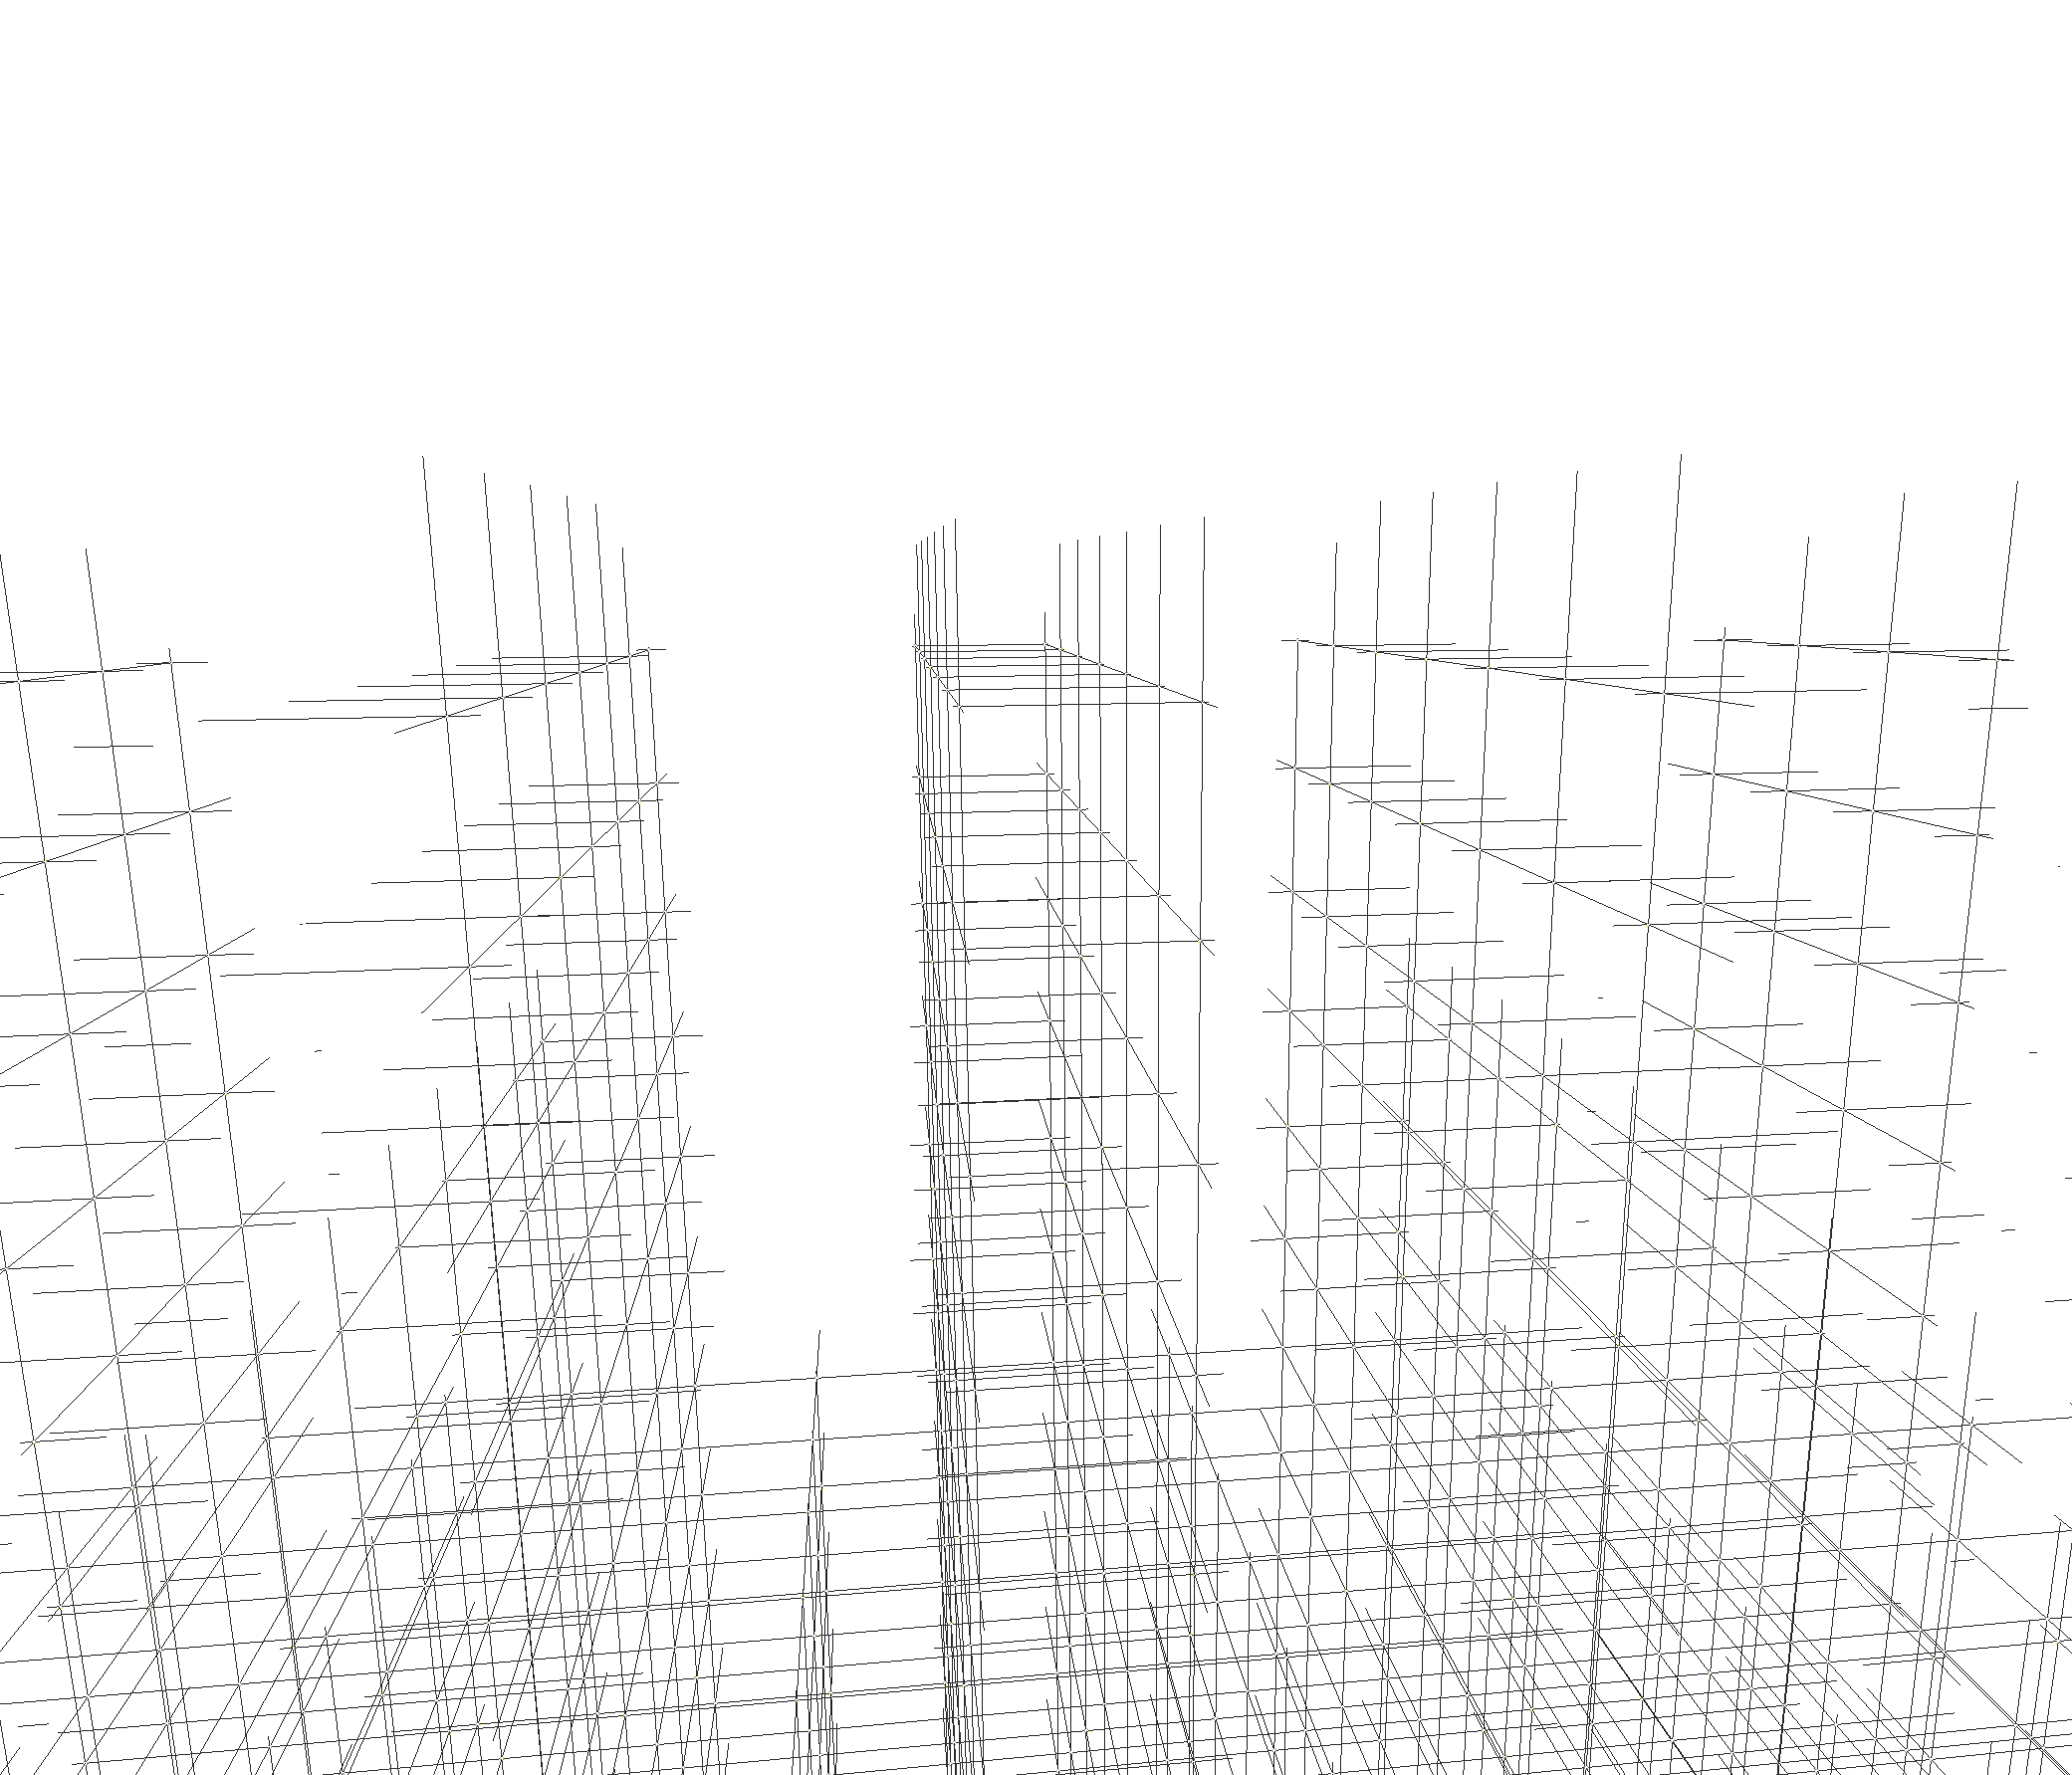
\includegraphics[width=\textwidth]{images/cylinder_head_dexel_image_fins}
		\caption{Tri-dexel image fins}
		\label{fig:cylinder_head_dexel_image_fins}
	\end{subfigure}
	\begin{subfigure}[t]{0.3\textwidth}
		\centering
		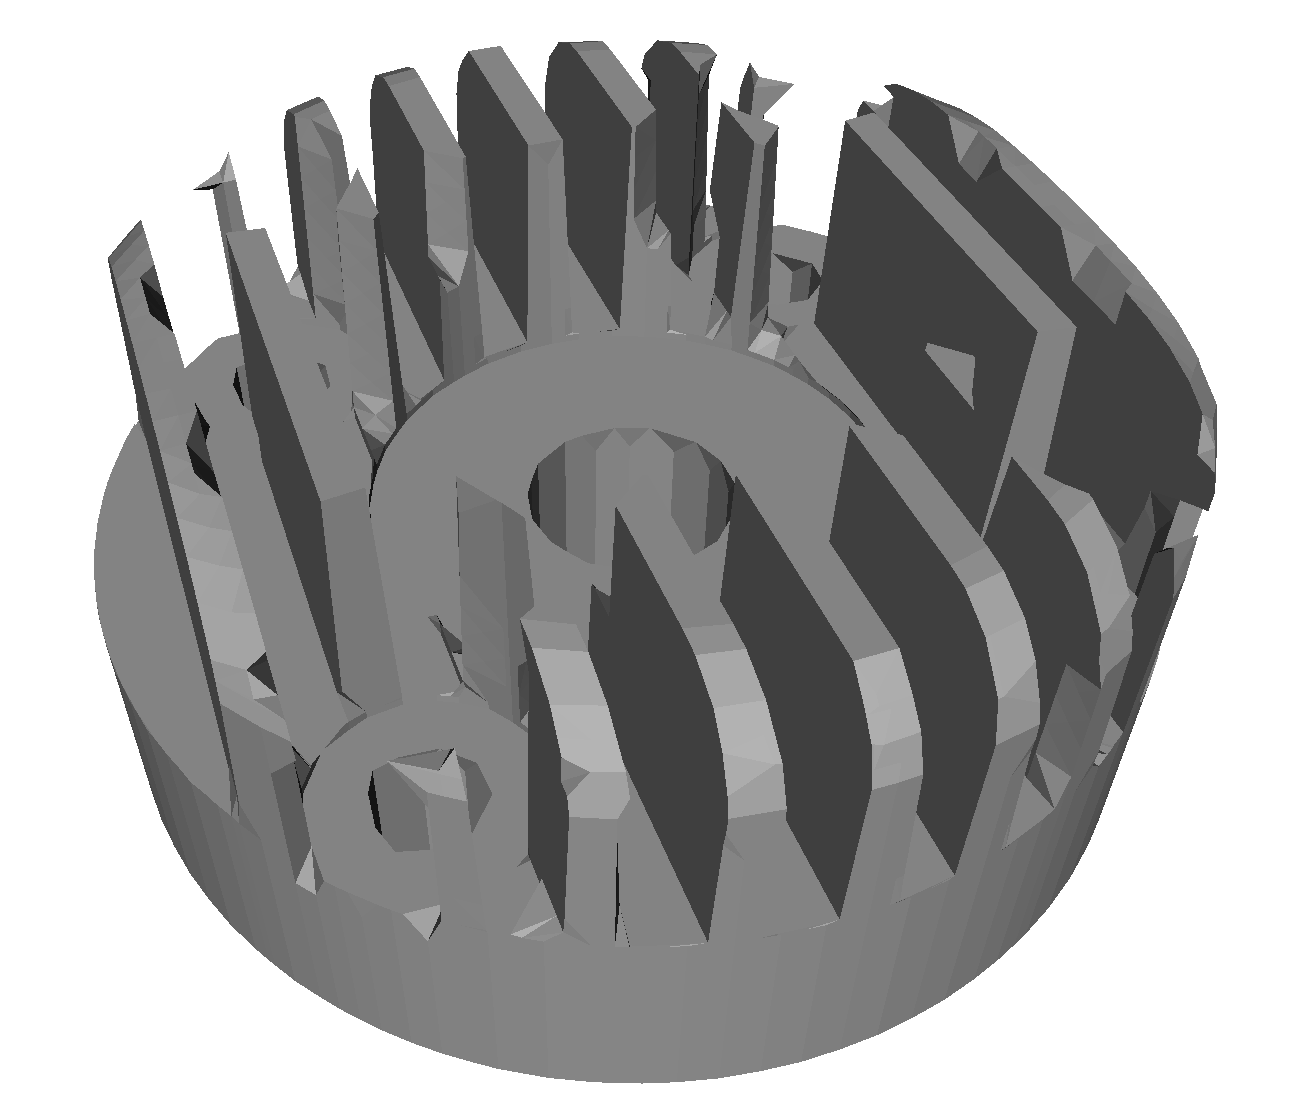
\includegraphics[width=\textwidth]{images/cylinder_head_reconstructed}
		\caption{Result}
		\label{fig:cylinder_head_reconstructed}
	\end{subfigure}
	\caption{
		Tri-dexel based surface reconstruction from the VML's data model of a cylinder head.
		Figure \subref{fig:cylinder_head_stock_sv} shows the stock and a few swept volumes creating the fins and drillings.
		Figure \subref{fig:cylinder_head_classified} shows the classification result after these solids have been mapped into the VML's regular grid.
		The removed triangles are clearly visible, especially at the swept volumes.
		By using a raycast of axis-parallel rays along all three coordinate system axes a tri-dexel representation is created as shown in figure \subref{fig:cylinder_head_dexel_image}.
		The resolution of the grid spawning the rays is 30 along the longest dimension.
		Figure \subref{fig:cylinder_head_dexel_image_center} and \subref{fig:cylinder_head_dexel_image_fins} show details of the tri-dexel image, the drilling at the center from above and the cylinder head's fins from the center.
		Finally, the reconstructed surface is shown in figure \subref{fig:cylinder_head_reconstructed}.
		Note the imperfections at the fin's edges and bases.
	}
	\label{fig:cylinder_head_dexel}
\end{figure}

Secondly, the tri-dexel representation is converted into a triangle mesh.
This procedure is mostly based on the paper mentioned in the introduction \cite{tridexel_reconstruction}.
Each intersection point of three orthogonal dexels from the tri-dexel grid forms a grid point.
If a grid point lies within a dexel segment on any of these dexels, it is said to be occupied, \ie lies within the workpiece's volume.
8 grid points and their 12 connecting edges along with their dexel segments are grouped into cells of the grid.
Each grid cell is then processed independently.
Figure \ref{fig:tri_dexel_cell} shows the structure of a tri-dexel cell.
%
\begin{figure}
	\centering
	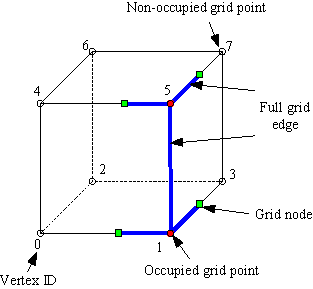
\includegraphics[width=0.5\textwidth]{images/tri_dexel_cell}
	\caption{
		A cell of a tri-dexel grid \cite{tridexel_reconstruction}.
		Occupied grid points are drawn in red, dexel nodes in green, dexel segments in blue.
		Each grid point is referenced using a number between 0 and 7.
	}
	\label{fig:tri_dexel_cell}
\end{figure}
%
Before a cell is triangulated, a few consistency checks and corrections are applied to the cell.
This process is called regularization and ensures a successful triangulation into a water-tight mesh.
Afterwards, the cell is triangulated.
For this purpose, a depth-first search process is iteratively started at non-occupied grid points of the cell to discover boundary loops.
Basically, the found loops may be triangulated right away to obtain a water tight mesh.
However, the quality of the triangulation may be further enhanced by taking normal information at the dexel nodes into account.
This is especially necessary to reconstruct features of the model.
This optional feature reconstruction pass is run on the loops found in the previous step and may create additional vertices.

\section{Implementation}
\label{sec:tri_dexel_implementation}

In order to run the tri-dexel surface reconstruction, the user must supply a resolution as parameter.
This resolution determines the size of the raycasted dexel images as well as the resulting tri-dexel grid.
For esthetic reasons, the specified resolution is only used for the longest dimension of the workpiece.
The resolution along the other dimensions is usually smaller in order to make the cells more cubic, although the implementation does not require cubic cells.
This property will become important in an extension to the tri-dexel reconstruction discussed in section \ref{sec:tri_dexel_cellslicing}.


In addition to the types already specified by the VML, \cf figure \ref{fig:vml_datamodel}, the tri-dexel reconstruction algorithm requires a few more types.
Most of these type definitions and also the algorithms themselves are vastly simplified when compared with the underlying source code.
Especially parallelism, asynchrony, memory efficient handling of data structures and numeric stability enhancements have been intentionally left out in the discussed pseudo code.


The additional types needed for the tri-dexel implementation are shown in the class diagram in figure \ref{fig:tri_dexel_datamodel}.
%
\begin{figure}
	\centering
	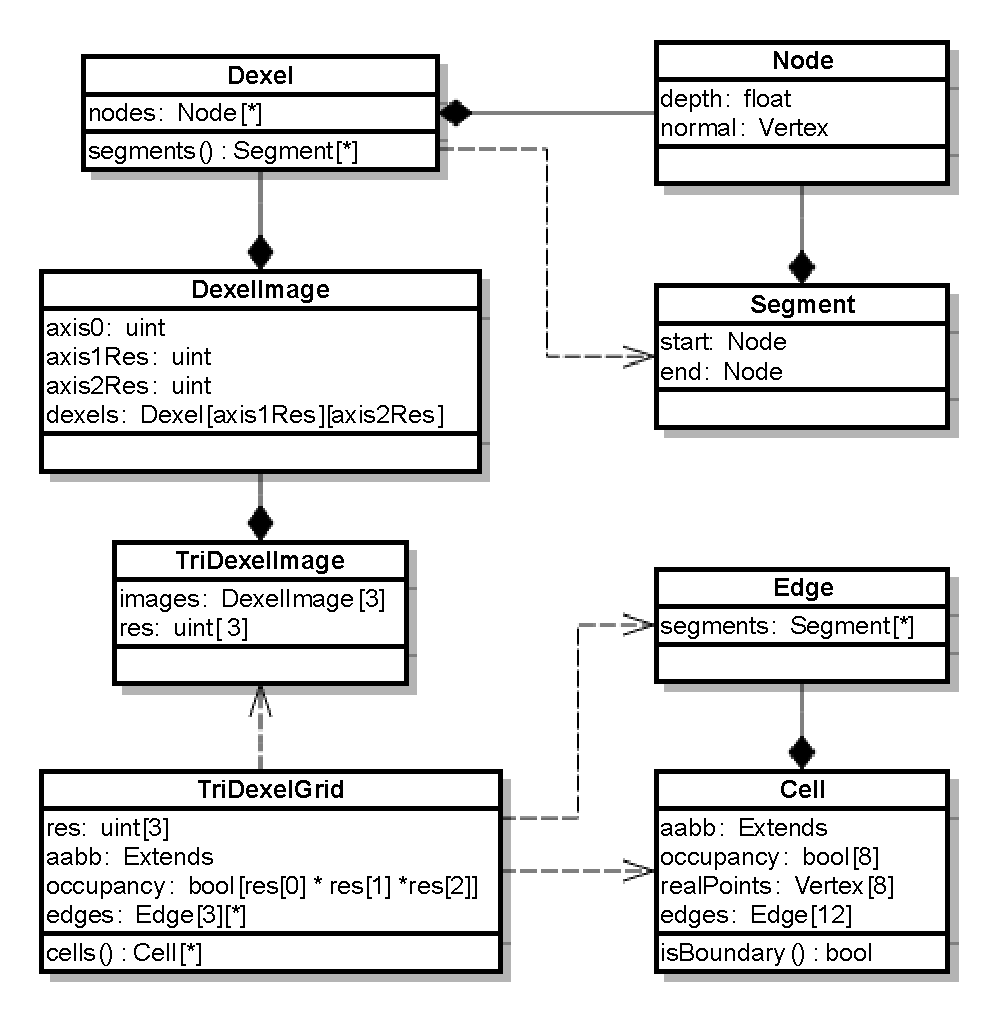
\includegraphics[width=0.9\textwidth]{images/tri_dexel_datamodel}
	\caption{
		Simplified UML class diagram of the types needed for the tri-dexel reconstruction algorithm in addition to the types used by the VML, \cf figure \ref{fig:vml_datamodel}.
	}
	\label{fig:tri_dexel_datamodel}
\end{figure}
%
The most central data structure is the \var{TriDexelGrid} class.
It represents a tri-dexel representation of the complete VML workpiece, prepared for subsequent regularization and triangulation.
In addition to the tri-dexel grid's resolution \var{res} and bounding box \var{aabb}, the \var{TriDexelGrid} class further contains the occupancy information for each grid point in \var{occupancy}, \ie whether a grid point is spanned by a dexel or not, as well as the actual dexel segments between the grid points, stored in \var{edges}.
The \var{cells} method separates all this information into distinct and independent cells.

Each cell is an instance of the \var{Cell} class and contains the same information as the tri-dexel grid, but locally for a single cell.
A cell stores its bounding box \var{box}, the point occupancy of each of the cell's corners in \var{occupancy}, the corners' coordinates in \var{realPoints} and the 12 edges of the cell, stored in \var{edges}.
Each edge of the cell is an instance of \var{Edge} and contains all spanning dexel segments, clamped to the interval between the edge's incident grid points.
Furthermore, a method \var{isBoundary} is provided to check if the cell is a boundary cell, \ie contains occupied and non-occupied grid points, and therefore contains a part of the workpiece's surface.

The \var{TriDexelGrid} is constructed from the \var{TriDexelImage} class, which, fundamentally, contains the same information as the tri-dexel grid.
The difference is substantially clearer from the workflow's point of view.
Whereas the \var{TriDexelGrid} is already prepared for further processing, the \var{TriDexelImage} class only contains the raw data created by raycasting the VML's data model from three orthogonal directions.
This data only consists of the resolution \var{res} used for raycasting as well as three dexel images \var{images} along the three coordinate system axes.

A \var{DexelImage} describes the result of a single raycast along the axis specified in \var{axis0}, where 0 denotes the x-, 1 the y- and 2 the z-axis.
The members \var{axis1Res} and \var{axis2Res} store the resolution of the dexel image along the two cyclically following axes after \var{axis0}.
For example, if \var{axis0} is 1, the y-axis, then \var{axis1Res} and \var{axis2Res} hold the resolutions along the axes 2 and 0, the z- and x-axis.
Finally, \var{dexels} contains all the dexels of the image.

Each \var{Dexel} instance is then essentially a list of nodes, stored in \var{nodes}.
The number of stored nodes after raycasting is always a multiple of two.
As dexel nodes are typically processed in pairs, as dexel segments, a convenience method \var{segments} is provided, which groups adjacent nodes into instances of \var{DexelSegment}.

A \var{DexelSegment} contains these two nodes as \var{start} and \var{end} node.

Finally, the \var{Node} class holds the depth of the node along its dexel, \ie the distance of the node from the plane where the dexels originate, \cf figure \ref{fig:dexel_image}, as well as the normal vector of this surface entry/exit.

Unrelated to the tri-dexel types are two additional classes, which are used in some algorithms during the reconstruction.

The \var{Ray} class represents a ray starting at the vertex \var{origin} and traveling into the direction stored by \var{direction}.

The \var{EdgeVertex} class holds data to represent a vertex on an edge of a tri-dexel cell.
It contains grid point indices for the two points incident to this vertex's edge, a position and the surface normal of the vertex.

Based on the discussed tri-dexel types, the basic reconstruction algorithm is shown in algorithm \ref{alg:tri_dexel}.
%
\begin{algorithm}
	\centering
	\begin{algorithmic}[1]
		\Function{TriDexel}{$\var{grid}, \var{resolution}$}
			\State $\var{box} = \var{Extends}(\var{grid}.\var{aabb}.\var{lower} - \epsilon_{\var{box}}, \var{grid}.\var{aabb}.\var{upper} + \epsilon_{\var{box}})$
			\State $\var{res} = \Call{UniformResolution}{\var{box}, \var{resolution}}$
			\State $\Call{Reconstruct}{\var{grid}, \var{box}, \var{resolution}}$
		\EndFunction
		\\
		\Function{Reconstruct}{$\var{grid}, \var{box}, \var{resolution}$}
			\State $\var{img} = \var{TriDexelImage}(\var{res})$ \label{alg:line:tri_dexel_begin}
			\State $\Call{AxisParallelRaycast}{\var{grid}, \var{box}, \var{res},\hfill\break
				\hspace*{\dimexpr\algorithmicindent*2}(\var{axis}, \var{x}, \var{y}, \var{v}, \var{n}) \rightarrow \var{img}.\var{images}_{\var{axis}}.\var{dexels}_{\var{x}, \var{y}}.\var{nodes}.\var{add}(\var{Node}(\var{v}_{\var{axis}}, \var{n}))}$
			\State $\var{dgrid} = \Call{CreateTriDexelGrid}{\var{img}, \var{box}}$
			\State $\var{triangles} \gets \varnothing$
			\ForAll{$\var{cell} \in \var{dgrid}.\var{cells}()$}
				\State $\Call{RegularizeCell}{\var{cell}}$
				\State $\var{triangles} \gets \var{triangles} \cup \Call{TriangulateCell}{\var{cell}}$
			\EndFor
			\State \Return $\var{triangles}$
		\EndFunction
	\end{algorithmic}
	\caption{
		Abstract workflow of the surface reconstruction using a tri-dexel approach.
	}
	\label{alg:tri_dexel}
\end{algorithm}
%
At the beginning, a slightly enlarged bounding box is calculated for the size of the tri-dexel grid and raycast.
In this way, edge cases with a surface exactly at the grid's border are avoided.
The \textproc{UniformResolution} function takes the user-specified resolution and the tri-dexel grid's bounding box and calculates three resolutions, one for each axis.
The longest one is equal to the specified resolution and the other two are calculated in such a way that the resulting cells of the tri-dexel grid are as cubic as possible.
This tri-dexel grid resolution is used to preallocate space for the tri-dexel image, which is then filled in the subsequent raycasting process.
The remaining part of the algorithm closely follows the concept discussed in the previous section \ref{sec:tri_dexel_concept}.
The subsequent sections discuss the functions and procedures of the algorithm in the order they are used.


\subsection{Raycast}
\label{sec:tri_dexel_raycast}

The raycast is the prime algorithm for converting the VML's data model into a tri-dexel representation.
The raycast is performed with parallel, axis-aligned and equidistant rays.
All rays start at the intersection points of a uniform, 2-dimensional grid placed on one side of the data model's slightly enlarged bounding box and end at the opposite side, \cf figure \ref{fig:dexel_image}.
Three of these raycasts along the three axes of the coordinate system result in three dexel images.
As the raycasting code is kept separated from the tri-dexel data structures, a function is passed to the raycasting code which is invoked each time a ray has found a surface intersection.
Therefore, the same code is capable of creating other data structures as well, \cf chapter \ref{ch:point_cloud_based}.

The entry routine and ray creation code of the raycasting algorithm is shown in algorithm \ref{alg:tri_dexel_raycast}.
%
\begin{algorithm}
	\centering
	\begin{algorithmic}[1]
		\Procedure{Raycast}{$\var{grid}, \var{box}, \var{res}, \var{hitFunc}$}
			\For{$\var{axis0} \gets 0 \To 2$}
				\State $\var{axis1} \gets (\var{axis0} + 1) \bmod 3$
				\State $\var{axis2} \gets (\var{axis0} + 2) \bmod 3$
				\State $\var{xCount} \gets \var{res}_{\var{axis1}}$
				\State $\var{yCount} \gets \var{res}_{\var{axis2}}$
				\State $\Delta \var{x} \gets (\var{box}.\var{upper}_{\var{axis1}} - \var{box}.\var{lower}_{\var{axis1}}) \div (\var{xCount} - 1)$
				\State $\Delta \var{y} \gets (\var{box}.\var{upper}_{\var{axis2}} - \var{box}.\var{lower}_{\var{axis2}}) \div (\var{yCount} - 1)$
				\For{$\var{y} \gets 0 \To \var{yCount} - 1$}
					\For{$\var{x} \gets 0 \To \var{xCount} - 1$}
						\State $\var{ray} = \Call{CreateRay}{\var{box}, \var{axis0}, \var{axis1}, \var{axis2}, \var{\Delta x}, \var{\Delta y}, \var{x}, \var{y}}$
						\State $\Call{CastRay}{\var{grid}, \var{axis0}, \var{axis1}, \var{axis2}, \var{ray},\hfill\break
							\hspace*{\dimexpr\algorithmicindent*5}(\var{v}, \var{n}) \rightarrow \var{hitFunc}(\var{axis0}, \var{x}, \var{y}, \var{v}, \var{n})}$
					\EndFor
				\EndFor
			\EndFor
		\EndProcedure
		\\
		\Function{CreateRay}{$\var{box}, \var{axis0}, \var{axis1}, \var{axis2}, \var{\Delta x}, \var{\Delta y}, \var{x}, \var{y}, \var{xCount}, \var{yCount}$}
			\State $\var{origin} \gets \var{box}.\var{lower}$
			\State $\var{origin}_{\var{axis1}} \gets \var{origin}_{\var{axis1}} + \var{x} \cdot \var{\Delta x}$
			\State $\var{origin}_{\var{axis2}} \gets \var{origin}_{\var{axis2}} + \var{y} \cdot \var{\Delta y}$
			\State $\var{direction} = \var{Vertex}(0, 0, 0)$
			\State $\var{direction}_{\var{axis0}} \gets 1$
			\State \Return $\var{Ray}(\var{origin}, \var{direction})$
		\EndFunction
		\\
		\Procedure{CastRay}{$\var{grid}, \var{axis0}, \var{axis1}, \var{axis2}, \var{ray}, \var{hitFunc}$}
			\State $\var{traverser} \gets \var{AxisAlignedTraverser}(\var{grid}, \var{ray}, \var{axis0}, \var{axis1}, \var{axis2})$
			\While{$\neg \var{traverser}.\var{reachedEnd}()$}
				\State $\var{cell} \gets \var{traverser}.\var{nextCell}()$
				\State $\Call{IntersectCell}{\var{cell}, \var{ray}, \var{axis0}, \var{axis1}, \var{axis2}, \var{hitFunc}}$
			\EndWhile
		\EndProcedure
	\end{algorithmic}
	\caption{
		Basic algorithm for performing a parallel raycast along all three coordinate system axes on the VML's data model.
	}
	\label{alg:tri_dexel_raycast}
\end{algorithm}
%
The outmost procedure \textproc{Raycast} takes four arguments: the VML's regular grid data structure, the bounding box of the raycasted area, the resolution of the raycasted \enquote{image} as well as a function, which is called on every surface hit.
The algorithm starts off by iterating over the three coordinate system's axes.
The index of each axis is stored in the variable \var{axis0}, where 0 denotes the x-, 1 the y- and 2 the z-axis.
\var{axis0} is also called primary axis and is accompanied by \var{axis1} and \var{axis2} which hold the other two, secondary axes, in cyclic order.
Depending on the choice of primary and secondary axes, the resolution of the 2-dimensional grid spawning the rays is determined and assigned to \var{xCount} and \var{yCount}, for the horizontal and vertical resolution.
The coordinate x and y inside the raycasting code refer to the axes of the raycasted \enquote{image} and not the axes of the 3-dimensional coordinate system of the scene.
Afterwards, the distance between two incident rays along both secondary axes is computed.
Therefore, the size of the bounding box is computed and divided by the resolution minus one.
The result is assigned to the variables \var{\Delta x} and \var{\Delta y}.
Now, the algorithm starts creating and casting all rays along their primary axis.
Two nested loops iterate over all points of the 2-dimensional grid spawning rays.
For each grid point at $\var{x}, \var{y}$ a ray is created using the \textproc{CreateRay} function.
Subsequently, the ray is cast into the VML's regular grid by invoking \textproc{CastRay}, passing a closure which is invoked each time a hit is recorded.

The \textproc{CreateRay} function's objective is to create an instance of \var{Ray}, storing the ray's origin and direction.
The origin is calculated by starting from the bounding box's \var{lower} corner.
Along the primary axis, this value is already correct.
On the secondary axes, the origin, currently at the origin for ray $0, 0$, must be moved according to the ray's \var{x} and \var{y} coordinate.
In order to do so, \var{x} and \var{y} are multiplied by the distances between incident rays, \var{\Delta x} and \var{\Delta y}, and added to the origin's secondary axes.
%
Computing the ray's direction is simpler, as it is axis aligned.
Therefore, the direction is a unit vector along the primary axis, created by setting the corresponding component of a zeroed vector to one.
%
Finally, \var{origin} and \var{direction} are aggregated into an instance of \var{Ray} and returned.

After rays have been created, they are cast into the VML's regular grid data structure using the \textproc{CastRay} procedure.
Traversing a ray through a regular grid is done using the 3D-DDA algorithm \cite{3DDDA}, \cf figure \ref{fig:traverser}.
However, as the rays are axis-parallel, traversal essentially boils down to mapping the ray's origin to the appropriate grid cell and incrementing the 3-dimensional cell index along the primary axis until the other end of the grid is reached.
This logic is hidden behind the \var{AxisAlignedTraverser} class and is no further elaborated.

During traversal, the ray is intersected with each cell pulled from the traverser using the \textproc{IntersectCell} algorithm.
Fundamentally, the implementation is based on the inside counting scheme of the visualization code explained in figure \ref{fig:raycast}.
The important difference is that the raycast for visualization may terminate after the first intersection found.
Furthermore, minor inconsistencies are tolerable and may result in a few pixel errors on the final image.
However, when creating dexels, a consistent number of surface entries and exits as well as numerically correct ordering of the intersections is substantial.
Consequently, such an intersection routine must employ a great deal of numeric precautions and extra checks to deliver a correct result, even sacrificing intersections for the sake of consistency.
This procedure forms the heart of the raycasting algorithm.
As it is quite comprehensive and highly tailored to the VML's internal data structures, the detailed pseudocode of the \textproc{IntersectCell} routine is omitted.


\subsection{Tri-dexel image and grid generation}
\label{sec:tri_dexel_dexel_image_generation}

Based on the generic, axis-parallel raycasting routine, a tri-dexel image is created in the base algorithm \ref{alg:tri_dexel}.
Before the raycast is launched, an instance of \var{TriDexelImage} is created, preallocating enough space to hold 3 dexel images, each holding a 2-dimensional grid of empty dexels.
When calling \textproc{AxisParallelRaycast}, an anonymous function is passed, which is invoked on every surface hit detected during raycasting.
This function receives the primary axis \var{axis}, \ie the axis along which the rays where traversed, \var{x} and \var{y} coordinate on the 2-dimensional dexel grid as well as the intersection point \var{v} with the normal of the hit triangle \var{n}.
With this information, the tri-dexel image stored in \var{img} is populated.
Once raycasting has completed, the tri-dexel grid is generated from the tri-dexel image.
This conversion is more a reinterpretation and preparation of the information contained within the tri-dexel image.
Whereas the image contains the raw raycasting result, the tri-dexel grid already stores grid point occupancy information and cuts all dexels at cell borders.
This preparation eases the follow-up processing of individual cells.

Converting the tri-dexel image into a tri-dexel grid is done by the \textproc{CreateTriDexelGrid} function, which is shown in algorithm \ref{alg:tri_dexel_grid_generation}.
%
\begin{algorithm}
	\centering
	\begin{algorithmic}[1]
		\Function{CreateTriDexelGrid}{$\var{triImage}, \var{box}$}
			\State $\var{res} = \var{triImage}.\var{res}$
			\State $\var{grid} = \var{TriDexelGrid}(\var{res}, \var{box})$ \Comment{$\forall \var{x}, \var{y}, \var{z} \colon \var{grid}.\var{occupancy}_{\var{x}, \var{y}, \var{z}} = \False$}
			\For{$\var{axis0} \gets 0 \To 2$}
				\State $\var{axis1} \gets (\var{axis0} + 1) \bmod 3$
				\State $\var{axis2} \gets (\var{axis0} + 2) \bmod 3$
				\State $\var{image} \gets \var{triImage}.\var{images}_{\var{axis0}}$
				\For{$\var{axis1Val} \gets 0 \To \var{res}_{\var{axis1}} - 1$}
					\For{$\var{axis2Val} \gets 0 \To \var{res}_{\var{axis2}} - 1$}
						\State $\var{dexel} \gets \var{image}.\var{dexels}_{\var{axis1Val}, \var{axis2Val}}$
						\ForAll{$\var{seg} \in \var{dexel}.\var{segments}()$}
							\LineComment{Compute affected grid point range}
							\State $\var{start} \gets \Call{DepthToGrid}{\var{seg}.\var{start}.\var{depth}, \var{axis0}, \var{res}, \var{box}}$
							\State $\var{end} \gets \Call{DepthToGrid}{\var{seg}.\var{end}.\var{depth}, \var{axis0}, \var{res}, \var{box}}$
							\For{$\var{axis0Val} \gets \var{start} \To \var{end}$}
								%\State $\var{gridFrom} \gets (0, 0, 0)$
								\State $\var{gridFrom}_{\var{axis0}} \gets \var{axis0Val}$
								\State $\var{gridFrom}_{\var{axis1}} \gets \var{axis1Val}$
								\State $\var{gridFrom}_{\var{axis2}} \gets \var{axis2Val}$
								\State $\var{gridTo} \gets \var{gridFrom}$
								\State $\var{gridTo}_{\var{axis0}} \gets \var{gridTo}_{\var{axis0}} + 1$
								\State $\var{depthFrom} = \Call{GridToDepth}{\var{gridFrom}_{\var{axis0}}, \var{axis0}, \var{res}, \var{box}}$
								\State $\var{depthTo}   = \Call{GridToDepth}{\var{gridTo}_{\var{axis0}}, \var{axis0}, \var{res}, \var{box}}$
								\LineComment{Point occupancy}
								\If{$\var{seg}.\var{start}.\var{depth} \leq \var{depthFrom} \leq \var{seg}.\var{end}.\var{depth}$}
									\State $\var{grid}.\var{occupancy}_{\var{gridFrom}} \gets \True$
								\EndIf
								\If{$\var{seg}.\var{start}.\var{depth} \leq \var{depthTo} \leq \var{seg}.\var{end}.\var{depth}$}
									\State $\var{grid}.\var{occupancy}_{\var{gridTo}} \gets \True$
								\EndIf
								\LineComment{Copy segment and clamp to cell border}
								\State $\var{s} \gets \var{seg}$
								\If{$\var{s}.\var{start}.\var{depth} < \var{depthFrom}$}
									\State $\var{s}.\var{start}.\var{depth} \gets \var{depthFrom}$
								\EndIf
								\If{$\var{s}.\var{end}.\var{depth} > \var{depthTo}$}
									\State $\var{s}.\var{end}.\var{depth} \gets \var{depthTo}$
								\EndIf
								\State $\var{grid}.\var{edges}_{\var{axis0}, \var{gridFrom}}.\var{segments}.\var{add}(\var{s})$ \label{alg:line:grid_edge_insertion}
							\EndFor
						\EndFor
					\EndFor
				\EndFor
			\EndFor
		\EndFunction
		\\
		\Function{DepthToGrid}{\var{depth}, \var{axis}, \var{res}, \var{box}}
			\State \Return $\floor{(\var{depth} - \var{box}.\var{lower}_{\var{axis}}) \div (\var{box}.\var{upper}_{\var{axis}} - \var{box}.\var{lower}_{\var{axis}}) \cdot (\var{res}_{\var{axis}} - 1)}$
		\EndFunction
		\\
		\Function{GridToDepth}{\var{gridCoord}, \var{axis}, \var{res}, \var{box}}
			\State \Return $\var{gridCoord} \div (\var{res}_{\var{axis}} - 1) \cdot (\var{box}.\var{upper}_{\var{axis}} - \var{box}.\var{lower}_{\var{axis}}) + \var{box}.\var{lower}_{\var{axis}}$
		\EndFunction
	\end{algorithmic}
	\caption{
		Creating a tri-dexel grid from the raycasted dexel images.
	}
	\label{alg:tri_dexel_grid_generation}
\end{algorithm}
%
The algorithm starts by constructing an instance of the \var{TriDexelGrid} class.
During this construction, \ie the constructor, the occupancy of each grid point is set to \False.
Furthermore, space to hold all edges of the tri-dexel grid is allocated.
Accessing grid edges, \ie subscripting the member \var{edges}, is done by supplying the axis to which the edge is parallel as well as a three dimensional position.
Afterwards, the algorithm iterates over all three axes of the coordinate system and therefore over the three dexel images of the tri-dexel image.
For each dexel image further loops are necessary to iterate over all dexels of the image and for each dexel over its segments.

For each segment the affected range of grid points is computed.
Two coordinates of these points are already known, which are the same as the coordinates of the dexel in its image.
The third, missing coordinates are the ones spanned by the dexel segment.
To compute these coordinates, the dexel segment's start and end depth are mapped to grid point coordinates.
Each call to \textproc{DepthToGrid} yields the lower grid point coordinate along the specified axis for a given depth on this axis.
This value is also equivalent to the index of the edge along \var{axis} on which a dexel node with the given depth would lie.
The computed range, \var{start} to \var{end}, in conjunction with \var{axis1Val} and \var{axis2Val}, now gives all indices of the affected grid points and edges.

The innermost loop finally iterates over all edges of the tri-dexel grid spanned by the current dexel segment \var{seg}.
The variables \var{gridFrom} and \var{gridTo} are the indices of the grid points incident to the current edge, which's index is also \var{gridFrom}.
For both grid points of the current edge a depth value along the current axis is calculated.
Two conditionals then compare these depth values against the start and end depth of the current dexel segment.
If the depth of any grid point is between a dexel segment's start and end depth, \ie the segment spans the grid point, it is marked as occupied by setting the corresponding element of the grid's \var{occupancy} member.
After this point occupancy check, the segment must also be added to the current edge, incident to the grid points \var{gridFrom} and \var{gridTo}.
As the cells of the tri-dexel grid are later processed independently and to make some calculations easier, the dexel-segments are further clamped to the cell's bounds, \ie constrained to the range of the cell's grid point's depth values.
Therefore, a copy of the current segment is made and the start and end depth set to the respective grid point's depth values, in case they are outside.
Finally, the clamped segment is added to the current edge.

After \textproc{CreateTriDexelGrid} returned, the tri-dexel image is no longer needed, as the semantically equivalent information is stored in the newly created tri-dexel grid.
The main algorithm, algorithm \ref{alg:tri_dexel}, may release resources held for the \var{img} variable now.

The newly created tri-dexel grid \var{dgrid} is now used to iterate over all cells and process them further.
The call to $\var{dgrid}.\var{cells}()$, for each cell, collects all data from the tri-dexel grid belonging to a single cell into an instance of \var{Cell}.
The created cells contain deep copies of the grid's data, as the cell's edges are shared with neighboring cells, but will be modified in subsequent parts of the algorithm.
This poses no problem in a single threaded context, but would lead to data races when multiple cells are processed concurrently, \cf section \ref{sec:tri_dexel_parallelization}.


\subsection{Regularization}
\label{sec:tri_dexel_regularization}

During the conversion of the VML's data model into a tri-dexel representation errors may occur.
Dexel segments for example might not be of accurate length because of numerics in the triangle intersection routine or corrections applied by the raycaster when sorting and counting through the intersected structures to identify surface hits.
Such defects are especially critical at the intersection points of dexels from multiple dexel images, the grid points.
Furthermore, the number of different configurations a single tri-dexel cell may have is huge, as each edge may contain an arbitrary number of dexel segments, rendering the creation of an appropriate triangulation algorithm almost impossible.
It is thus beneficial to reduce the number of cases by dropping some information in favor of regularity.

The process of repairing defects and reducing complexity of a tri-dexel cell is called regularization.
This method is documented well in the tri-dexel paper foundational to this chapter \cite{tridexel_reconstruction}.
Regularizing a tri-dexel cell is done by iterating over all edges and applying a set of rules.
These rules are illustrated in figure \ref{fig:tri_dexel_regularization} and are as follows:

\begin{figure}[h]
	%\renewcommand{\thesubfigure}{\arabic{subfigure}}
	\centering
	\begin{subfigure}[t]{0.45\textwidth}
		\centering
		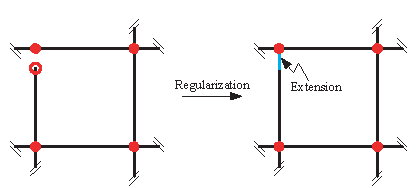
\includegraphics[width=\textwidth]{images/tri_dexel_regularization_1}
		\caption{Two occupied points.}
		\label{fig:tri_dexel_regularization_1}
	\end{subfigure}
	\begin{subfigure}[t]{0.45\textwidth}
		\centering
		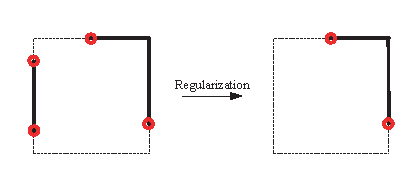
\includegraphics[width=\textwidth]{images/tri_dexel_regularization_2}
		\caption{Two non-occuupied points}
		\label{fig:tri_dexel_regularization_2}
	\end{subfigure}
	\begin{subfigure}[t]{0.45\textwidth}
		\centering
		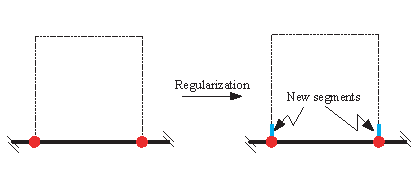
\includegraphics[width=\textwidth]{images/tri_dexel_regularization_3}
		\caption{One occupied point with no segment}
		\label{fig:tri_dexel_regularization_3}
	\end{subfigure}
	\begin{subfigure}[t]{0.45\textwidth}
		\centering
		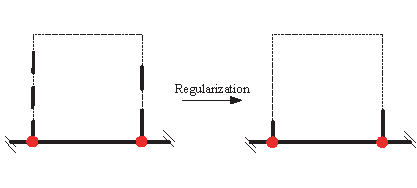
\includegraphics[width=\textwidth]{images/tri_dexel_regularization_4}
		\caption{Deletion of non-spanning segments}
		\label{fig:tri_dexel_regularization_4}
	\end{subfigure}
	\caption{
		The four regularization rules which are applied to each tri-dexel cell before it is triangulated.
		Image adapted from \cite{tridexel_reconstruction}.
	}
	\label{fig:tri_dexel_regularization}
\end{figure}

\begin{enumerate}
	\item If two adjacent grid points are marked as occupied, the incident edge must contain exactly one dexel segment with start and end depth exactly at the corresponding depths of the grid points.
	Figure \ref{fig:tri_dexel_regularization_1} shows the extension of the leftmost segment to touch the occupied grid point in the upper left.

	\item If two adjacent grid points are not marked as occupied, the incident edge must not contain any dexel segments.
	Figure \ref{fig:tri_dexel_regularization_2} shows the removal of the leftmost segment from an edge between two non-occupied grid points.

	\item If an edge, which is incident to only one occupied grid point, does not contain a dexel segment touching this point, a short segment is added, or, if a segment exists and is close enough to the occupied grid point, it is extended to touch the occupied point.
	Figure \ref{fig:tri_dexel_regularization_3} shows the creation of two small dexel segments at both lower grid points as the left and right edge do not contain any segments.

	\item If any segment does not touch any of the two incident grid points, it is removed.
	Figure \ref{fig:tri_dexel_regularization_4} shows the removal of segments on the left and right edge which do not touch any grid point.
\end{enumerate}

%These rules are applied to each cell of the tri-dexel grid constructed so far.
The implementation of these regularization rules, \ie the \textproc{RegularizeCell} routine, is detailed in algorithm \ref{alg:tri_dexel_regularization}.
%
\begin{algorithm}
	\centering
	\begin{algorithmic}[1]
		\Function{RegularizeCell}{$\var{cell}$}
			\For{$ \var{i} \gets 0 \To 11 $}
				\State $\var{segs} \gets \var{cell}.\var{edge}_{\var{i}}.\var{segments}$ \Comment{reference only}
				\label{alg:line:reg_vars_begin}
				\State $(\var{src}, \var{dst}) \gets \var{edgeToPointIds}_{\var{i}}$
				\State $\var{axis} \gets \var{edgeToAxis}_{\var{src}, \var{dst}}$
				\State $\var{srcPoint} \gets \var{cell}.\var{realPoints}_{\var{src}}$
				\State $\var{dstPoint} \gets \var{cell}.\var{realPoints}_{\var{dst}}$
				\State $\var{srcDepth} \gets \var{srcPoint}_{\var{axis}}$
				\State $\var{dstDepth} \gets \var{dstPoint}_{\var{axis}}$
				\State $\var{srcOcc} \gets \var{cell}.\var{occupancy}_{\var{src}}$
				\State $\var{dstOcc} \gets \var{cell}.\var{occupancy}_{\var{dst}}$
				\label{alg:line:reg_vars_end}

				\LineComment{Rule 1}
				\If{$\var{srcOcc} \wedge \var{dstOcc}$}
					\State $\var{n} \gets \var{Vertex}()$ \Comment{Invalid normal}
					\State $\var{segs} = \{ \var{Segment}(\var{Node}(\var{srcDepth}, \var{n}), \var{Node}(\var{dstDepth}, \var{n})) \}$
				\EndIf

				\LineComment{Rule 2}
				\If{$\neg \var{srcOcc} \wedge \neg \var{dstOcc}$}
					\State $\var{segs} \gets \varnothing$
				\EndIf

				\LineComment{Rule 3}
				\State $\var{n} = \var{Vertex}(0, 0, 0)$
				\State $\var{n}_{\var{axis}} = 1$
				\If{$\var{srcOcc} \wedge \neg \var{dstOcc}$}
					\If{$|\var{segs}| = 0 \vee \var{segs}_0.\var{start}.\var{depth} - \rho > \var{srcDepth}$}
						\State $\var{segs}.\var{add}(\var{Segment}(\var{Node}(\var{srcDepth}, -\var{n}), \var{Node}(\var{srcDepth} + \rho, \var{n})))$ % TODO: check if add_front is necessary
					\ElsIf{$|\var{segs}| > 0 \wedge \var{segs}_0.\var{start}.\var{depth} > \var{srcDepth} \wedge {}$\hfill\break
						\hspace*{\dimexpr\algorithmicindent*4}$\var{segs}_0.\var{start}.\var{depth} - \rho \leq \var{srcDepth}$}
						\State $\var{segs}_0.\var{start}.\var{depth} \gets \var{srcDepth}$
					\EndIf
				\EndIf
				\If{$\neg \var{srcOcc} \wedge \var{dstOcc}$}
					\If{$|\var{segs}| = 0 \vee \var{segs}_{|\var{segs}| - 1}.\var{end}.\var{depth} + \rho < \var{dstDepth}$}
						\State $\var{segs}.\var{add}(\var{Segment}(\var{Node}(\var{dstDepth} - \rho, -\var{n}), \var{Node}(\var{dstDepth}, \var{n})))$
					\ElsIf{$|\var{segs}| > 0 \wedge \var{segs}_{|\var{segs}| - 1}.\var{end}.\var{depth} < \var{dstDepth} \wedge {}$\hfill\break
						\hspace*{\dimexpr\algorithmicindent*4}$\var{segs}_{|\var{segs}| - 1}.\var{end}.\var{depth} + \rho \geq \var{dstDepth}$}
						\State $\var{segs}_{|\var{segs}| - 1}.\var{end}.\var{depth} \gets \var{dstDepth}$
					\EndIf
				\EndIf

				\LineComment{Rule 4}
				\ForAll{$\var{s} \in \var{segs}$}
					\If{$\var{s}.\var{start}.\var{depth} \neq \var{srcDepth} \wedge \var{s}.\var{end}.\var{depth} \neq \var{dstDepth}$}
						\State $\var{segs}.\var{remove}(\var{s})$
					\EndIf
				\EndFor
			\EndFor
		\EndFunction
	\end{algorithmic}
	\caption{
		Regularizing a cell of the tri-dexel grid by applying the four rules specified in figure \ref{fig:tri_dexel_regularization}.
	}
	\label{alg:tri_dexel_regularization}
\end{algorithm}
%
Regularizing a cell essentially boils down to processing all 12 edges of the cell, indexed from 0 to 11.
For each edge a bit of meta information is retrieved using some lookup tables.
These tables are shown in figure \ref{fig:tri_dexel_tables} and relate cell corners, edges and axes.
%
\begin{figure}
	\centering
	\begin{subfigure}[t]{0.25\textwidth}
		\centering
		\begin{align*}
			\shortintertext{neighborIds:}
			0 &\colon (1, 4, 2) \\
			1 &\colon (0, 3, 5) \\
			2 &\colon (0, 6, 3) \\
			3 &\colon (1, 2, 7) \\
			4 &\colon (0, 5, 6) \\
			5 &\colon (1, 7, 4) \\
			6 &\colon (2, 4, 7) \\
			7 &\colon (3, 6, 5)
		\end{align*}
	\end{subfigure}%
	\begin{subfigure}[t]{0.25\textwidth}
		\centering
		\begin{align*}
			\shortintertext{edgeToPointIds:}
			 0 &\colon (0, 1) \\
			 1 &\colon (2, 3) \\
			 2 &\colon (4, 5) \\
			 3 &\colon (6, 7) \\
			 4 &\colon (0, 2) \\
			 5 &\colon (1, 3) \\
			 6 &\colon (4, 6) \\
			 7 &\colon (5, 7) \\
			 8 &\colon (0, 4) \\
			 9 &\colon (1, 5) \\
			10 &\colon (2, 6) \\
			11 &\colon (3, 7)
		\end{align*}
	\end{subfigure}%
	\begin{subfigure}[t]{0.25\textwidth}
		\centering
		\begin{align*}
			\shortintertext{pointsToEdgeId:}
			(0, 1), (1, 0) &\colon  0 \\
			(2, 3), (3, 2) &\colon  1 \\
			(4, 5), (5, 4) &\colon  2 \\
			(6, 7), (7, 6) &\colon  3 \\
			(0, 2), (2, 0) &\colon  4 \\
			(1, 3), (3, 1) &\colon  5 \\
			(4, 6), (6, 4) &\colon  6 \\
			(5, 7), (7, 5) &\colon  7 \\
			(0, 4), (4, 0) &\colon  8 \\
			(1, 5), (5, 1) &\colon  9 \\
			(2, 6), (6, 2) &\colon 10 \\
			(3, 7), (7, 3) &\colon 11
		\end{align*}
	\end{subfigure}%
	\begin{subfigure}[t]{0.25\textwidth}
		\centering
		\begin{align*}
			\shortintertext{edgeToAxis:}
			(0, 1), (1, 0) &\colon 0 \\
			(2, 3), (3, 2) &\colon 0 \\
			(4, 5), (5, 4) &\colon 0 \\
			(6, 7), (7, 6) &\colon 0 \\
			(0, 2), (2, 0) &\colon 1 \\
			(1, 3), (3, 1) &\colon 1 \\
			(4, 6), (6, 4) &\colon 1 \\
			(5, 7), (7, 5) &\colon 1 \\
			(0, 4), (4, 0) &\colon 2 \\
			(1, 5), (5, 1) &\colon 2 \\
			(2, 6), (6, 2) &\colon 2 \\
			(3, 7), (7, 3) &\colon 2
		\end{align*}
	\end{subfigure}
	\begin{subfigure}[t]{0.4\textwidth}
		\centering
		\begin{align*}
			\shortintertext{cellSideNormals:}
			\binom{\{0, 2, 4, 6\}}{3} &\colon (         - 1,\phantom{-}0,\phantom{-}0) \\
			\binom{\{1, 3, 5, 7\}}{3} &\colon (\phantom{-}1,\phantom{-}0,\phantom{-}0) \\
			\binom{\{0, 1, 4, 5\}}{3} &\colon (\phantom{-}0,         - 1,\phantom{-}0) \\
			\binom{\{2, 3, 6, 7\}}{3} &\colon (\phantom{-}0,\phantom{-}1,\phantom{-}0) \\
			\binom{\{4, 5, 6, 7\}}{3} &\colon (\phantom{-}0,\phantom{-}0,         - 1) \\
			\binom{\{0, 1, 2, 3\}}{3} &\colon (\phantom{-}0,\phantom{-}0,\phantom{-}1) \\
		\end{align*}
	\end{subfigure}
	\caption{
		Helper tables used by regularization and triangulation algorithms.
	}
	\label{fig:tri_dexel_tables}
\end{figure}
%
For a given edge index, the indices of the incident grid points are retrieved, called \var{src} and \var{dst}, where \var{src} is always the grid point with the lower depth value.
In addition to the index, the coordinate and occupancy is also retrieved in \var{srcPoint}, \var{dstPoint}, \var{srcOcc} and \var{dstOcc}.
Finally, the axis parallel to the edge is looked up and stored in \var{axis}.
Afterwards, the algorithm starts to apply the regularization rules.

For the first rule, the occupancy of both grid points is checked.
If both of them are occupied, the existing segments on the edge are replaced by a new set with a new segment spanning from the source to the destination grid point.
As both incident grid points are occupied, the edge cannot contain a surface intersection.
Therefore, the normals on the dexel nodes can be safely ignored.

The second rule states that if both grid points are not occupied, the incident edge must be empty.
Thus, in this case, all segments are simply replaced by an empty set.

Rule three is applied if only one grid point is marked as occupied.
If segments are present on the current edge, the algorithm tests whether the first or last segment touches the occupied grid point, or is very close to it.
If the source point is marked, the first segment's start must touch or be near to it, \ie the start node's depth must not be further away from the grid point than a small $\rho$.
This length may be chosen arbitrarily, but as its purpose is to correct a numeric issue, a tiny value is sufficient.
In case the destination point is marked, the last segment's end must touch or be near it.
If existing segments are nearer than $\rho$ to an occupied grid point, they are extended to reach it.
If there are no segments on the edge or the present segments are not in close proximity to their appropriate points, a new dexel segment is added.
The new segment starts at the occupied grid point and has a small length of $\rho$.
Regarding the normal, the surface intersection represented by the newly added segment might be used by a later triangulation.
However, the true normal is stored on the numerically too short segment in the appropriate neighboring cell, which is hard to retrieve as the tri-dexel grid's cells are isolated to allow independent processing.
Hence, an artificial normal is added in the direction of the edge's axis.

The last rule, rule 4, finally checks all segments if they touch at least one grid point.
If any segment does not satisfy this condition, the segment is removed.

After all 4 rules have been applied to all 12 edges of the cell, the cell is regularized and fulfills a few properties:
\begin{itemize}
	\item Between two occupied grid points, there is always one full segment.
	\item Between two non-occupied grid points, there is never a segment.
	\item Between two differently marked grid points, there is exactly one segment with one node's depth not equal to the depth of any grid point.
\end{itemize}
These properties now allow for a subsequent triangulation.


\subsection{Triangulation}
\label{sec:tri_dexel_triangulation}

After regularization, a cell of the tri-dexel grid is ready for triangulation.
The process of creating triangles from a cell is done in three steps where the second one is optional.
Firstly, set of boundary loops is created from the grid points and dexel nodes between them.
Secondly, from the loop, vertex and normal information, optional feature points are created.
Thirdly, the boundary loops with optional feature information are triangulated.

For the initial boundary loop discovery, a depth-first search process is iteratively started at non-occupied grid points of the cell.
The search traverses the cell's edges and backtracks each time an occupied grid point and therefore a grid edge containing a dexel node is found.
Traversed grid points are marked as visited and cause future searches to backtrack immediately.
The list of visited grid edges containing dexel nodes, per search, in the order they were visited, form a boundary loop.
A cell might contain multiple boundary loops, which are found in multiple searches when starting at different, non-occupied grid points.

Figure \ref{fig:tri_dexel_triangulation} illustrates this depth-search process by two examples.
%
\begin{figure}
	\centering
	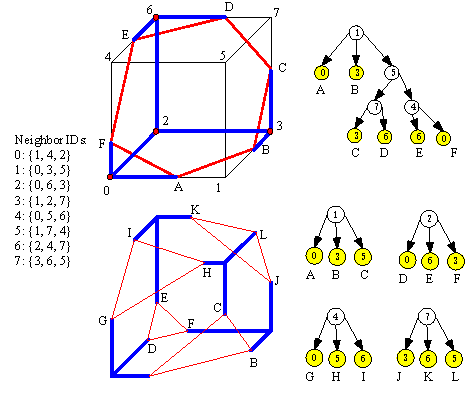
\includegraphics[width=0.9\textwidth]{images/tri_dexel_triangulation}
	\caption{
		Triangulating a tri-dexel cell by finding boundary loops using depth-first search along the cube, starting at non-occupied nodes \cite{tridexel_reconstruction}.
	}
	\label{fig:tri_dexel_triangulation}
\end{figure}
%
In the upper example, a single boundary loop is discovered.
The search starts at grid point 1.
At each grid point, a list of neighbors has to be retrieved.
These neighbor ids make up a small table which is listed in figure \ref{fig:tri_dexel_tables} and beside the two examples in figure \ref{fig:tri_dexel_triangulation}.
The neighbors of a grid point are further traversed in counter-clockwise order, starting at the next neighbor after the one from which the current grid point has been reached.
At the first grid point of the search, the neighbor to start with may be chosen freely, and is usually the first one of the neighbor ids table.
At grid point 1, the neighbors 0, 3 and 5 are traversed.
Neighbors 0 and 3 reach an occupied grid point and therefore cause the search to backtrack, storing the dexel nodes A and B on the edges to 0 and 3.
As the neighbor 5 is non-occupied, the search continues with its neighbors, 1, 7, and 4.
Grid point 1 is omitted, as it has already been visited.
Grid point 7 is further traversed and backtracks at point 3 and 6, resulting in the dexel nodes C and D.
Grid point 4 produces the nodes E and F.
Afterwards, the search backtracks until the starting point is reached and terminates.
In visited order, the dexel nodes A to F form a boundary loop.
Further searches started at other grid points immediately return as all non-occupied nodes have already been visited by the search started at point 1.
%
In the lower example of figure \ref{fig:tri_dexel_triangulation}, the depth-first search discovers multiple boundary loops.

Triangulating a cell with occupancy information at its corners and vertices on its edges into triangles is a problem which is also discussed in voxel-based surface reconstruction techniques, such as the marching cubes variants.
In fact, a tri-dexel cell with 8 Boolean occupancy values at the corners represents one of $2^8 = 256$ cases.
Therefore, the boundary loop configuration and also the triangulation could be precomputed for each case and stored in a lookup table.
This strategy is typically found in the original and many derived marching cubes implementations \cite{marching_cubes}.
As a matter of fact, the tables used by these marching cubes implementations, actually any table, could be used to triangulate tri-dexel cells.

Unfortunately, the depth-first search approach, as explained in the corresponding paper \cite{tridexel_reconstruction}, does have an issue with 4 of the 256 configurations.
If only two grid points are occupied and lie on diagonally opposing corners of the cell, they form two boundary loops which are both discoverable by a single depth-first search.
This causes a problem, as the search discovers 6 vertices, which do not make up a single but two loops.
Therefore, these cases have to be handled differently.
A simple solution is to just start the depth-first search at the occupied grid points, resulting in two loops, and reverse the vertex order.

Algorithm \ref{alg:tri_dexel_triangulation} shows the basic triangulation of a tri-dexel cell without any feature reconstruction.
%
\begin{algorithm}
	\centering
	\begin{algorithmic}[1]
		\Function{TriangulateCell}{$\var{cell}$}
			%\State $loops$
			\If{$\neg \Call{IsProblematicCase}{\var{cell}}$}
				\State $\var{loops} \gets \Call{FindLoops}{\var{cell}, \False}$
			\Else
				\State $\var{loops} \gets \Call{ReverseLoops}{\Call{FindLoops}{\var{cell}, \True}}$
			\EndIf
			\State $\var{triangles} \gets \varnothing$
			\For{$\var{loop} \in \var{loops}$}
				\State $\var{triangles} \gets \var{triangles} \cup \Call{TriangulateLoopSimple}{\var{loop}}$
			\EndFor
			\State \Return $\var{triangles}$
		\EndFunction
		\\
		\Function{FindLoops}{$\var{cell}, \var{occupied}$}
			\State $\var{visited} \gets \var{array}(8, \False)$
			\State $\var{loops} \gets \varnothing$
			\For{$\var{start} \gets 0 \To 7$}
				\State $\var{loop} \gets \var{array}()$
				\State $\Call{DepthFirstSearch}{\var{occupied}, \var{start}, -1, \var{cell}, \var{visited}, \var{loop}}$
				\If{$|\var{loop}| > 0$}
					$\var{loops}.\var{add}(\var{loop})$
				\EndIf
			\EndFor
			\State \Return $\var{loops}$
		\EndFunction
		\\
		\Function{DepthFirstSearch}{$\var{occupied}, \var{cur}, \var{last}, \var{cell}, \var{visited}, \var{loop}$}
			\If{$\var{cell}.\var{occupancy}_{\var{cur}} = \var{occupied} \wedge \neg \var{visited}_{\var{cur}}$}
				\State $\var{visited}_{\var{cur}} \gets \True$
				\State $\var{neighbors} \gets \Call{RotateToStartAfter}{\var{neighborIds}_{\var{cur}}, \var{last}}$
				\For{$\var{n} \in \var{neighbors}$}
					\If{$\var{cell}.\var{occupancy}_{\var{n}} \neq \var{occupied}$}
						\State $\var{axis} \gets \var{edgeToAxis}_{\var{cur}, \var{n}}$
						\State $\var{seg} \gets \var{cell}.\var{edges}_{\var{pointsToEdgeId}_{\var{cur}, \var{n}}}.\var{segments}_0$
						\State $\var{curReal} \gets \var{cell}.\var{realPoints}_{\var{cur}}$
						\State $\var{nReal} \gets \var{cell}.\var{realPoints}_{\var{n}}$
						\If{$\var{seg}.\var{start}.\var{depth} = \var{curReal}_{\var{axis}} \vee \var{seg}.\var{start}.\var{depth} = \var{nReal}_{\var{axis}}$}
							\State $\var{node} \gets \var{seg}.\var{end}$
						\Else
							\State $\var{node} \gets \var{seg}.\var{start}$
						\EndIf
						\State $\var{v} \gets \var{curReal}$
						\State $\var{v}_{\var{axis}} \gets \var{node}.\var{depth}$
						\State $\var{loop}.\var{add}(\var{EdgeVertex}(\var{cur}, \var{n}, \var{v}, \var{node}.\var{normal}))$
					\Else
						\State $\Call{DepthFirstSearch}{\var{occupied}, \var{n}, \var{cur}, \var{cell}, \var{visited}, \var{loop}}$
					\EndIf
				\EndFor
			\EndIf
		\EndFunction
		\\
		\Function{TriangulateLoopSimple}{$\var{loop}$}
			\State $\var{vertices} \gets \Call{Map}{\var{loop}, \var{v} \rightarrow \var{v}.\var{position}}$
			\State \Return $\Call{TriangulateLoopIntoFan}{\var{vertices}}$
		\EndFunction
	\end{algorithmic}
	\caption{
		Basic triangulating routine for a tri-dexel cell.
		No refinement or feature reconstruction is done.
	}
	\label{alg:tri_dexel_triangulation}
\end{algorithm}
%
The \textproc{TriangulateCell} function begins by checking if the cell is one of the 4 problematic cases, \ie cases with two, diagonally opposing occupied grid points.
In non-problematic cases, the \textproc{FindLoops} function is called, starting at non-occupied vertices.
In problematic cases, the loop search routine is started at occupied vertices and the resulting loops are reversed.

After all loops have been identified, they are sent to the \textproc{TriangulateLoopSimple} function which generates triangles from the loop.
The union of all triangulated loops is returned as triangulation result of the given tri-dexel cell.

The \textproc{FindLoops} algorithm is the entry into the depth-first search based traversal of the cell's edges as shown in figure \ref{fig:tri_dexel_triangulation}.
It starts by initializing an array with 8 Boolean values, set to false.
These values keep track of the already visited vertices.
For each of the 8 possible start grid points an empty array \var{loop} is created, which is passed recursively through the following depth-first search.
It collects information about the encountered dexel nodes, in the order they are visited, to form a boundary loop.
The call to \textproc{DepthFirstSearch} then starts traversing the cell's edges starting at the grid point \var{start}.
After the call has returned, a conditional checks if loop vertices have been found and adds the loop in this case.
After a search has been launched from each start point, the set of collected loops is returned.

The recursive \textproc{DepthFirstSearch} algorithm is the heart of the boundary loop discovery.
Initially, it checks if the current grid point is equal to \var{occupied} and has not been visited yet.
The parameter \var{occupied} is usually false for the default case, \ie the search traverses on non-occupied points, and only true in problematic cases.
If both conditions are met, the point is marked as visited and the list of neighbor points is fetched.
This list is rotated to start at the index right after the one the search came from.
This rotation ensures, that each neighbor is visited in counter-clockwise order as seen from the incoming edge.
In case of the first call to \textproc{DepthFirstSearch}, there is no last visited point, \var{last} is $-1$, and the neighbor list is not rotated.
On each neighboring grid point, its occupancy is checked for inequality to \var{occupied}.
If this is true, then \var{cur} and \var{n} have different occupancy and the edge between them contains a vertex of the surface.
This vertex is now constructed from the corresponding dexel node together with some meta data.
Using the \var{edgeToAxis} table of figure \ref{fig:tri_dexel_tables}, the axis parallel to the current edge is obtained.
Using \var{pointsToEdgeId}, the segment on the corresponding cell's edge is also retrieved.
Furthermore, the coordinates of the current and neighboring grid point are stored in local variables.
The \var{node} variable is then set to the dexel node which does not touch one of the grid points.
The vertex on the current edge is then constructed starting with the coordinate of the current grid point \var{curReal}.
Choosing the neighboring grid point's coordinate is also valid, as both coordinates only differ at the component at \var{axis}.
This component of the new vertex is then set to the selected node's depth.
Finally, an instance of \var{EdgeVertex} is added to the boundary loop, containing both grid point's ids, the newly calculated vertex and the corresponding surface normal as obtained from the dexel node.
Afterwards, the function returns and the search backtracks.
In case the current neighbor's occupancy is equal to \var{occupied}, \ie no vertex on the current edge, the depth-first search is recursively continued with the current point index passed as last and the neighbor index passed as current.

Finally, in algorithm \ref{alg:tri_dexel_triangulation}, the \textproc{TriangulateLoopSimple} function just maps each \var{EdgeVertex} of the passed loop to its position, creating a pure list of 3-dimensional vertices.
These vertices are then sent to the \textproc{TriangulateLoopIntoFan} function, which creates a triangle fan from the given vertices around their center of mass.

The \textproc{TriangulateLoopIntoFan} function is one of three loop triangulation primitives used throughout this chapter.
These primitives are listed in algorithm \ref{alg:tri_dexel_loop_triangulation_primitives}.
%
\begin{algorithm}
	\centering
	\begin{algorithmic}[1]
		\Function{TriangulateLoopIntoFan}{$\var{loop}, \var{center}$}
			\If{$|\var{loop}| < 3$}
				\State \Return $\varnothing$
			\EndIf
			\State $\var{triangles} \gets \varnothing$
			\For{$\var{a} \gets 0 \To |\var{loop}| - 1$}
				\State $\var{b} \gets (\var{a} + 1) \mod |\var{loop}|$
				\State $\var{triangles}.\var{add}(\var{Triangle}(\var{center}, \var{loop}_{\var{a}}, \var{loop}_{\var{b}}))$
			\EndFor
			\State \Return $\var{triangles}$
		\EndFunction
		\\
		\Function{TriangulateLoopIntoFan}{$\var{loop}$}
			\State $\var{center} \gets \Call{Sum}{\var{loop}} \div |\var{loop}|$
			\State \Return $\Call{TriangulateLoopIntoFan}{\var{loop}, \var{center}}$
		\EndFunction
		\\
		\Function{TriangulateLoopAtFirst}{$\var{loop}, \var{center}$}
			\If{$|\var{loop}| < 3$}
				\State \Return $\varnothing$
			\EndIf
			\State $\var{center} \gets \var{loop}_0$
			\State $\var{triangles} \gets \varnothing$
			\For{$\var{b} \gets 2 \To |\var{loop}| - 1$}
				\State $\var{a} \gets (\var{b} - 1)$
				\State $\var{triangles}.\var{add}(\var{Triangle}(\var{center}, \var{loop}_{\var{a}}, \var{loop}_{\var{b}}))$
			\EndFor
			\State \Return $\var{triangles}$
		\EndFunction
	\end{algorithmic}
	\caption{
		Loop triangulation primitives.
	}
	\label{alg:tri_dexel_loop_triangulation_primitives}
\end{algorithm}
%
The \textproc{TriangulateLoopIntoFan} function is overloaded and, in its first version, takes two arguments, the loop to triangulate as well as the center of the triangulation.
The function initially checks if the loop contains at least 3 triangles and returns an empty set of triangles in this case.
Otherwise, a loop iterates over all adjacent pairs of vertices of the loop.
From each pair and the specified center, a triangle is instanced.
The set of all created triangles is returned at the end.

The single argument overload of \textproc{TriangulateLoopIntoFan} just takes a loop as argument and calculates the center itself as the centroid, \ie center of mass, of all loop vertices.
This is done by summing up all vertices and dividing the result by the number of vertices.

The \textproc{TriangulateLoopAtFirst} does also create a triangle fan.
However, this fan is centered on the first one of the loop vertices.
The code is similar to the \textproc{TriangulateLoopIntoFan} routine but spares a triangle at both index pairs containing the first vertex.
The resulting triangulation saves exactly two triangles in comparison with the \textproc{TriangulateLoopIntoFan} approach.


\subsection{Refinement and feature reconstruction}
\label{sec:tri_dexel_refinement}

The triangulation shown in the last section \ref{sec:tri_dexel_triangulation}, \textproc{TriangulateLoopSimple} in algorithm \ref{alg:tri_dexel_triangulation}, is very basic and does not make use of the per-vertex normal information.
However, this additional data is helpful and allows to refine the generated surface and reconstruct features like sharp edges and corners.
In order to do so, the \textproc{TriangulateLoopSimple} routine is replaced by a more comprehensive algorithm, which makes use of the vertex normals to calculate additional feature vertices before triangulation.
Two types of feature information is calculated:
Using the normals of each pair of adjacent vertices of the loop, an additional intermediate vertex may be created.
Using the normals of multiple vertices, a further apex vertex may be created, one per loop.
Finally, these enhanced loops are also triangulated.

Figure \ref{fig:tri_dexel_refinement} sketches both cases.
The drawing on the left shows the creation of two intermediate vertices.
The one on the right shows the creation of three intermediate vertices and the calculation of an apex vertex.
%
\begin{figure}
	\centering
	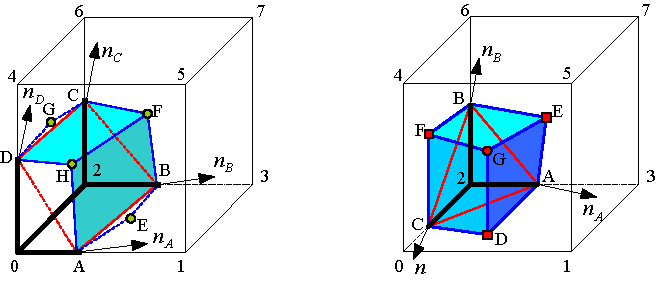
\includegraphics[width=0.9\textwidth]{images/tri_dexel_refinement}
	\caption{
		Triangulating a tri-dexel cell's boundary loops with additional feature information \cite{tridexel_reconstruction}.
		The left image shows the creation of two intermediate vertices, F and H.
		The right image shows the creation of three intermediate vertices, D, E and F, and an apex vertex, G.
	}
	\label{fig:tri_dexel_refinement}
\end{figure}
%
All feature points are calculated using the intersection of three planes.
For the intermediate vertices between two adjacent loop vertices, two planes are given by the two vertices' normals and one plane is given by the cell's side containing both vertices.

In the left drawing of figure \ref{fig:tri_dexel_refinement}, the original boundary loop consists of the vertices A, B, C, and D.
Each of these points holds an additional normal, $n_A$, $n_B$, $n_C$ and $n_D$.
Now, the intermediate point G for example is calculated from the two planes described by the positions and normals of D and C and the cell side to the left.
Using this scheme, an intermediate vertex is calculated for each adjacent pair of vertices on the boundary loop.
In case the calculated vertex is too close to the original edge or lies outside the cell's bounding box, the vertex is discarded.
The vertices G and E are too close to their edges CD and AB and discarded, whereas vertex H and F are kept.

If at least three intermediate vertices are created, an additional apex vertex may be calculated, again as intersection of three planes.
For these planes, the first three loop vertices are taken, which have resulted in the construction of a valid intermediate vertex.
In the right drawing of figure \ref{fig:tri_dexel_refinement}, the loop vertices A, B and C have resulted in intermediate vertices, namely D, E and F.
The first three of them, A, B, and C, are then used to form three planes which intersect in the apex point G.
The location of the apex is also checked against the cell's bounding box.
In case it is outside, the apex is discarded again.

Finally, after creating intermediate and apex vertices, the enhanced boundary loops must be triangulated.
This task is not as easy as the simple triangulation of a loop, as some cases must be distinguish, depending on the availability of intermediate and apex vertices.
%In case a valid apex vertex has been created, the intermediate vertices are placed between the original loop vertices and the resulting loop is triangulated into a fan with the apex vertex as center.
%Otherwise, if no intermediate vertex is found at all, the initial loop is just triangulated into a fan with its center of mass as center, \cf \textproc{TriangulateLoopSimple}.
%If one intermediate vertex is found, the loop is triangulated with the intermediate vertex as center.
%If more than one intermediate vertex is found, the loop is split into subloops.
%Each sequence of an intermediate vertex, an arbitrary number of original loop vertices and another intermediate vertex is triangulated.
%This loop clipping is repeated until only one loop with intermediate vertices is left, which is also triangulated.

Algorithm \ref{alg:tri_dexel_refinement} describes the details of the refinement and feature reconstruction pass, creating enhanced boundary loops for triangulation.
This algorithm acts as a replacement for the \textproc{TriangulateLoopSimple} function of algorithm \ref{alg:tri_dexel_triangulation}.
%
\begin{algorithm}
	\centering
	\begin{algorithmic}[1]
		\Function{TriangulateLoopRefined}{$\var{loop}, \var{cell}$}
			\State $\var{inside} \gets \var{p} \rightarrow \var{cell}.\var{aabb}.\var{lower} < \var{p} < \var{cell}.\var{aabb}.\var{upper}$
			\State $\var{apexVertices} \gets \var{array}()$
			\State $\var{finalLoop} \gets \var{array}()$
			\State $\var{isEdgeVertex} \gets \var{array}()$
			\State $\var{intermedCount} = 0$
			\LineComment{Create new boundary loop with intermediate vertices}
			\For{$\var{i} \gets 0 \To |\var{loop}| - 1$}
				\State $\var{a} \gets \var{loop}_{\var{i}}$
				\State $\var{b} \gets \var{loop}_{(\var{i} + 1) \mod |\var{loop}|}$
				\State $\var{finalLoop}.\var{add}(\var{a}.\var{position})$
				\State $\var{isEdgeVertex}.\var{add}(\True)$
				\State $\var{points} \gets \Call{Unique}{(\var{a}.\var{point}, \var{a}.\var{neigbor}, \var{b}.\var{point}, \var{b}.\var{neighbor})}$
				\State $\var{n} \gets \var{cellSideNormals}_{\var{points}_0, \var{points}_1, \var{points}_2}$
				\State $\var{cellPlane} \gets \var{Plane}(\var{n}, \var{cell}.\var{realPoints}_{\var{points}_0})$
				\State $\var{aPlane} \gets \var{Plane}(\var{a}.\var{normal}, \var{a}.\var{position})$
				\State $\var{bPlane} \gets \var{Plane}(\var{b}.\var{normal}, \var{b}.\var{position})$
				\State $\var{intermed} \gets \Call{IntersectPlanes}{\var{cellPlane}, \var{aPlane}, \var{bPlane}}$
				\If{$\var{intermed} \wedge \var{inside}(\var{intermediate})$}
					\State $\var{dist} \gets \Call{PointLineDistance}{\var{a}.\var{position}, \var{b}.\var{position}, \var{intermed}}$
					\If{$\var{dist} > \epsilon_{\var{line}}$}
						\State $\var{finalLoop}.\var{add}(\var{intermed})$
						\State $\var{isEdgeVertex}.\var{add}(\False)$
						\State $\var{intermedCount} \gets \var{intermedCount} + 1$
						\State $\var{apexVertices}.\var{add}(\var{a})$
						\State $\var{apexVertices}.\var{add}(\var{b})$
					\EndIf
				\EndIf
			\EndFor
			\LineComment{Try to create an apex vertex}
			\If{$\var{intermedCount} \geq 3$}
				\State $\var{apexVertices} \gets \Call{Unique}{\var{apexVertices}}$
				\State $\var{planes} \gets \var{array}()$
				\For{$\var{i} \gets 0 \To 2$}
					\State $\var{planes}.\var{add}(\var{Plane}(\var{apexVertices}_{\var{i}}.\var{normal}, \var{apexVertices}_{\var{i}}.\var{position}))$
				\EndFor
				\State $\var{a} \gets \Call{IntersectPlanes}{\var{planes}_0, \var{planes}_1, \var{planes}_2}$
				\If{$\var{a} \wedge \var{inside}(\var{a})$}
					\State $\var{apex} \gets \var{a}$
				\EndIf
			\EndIf
			\State $\dots$
		\algstore{refinement}
	\end{algorithmic}
	\caption{
		Refinement, feature reconstruction by calculating intermediate vertices and an optiona apex based on the original boundary loops.
		The algorithm is continued in algorithm \ref{alg:tri_dexel_refinement_triangulation}.
	}
	\label{alg:tri_dexel_refinement}
\end{algorithm}
%
In the beginning, a closure is created to test if a point is inside the bounding box of the passed cell.
Then, a few arrays are created.
One contains a list of vertices which have led to a valid intermediate point and may be considered for creating an apex vertex, called \var{apexVertices}.
The variable \var{finalLoop} will contain the original boundary loop's vertices interleaved with the created intermediate vertices.
The \var{isEdgeVertex} array complements the \var{finalLoop} array, as it stores a Boolean value for each of the vertices in the final loop.
This Boolean value is true if the vertex at the same index originated from an edge of the cell and false if the vertex is an intermediate vertex.
Finally, a counter for the number of successfully created intermediate vertices is created and initialized to zero.
A loop then iterates over all vertices \var{a} and their successors \var{b}, \ie adjacent pairs, of vertices of the original loop.
Vertex \var{a} is added to the final loop and \True to \var{isEdgeVertex}.
Afterwards, the four grid point indices of both edge vertices are collected and uniqued.
As both edge vertices share a common side of the cell, the result is a list of grid point indices with either 4 or 3 elements, depending on whether or not one of them is shared.
Three of these indices uniquely identify one of the cell's sides and are used as indices into another lookup table, \var{cellSideNormals}, storing the cell side's normal for each combination of three grid points.
The normal is retrieved using the first three grid points of the current edge vertex pair and stored in \var{n}.
Now, three planes are created, one using the cell side's normal and the coordinate of a grid point on this cell side and two others from the pair of edge vertices.
By calling \textproc{IntersectPlanes}, the intersection point of the three planes is calculated, which is a possible intermediate vertex.
The returned result in \var{intermed} is tested for validity as \textproc{IntersectPlanes} may return an empty result if no intersection could be found.
Furthermore, the intersection point must lie within the bounds of the cell.
If these conditions are satisfied, the distance from the line between the pair of vertices to the calculated intersection point is measured.
If this distance is larger than a specified and small $\epsilon_{\var{line}}$, the intersection point is accepted as an intermediate vertex.
It is therefore added to the final loop.
As it is not an edge vertex, \False is added to the \var{isEdgeVertex} list.
Furthermore, the intermediate vertex counter is incremented and both edge vertices are added to the list of candidates for apex creation.

After all edge vertex pairs of the initial loop have been processed and all intermediate vertices have been created, an apex vertex may be generated.
Therefore, the number of emitted intermediate vertices is checked.
If this number is larger than or equal to 3, the first 3 unique edge vertices are used to create three planes which are again intersected.
In case an intersection point could be found and it also lies within the cell's bounding box, it is accepted as valid apex vertex.

Now, enough information has been gathered from the normal information at each vertex to begin triangulating the loop.
This second part of the \textproc{TriangulateLoopRefined} function is listed in algorithm \ref{alg:tri_dexel_refinement_triangulation}.
%
\begin{algorithm}
	\centering
	\begin{algorithmic}[1]
		\algrestore{refinement}
			\State $\dots$
			\If{$\var{apex}$}
				\State \Return $\Call{TriangulateLoopIntoFan}{\var{finalLoop}, \var{apex}}$
			\ElsIf{$\var{intermedCount} = 0$}
				\State \Return $\Call{TriangulateLoopIntoFan}{\var{finalLoop}}$
			\ElsIf{$\var{intermedCount} = 1$}
				\State $\Call{Rotate}{\var{finalLoop}, \Call{FindFirst}{\var{isEdgeVertex}, \False}}$
				\State \Return $\Call{TriangulateLoopAtFirst}{\var{finalLoop}}$
			\Else
				\State $\var{triangles} \gets \varnothing$
				\For{$\var{first} \gets 0 \To |\var{finalLoop}| - 1$} \Comment{Reevaluated at each iteration}
					\If{$\neg \var{isEdgeVertex}_{\var{first}}$}
						\State $\var{last} \gets (\var{first} + 1) \mod |\var{finalLoop}|$
						\While{$\var{isEdgeVertex}_{\var{last}}$}
							\State $\var{last} \gets (\var{last} + 1) \mod |\var{finalLoop}|$
						\EndWhile
						\State $\var{subLoop} \gets \var{array}()$
						\For{$\var{i} \gets (\var{first} \To \var{last}) \mod |\var{finalLoop}|$}
							\State $\var{subLoop}.\var{add}(\var{finalLoop}_{\var{i}})$
						\EndFor
						\State $\var{triangles} \gets \var{triangles} \cup \Call{TriangulateLoopIntoFan}{\var{subLoop}}$
						\State $\Call{RemoveCyclicRange}{\var{finalLoop}, \var{first} + 1, \var{last} - 1}$
						\State $\Call{RemoveCyclicRange}{\var{isEdgeVertex}, \var{first} + 1, \var{last} - 1}$
					\EndIf
				\EndFor
				\State $\var{triangles} \gets \var{triangles} \cup \Call{TriangulateLoopIntoFan}{\var{finalLoop}}$
				\State \Return $\var{triangles}$
			\EndIf
		\EndFunction
		\\
		\Function{IntersectPlanes}{$\var{a}, \var{b}, \var{c}$}
			\State $\var{det} \gets \begin{vmatrix} \var{a}.\var{normal} & \var{b}.\var{normal} & \var{c}.\var{normal} \end{vmatrix}$
			\If{$|\var{det}| > \epsilon_{\var{plane}}$}
				\State \Return $((\var{b}.\var{normal} \times \var{c}.\var{normal}) \cdot \var{a}.\var{dist} + {}$\hfill\break
				\hspace*{\dimexpr\algorithmicindent*2}\phantom{\Return $($}$(\var{c}.\var{normal} \times \var{a}.\var{normal}) \cdot \var{b}.\var{dist} + {}$\hfill\break
				\hspace*{\dimexpr\algorithmicindent*2}\phantom{\Return $($}$(\var{a}.\var{normal} \times \var{b}.\var{normal}) \cdot \var{c}.\var{dist}) \div \var{det}$
			\EndIf
			\LineComment{Otherwise, return nothing}
		\EndFunction
		\\
		\Function{PointLineDistance}{$\var{a}, \var{b}, \var{p}$}
			\State \Return $|(\var{p} - \var{a}) \times (\var{p} - \var{b})| \div |\var{a} - \var{b}|$
		\EndFunction
	\end{algorithmic}
	\caption{
		Continuation of algorithm \ref{alg:tri_dexel_refinement}.
		Triangulation of a boundary loop enhanced with intermediate vertices and an optional apex.
	}
	\label{alg:tri_dexel_refinement_triangulation}
\end{algorithm}
%
For the triangulation of the loop, enriched with intermediate vertices and an optional apex vertex, several cases have to be distinguished, depending on the available data.

If an apex vertex has been found, the final loop containing edge and intermediate vertices is directly triangulated into a fan with the apex vertex as center.

If no apex and intermediate vertices have been found, the loop is triangulated the same way as in the \textproc{TriangulateLoopSimple} version, by creating a fan around the loops centroid.

If no apex and one intermediate vertex are found, the loop is triangulated as a fan around the intermediate vertex.
Therefore, the loop is rotated to start with the intermediate vertex and then passed to \textproc{TriangulateLoopAtFirst}.

Loops with no apex vertex and more than one intermediate vertex are more difficult to triangulate.
The case illustrated in figure \ref{fig:tri_dexel_refinement} on the left shows that the final loop must actually split into two sub loops, one containing C, D, H and F, as well as one containing A, B, D, H.
This fact becomes even clearer with cases like the one on the right if the apex vertex was invalid, \eg the apex G would be outside the cell's box.
In this case, all intermediate vertices D, E and F would form a plateau.
The remaining parts of the final loop are sub loops, each consisting of two neighboring intermediate vertices and the edge vertices in-between.

This sub loop clipping strategy is now algorithmically applied to \var{finalLoop}.
A for loop iterates over the indices of all vertices, each the first element of a potential sub loop.
If the vertex at this current index is not an edge vertex, \ie an intermediate vertex, then a nested loop searches the next, cyclically occurring intermediate vertex on the loop, skipping all edge vertices in between.
After it has been found, the inclusive range from \var{first} to \var{last} contains a sub loop, which is now copied from \var{finalLoop} and triangulated into a fan.
Afterwards, the sub loop's edge vertices are removed from \var{finalLoop} and \var{isEdgeVertex}.
After all such sub loops have been clipped and triangulated, \var{finalLoop} consists only of intermediate vertices.
These are also triangulated.
The union of the triangulations of all sub loops and the remaining final loop forms the triangulation of the complete boundary loop and is returned.

Throughout the \textproc{TriangulateLoopRefined} function, two helper functions are used.
The first, \textproc{IntersectPlanes}, calculates the intersection point between three planes.
A good algorithm for this problem is found in the Graphics Gems series \cite[p304]{graphics_gems_1}.
It describes the intersection point as the solution of a system of linear equations as follows:
For three planes with normals $n_a$, $n_b$, $n_c$ and distances $d_a$, $d_b$, $d_c$, intersecting at $x$, $y$, $z$, using the variables
\begin{equation}
	N = \begin{bmatrix} n_a, n_b, n_c \end{bmatrix}, \;
	I = \begin{bmatrix} x \\ y \\ z \end{bmatrix}, \;
	d = \begin{bmatrix} d_a \\ d_b \\ d_c \end{bmatrix},
\end{equation}
the system
\begin{equation}
N I = d
\end{equation}
is solved using Cramer's rule
\begin{equation}
	x = \frac{\begin{vmatrix} d, n_b, n_c \end{vmatrix}}{|N|}, \;
	y = \frac{\begin{vmatrix} n_a, d, n_c \end{vmatrix}}{|N|}, \;
	z = \frac{\begin{vmatrix} n_a, n_b, d \end{vmatrix}}{|N|} \text{.}
\end{equation}
By describing the intersection point as
\begin{equation}
	I =
	x \begin{bmatrix} 1 \\ 0 \\ 0 \end{bmatrix} +
	y \begin{bmatrix} 0 \\ 1 \\ 0 \end{bmatrix} +
	z \begin{bmatrix} 0 \\ 0 \\ 1 \end{bmatrix} \text{,}
\end{equation}
substituting $x$, $y$ and $z$ and expanding the determinant into a triple product, the equation becomes
\begin{equation}
	I =
	\frac{d \times n_b \cdot n_c}{|N|} \begin{bmatrix} 1 \\ 0 \\ 0 \end{bmatrix} +
	\frac{n_a \times d \cdot n_c}{|N|} \begin{bmatrix} 0 \\ 1 \\ 0 \end{bmatrix} +
	\frac{n_a \times n_b \cdot d}{|N|} \begin{bmatrix} 0 \\ 0 \\ 1 \end{bmatrix} \text{.}
\end{equation}
As the operands of the triple product can be rotated, $d$ is isolated from the cross product.
Then, the vectors after the fractions are lifted onto the numerator and multiplied with $d$, extracting the components $d_a$, $d_b$ and $d_c$, resulting in
\begin{equation}
I =
	\frac{n_b \times n_c \cdot d_a}{|N|} +
	\frac{n_c \times n_a \cdot d_b}{|N|} +
	\frac{n_a \times n_b \cdot d_c}{|N|} \text{.}
\end{equation}
By combining all three fractions, the equation for the intersection calculation, which is used by the \textproc{IntersectPlanes} function, is complete.
If the determinant of matrix $N$ becomes zero, two of the contained normal vectors and therefore planes are parallel.
Determinants close to zero, \ie smaller than $\epsilon_{\var{plane}}$, may further cause numeric issues when calculating the intersection point.
Therefore, in this case, the function does not return a result, \ie a result which always evaluates to \False in Boolean expressions.

The function \textproc{PointLineDistance} computes the closest distance of a point \var{p} to the line defined by two other points \var{a} and \var{b}.
The implemented variant to solve this problem \cite{point_line_distance}, computes the length of the cross product between the two vectors from \var{p} to both line endings.
This value is the doubled area of the triangle \var{a}, \var{b}, \var{c}, where the line distance is the altitude of the triangle.
Dividing the doubled area by the triangle's base, \ie the length of the line $\overline{\var{a}\var{b}}$, the point to line distance is obtained.


\subsection{Cell slicing}
\label{sec:tri_dexel_cellslicing}

With the additional refinement and feature reconstruction introduced in section \ref{sec:tri_dexel_refinement}, the quality of the tri-dexel surface reconstruction is improved appreciably.
Still, features within a cell and especially thin features not crossing any grid points are almost fully discarded.
The reason therefore is the the destructive regularization step described in section \ref{sec:tri_dexel_regularization}, which sacrifices smaller dexel segments in favor of regularity, throwing away useful information, especially of smaller features.
To preserve this information and still obtain regular tri-dexel cells, which can be passed into the triangulation routines of sections \ref{sec:tri_dexel_triangulation} and \ref{sec:tri_dexel_refinement}, an alternative to the regularization algorithm has been developed.
This novel approach depends on the ability to resample dexels at any time, an ability usually not given in scenarios where the dexel model is the main data model, \ie typical, dexel-based machining simulations.
However, as the dexel model used for surface reconstruction is derived from the VML's internal data model, it allows to arbitrarily recreate dexels.

\begin{figure}
	\centering
	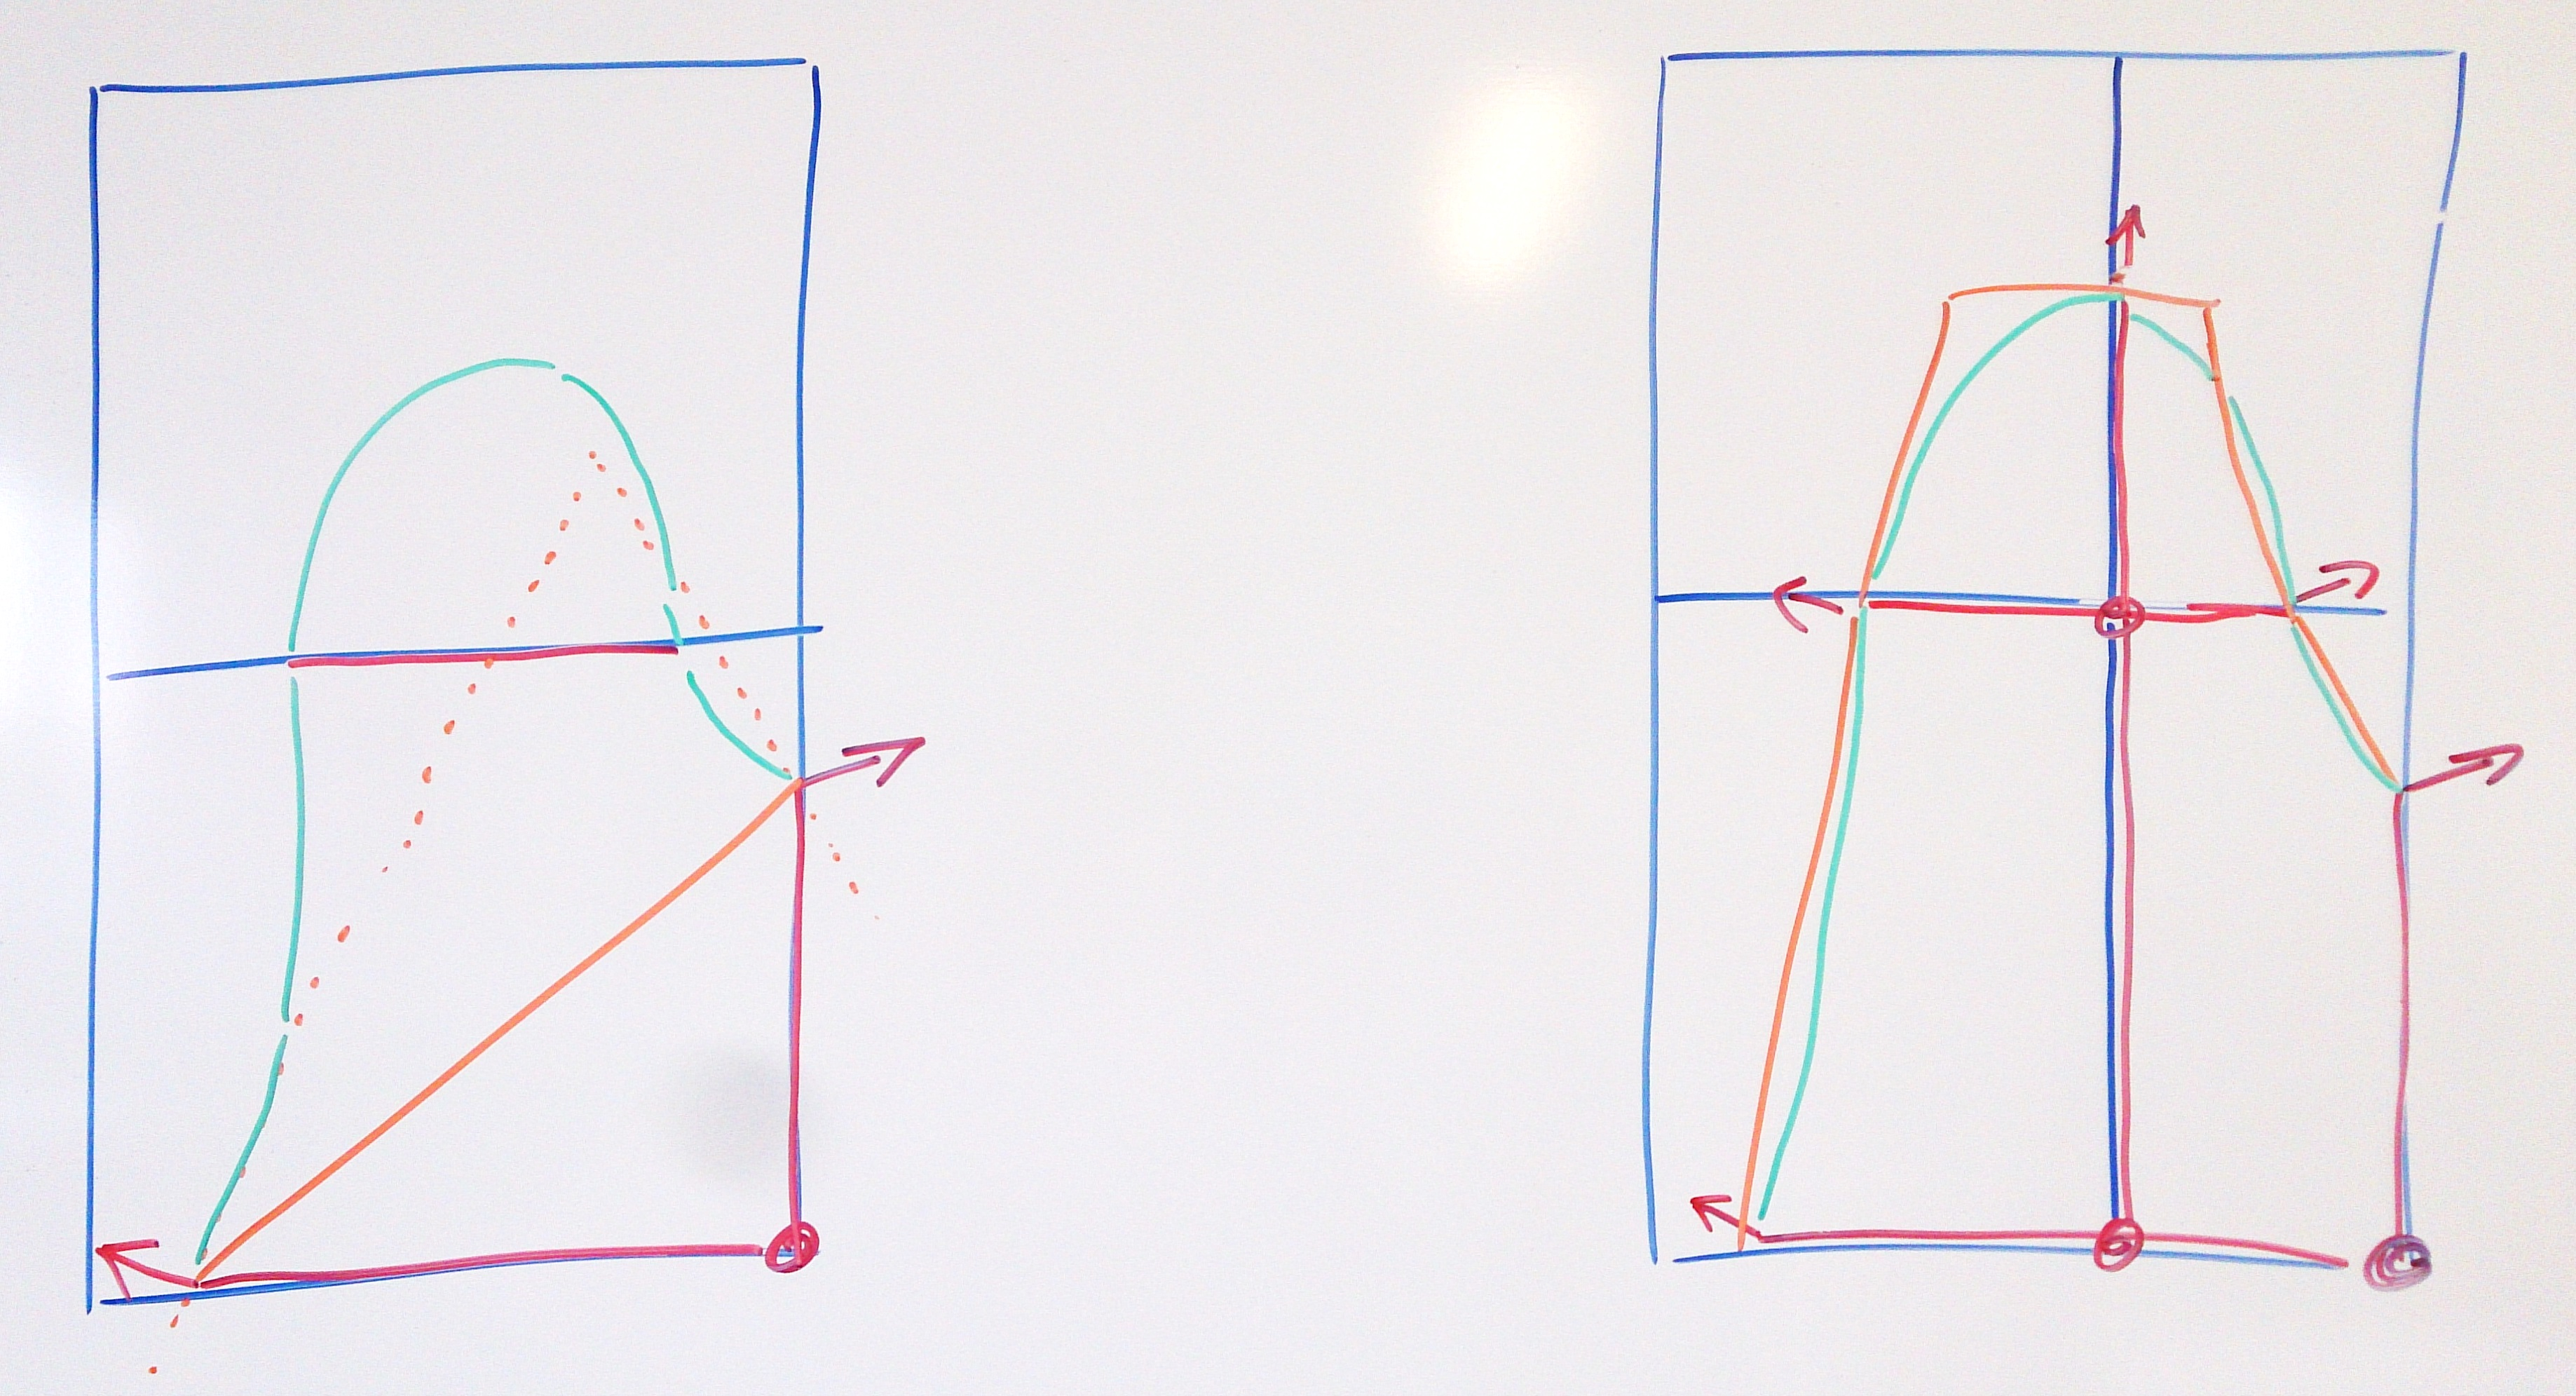
\includegraphics[width=0.7\textwidth]{images/tri_dexel_cellslicing}
	\caption{
		Creating regular cells by slicing two irregular cells sharing an irregular edge.
		The actual surface is drawn in green, the reconstructed one in red.
		A possible intermediate vertex in the left scenario is discarded, as it is outside the cell's bounding box.
	}
	\label{fig:tri_dexel_cellslicing}
\end{figure}

The main problem of small dexel segments is that they are always lost during regularization if they do not pass a grid point of the tri-dexel grid.
If a lot of fine features are shed this way, an obvious solution is to increase the resolution of the dexel grid.
However, this solution dramatically increases memory and computational demands and also adds detail where it is not necessary, \eg in large flat surfaces or empty space.
A more elegant solution is to increase the grid resolution locally.
More specifically, each irregular cell, \ie a cell which contains irregular edges, \ie edges which have to be modified by the regularization, is subdivided in such a way that all irregular edges become regular, without modifying the segments.
This subdivision is accomplished by calculating divider planes for each irregular cell.
As much planes as necessary are created to slice all segments or empty spaces between segments, which would be discarded by the regularization.
Figure \ref{fig:tri_dexel_cellslicing} shows this procedure by an example.
The left drawing shows a small feature which will be lost due to regularization as the edge shared by both cells is irregular; regularization rule 2 will remove the segment.
As the calculated intermediate point lies outside the lower cell, \cf dotted lines in red, the quality of the reconstructed surface is poor.
The right image shows the same situation with an additional divider line (plane in 3D).
The divider is resampled, creating new dexel segments.
All resulting 4 cells are now regular and, after triangulation, produce a good surface approximation.

Nevertheless, after slicing irregular cells to ensure regularity on the edges, the resampled dexels within the cell might again produce irregular cells.
Therefore, this cell slicing technique is applied recursively.
As the detail of the reconstructed surface is increased on each subdivision at the cost of more and finer triangles, the use of a maximum recursion depth is advised.
When this limit is hit, the cell, despite being irregular, is passed to the standard regularization algorithm, discarding the now hopefully expendable features.

\begin{figure}
	\centering
	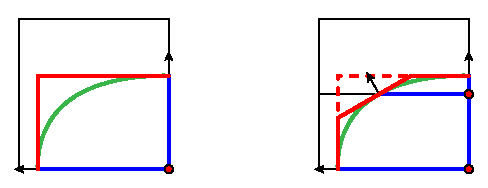
\includegraphics[width=0.9\textwidth]{images/tri_dexel_hole_creation}
	\caption{
		Creating a hole at the border of a normal and a sliced cell by estimating different feature points.
		The original surface is drawn in green, the reconstructed one in red.
	}
	\label{fig:tri_dexel_hole_creation}
\end{figure}

Adaptively slicing cells and resampling the model to a higher level of detail in distinct places is dangerous and may create thin holes on the surface.
The tri-dexel reconstruction algorithm usually generates a closed manifold by assuming that the same feature points and edges are created by two adjacent cells at their common border.
If one of the cells is sliced, feature points might be estimated differently.
Figure \ref{fig:tri_dexel_hole_creation} shows an example of a case where a hole is created between a normal and a sliced cell.
The sketch on the left shows a cell side estimating a feature point based on the dexel segments at the cell's edges.
The sketch on the right shows the adjacent cell's side, which has been sliced, \eg by another irregular edge at the opposite cell side.
Due to the additional information gathered by the resampled dexel at the slicing plane, two feature points are calculated in the sliced cell, instead of one in the unsliced cell.
Thus, a different surface is created at the border, resulting in a typically thin hole.

The cells resulting from slicing are resampled, regularized and triangulated by reusing all existing classes and algorithms.
For each cell a new tri-dexel image is created with a resolution of 2 in each dimension with exactly the same bounding box as the cell.
The reconstruction proceeds analogously to the one of the main tri-dexel image, \cf algorithm \ref{alg:tri_dexel} line \ref{alg:line:tri_dexel_begin}ff. %TODO

This new cell slicing algorithm is integrated into the existing code by adapting the base tri-dexel reconstruction algorithm, algorithm \ref{alg:tri_dexel}, as shown in algorithm \ref{alg:tri_dexel_2}.
%
\begin{algorithm}
	\centering
	\begin{algorithmic}[1]
		\setalglineno{6}
		\Function{Reconstruct}{$grid, box, resolution$}\hfill\break
			\hspace*{\dimexpr\algorithmicindent*1}\dots
			\setalglineno{11}
			\ForAll{$\var{cell} \in \var{dgrid}.\var{cells}()$}
				\If{$\Call{RegularizeCell}{\var{cell}, \True}$}
					\State $\var{triangles} \gets \var{triangles} \cup \Call{TriangulateCell}{\var{cell}}$
				\Else
					\State $\var{triangles} \gets \var{triangles} \cup \Call{SliceCell}{\var{cell}, \var{grid}}$
				\EndIf
			\EndFor
			\State \Return $\var{triangles}$
		\EndFunction
	\end{algorithmic}
	\caption{
		Adaption to the abstract workflow given in algorithm \ref{alg:tri_dexel} to support cell slicing.
	}
	\label{alg:tri_dexel_2}
\end{algorithm}
%
The \textproc{RegularizeCell} procedure is slightly adapted.
A Boolean value is added to its interface and, if cell slicing is allowed, a value \True is passed to \textproc{RegularizeCell}, indicating that only numeric regularizations, \cf regularization rule 3, are allowed and other necessary regularizations, \ie irregular edges, are only detected but not applied.
A Boolean return value of \textproc{RegularizeCell} informs the if irregular edges have been detected.
In this case, the cell is not sent to triangulation but to a new cell slicing algorithm, the \textproc{SliceCell} function.

\begin{algorithm}
	\centering
	\begin{algorithmic}[1]
		\Function{SliceCell}{$\var{cell}, \var{grid}$}
			\State $(\var{xdiv}, \var{ydiv}, \var{zdiv}) \gets \Call{FindDividers}{\var{cell}}$
			\State $\var{triangles} \gets \varnothing$
			\ForAll{$\var{x} \gets 0 \To |\var{xdiv}| - 2, \var{y} \gets 0 \To |\var{ydiv}| - 2, \var{z} \gets 0 \To |\var{zdiv}| - 2$}
				\State $\var{lower} \gets \var{Vertex}(\var{xdiv}_{\var{x}    }, \var{ydiv}_{\var{y}    }, \var{zdiv}_{\var{z}    })$
				\State $\var{upper} \gets \var{Vertex}(\var{xdiv}_{\var{x} + 1}, \var{ydiv}_{\var{y} + 1}, \var{zdiv}_{\var{z} + 1})$
				\State $\var{box} \gets \var{Extends}(\var{lower}, \var{upper})$
				\State $\var{triangles} \gets \var{triangles} \cup \Call{Reconstruct}{\var{grid}, \var{box}, (2, 2, 2)}$
			\EndFor
			\State \Return $\var{triangles}$
		\EndFunction
		\\
		\Function{FindDividers}{$\var{cell}$}
			\State $\var{axisRanges} \gets \var{array}(3, \var{array}())$
			\For{$ \var{i} \gets 0 \To 11 $}
				\State $\dots$ \Comment{Same vars as in regularization, algorithm \ref{alg:tri_dexel_regularization}, line \ref{alg:line:reg_vars_begin} to \ref{alg:line:reg_vars_end}}
				\If{$(\var{srcOcc} \wedge \var{dstOcc} \wedge |\var{segs}| > 1) \vee {}$\hfill\break
					\hspace*{\dimexpr\algorithmicindent*3}$(\neg \var{srcOcc} \wedge \neg \var{dstOcc} \wedge |\var{segs}| > 0) \vee {}$\hfill\break
					\hspace*{\dimexpr\algorithmicindent*3}$ (\var{srcOcc} \neq \var{dstOcc} \wedge |\var{segs}| > 1)$}
					\State $\var{axisRanges}_{\var{axis}}.\var{add}(\Call{SegmentsToRanges}{\var{segs}, \var{srcDepth}, \var{dstDepth}})$
				\EndIf
			\EndFor
			\State $\var{dividers} \gets array(3, \var{array}())$
			\For{$\var{axis} \gets 0 \To 2$}
				\State $\var{ranges} \gets \Call{Sort}{\var{axisRanges}_{\var{axis}}}$ \Comment{Sort by range start}
				\State $\var{dividers}_{\var{axis}}.\var{add}(\var{cell}.\var{aabb}.\var{lower}_{\var{axis}})$
				\State $(\var{start}, \var{end}) \gets \var{ranges}_0$
				\For{$\var{i} \gets 1 \To |\var{ranges}| - 1$}
					\If{${\var{ranges}_{\var{i}}}_0 > \var{end}$}
						\State $\var{dividers}_{\var{axis}}.\var{add}((\var{start} + \var{end}) \div 2)$
						\State $(\var{start}, \var{end}) \gets \var{ranges}_{\var{i}}$
					\Else
						\State $\var{start} \gets {\var{ranges}_{\var{i}}}_0$
						\State $\var{end} \gets \Call{Min}{\var{end}, {\var{ranges}_{\var{i}}}_1}$
					\EndIf
				\EndFor
				\State $\var{dividers}_{\var{axis}}.\var{add}((\var{start} + \var{end}) \div 2)$
				\State $\var{dividers}_{\var{axis}}.\var{add}(\var{cell}.\var{aabb}.\var{upper}_{\var{axis}})$
			\EndFor
			\State \Return $\var{dividers}$
		\EndFunction
		\\
		\Function{SegmentsToRanges}{$\var{segs}, \var{srcDepth}, \var{dstDepth}$}
			\State $\var{depths} \gets \var{array}()$
			\ForAll{$\var{seg} \in \var{segs}$}
				\If{$\var{seg}.\var{start}.\var{depth} \neq \var{srcDepth}$}
					$\var{depths}.\var{add}(\var{seg}.\var{start}.\var{depth})$
				\EndIf
				\If{$\var{seg}.\var{end}.\var{depth} \neq \var{dstDepth}$}
					$\var{depths}.\var{add}(\var{seg}.\var{end}.\var{depth})$
				\EndIf
			\EndFor
			\State $\var{ranges} \gets \var{array}()$
			\For{$\var{i} \gets 0 \To |\var{depths}| - 2$}
				\State $\var{ranges}.\var{add}((\var{depths}_{\var{i}}, \var{depths}_{\var{i} + 1}))$
			\EndFor
			\State \Return $\var{ranges}$
		\EndFunction
	\end{algorithmic}
	\caption{
		Cell slicing algorithm.
		The \textproc{SliceCell} function is indirectly recursive with \textproc{Reconstruct}.
	}
	\label{alg:tri_dexel_cell_slicing}
\end{algorithm}

Given in algorithm \ref{alg:tri_dexel_cell_slicing}, cell slicing starts by finding axis aligned divider planes along the x-, y- and z-axis.
Each list of dividers along one axis starts with the depth of the corresponding source grid points, then contains a list of depths along the edges of that axis, and then finally contains the depth of the destination grid points, \cf \var{srcDepth} and \var{dstDepth} in \textproc{RegularizeCell}.
Afterwards, the Cartesian product between the dividers of each axis, except the last one, is formed.
Each tuple in this product forms the lower point of a bounding box, the succeeding divider on each axis the upper point.
This way, the loop enumerates all bounding boxes of the sub cells resulting from slicing the cell at all dividers.
These boxes are then used to launch subsequent tri-dexel reconstructions, by recursively calling \textproc{Reconstruct} with the bounding box becoming the new size of the tri-dexel image and grid with a resolution of 2 in each dimension.

\begin{figure}
	\centering
	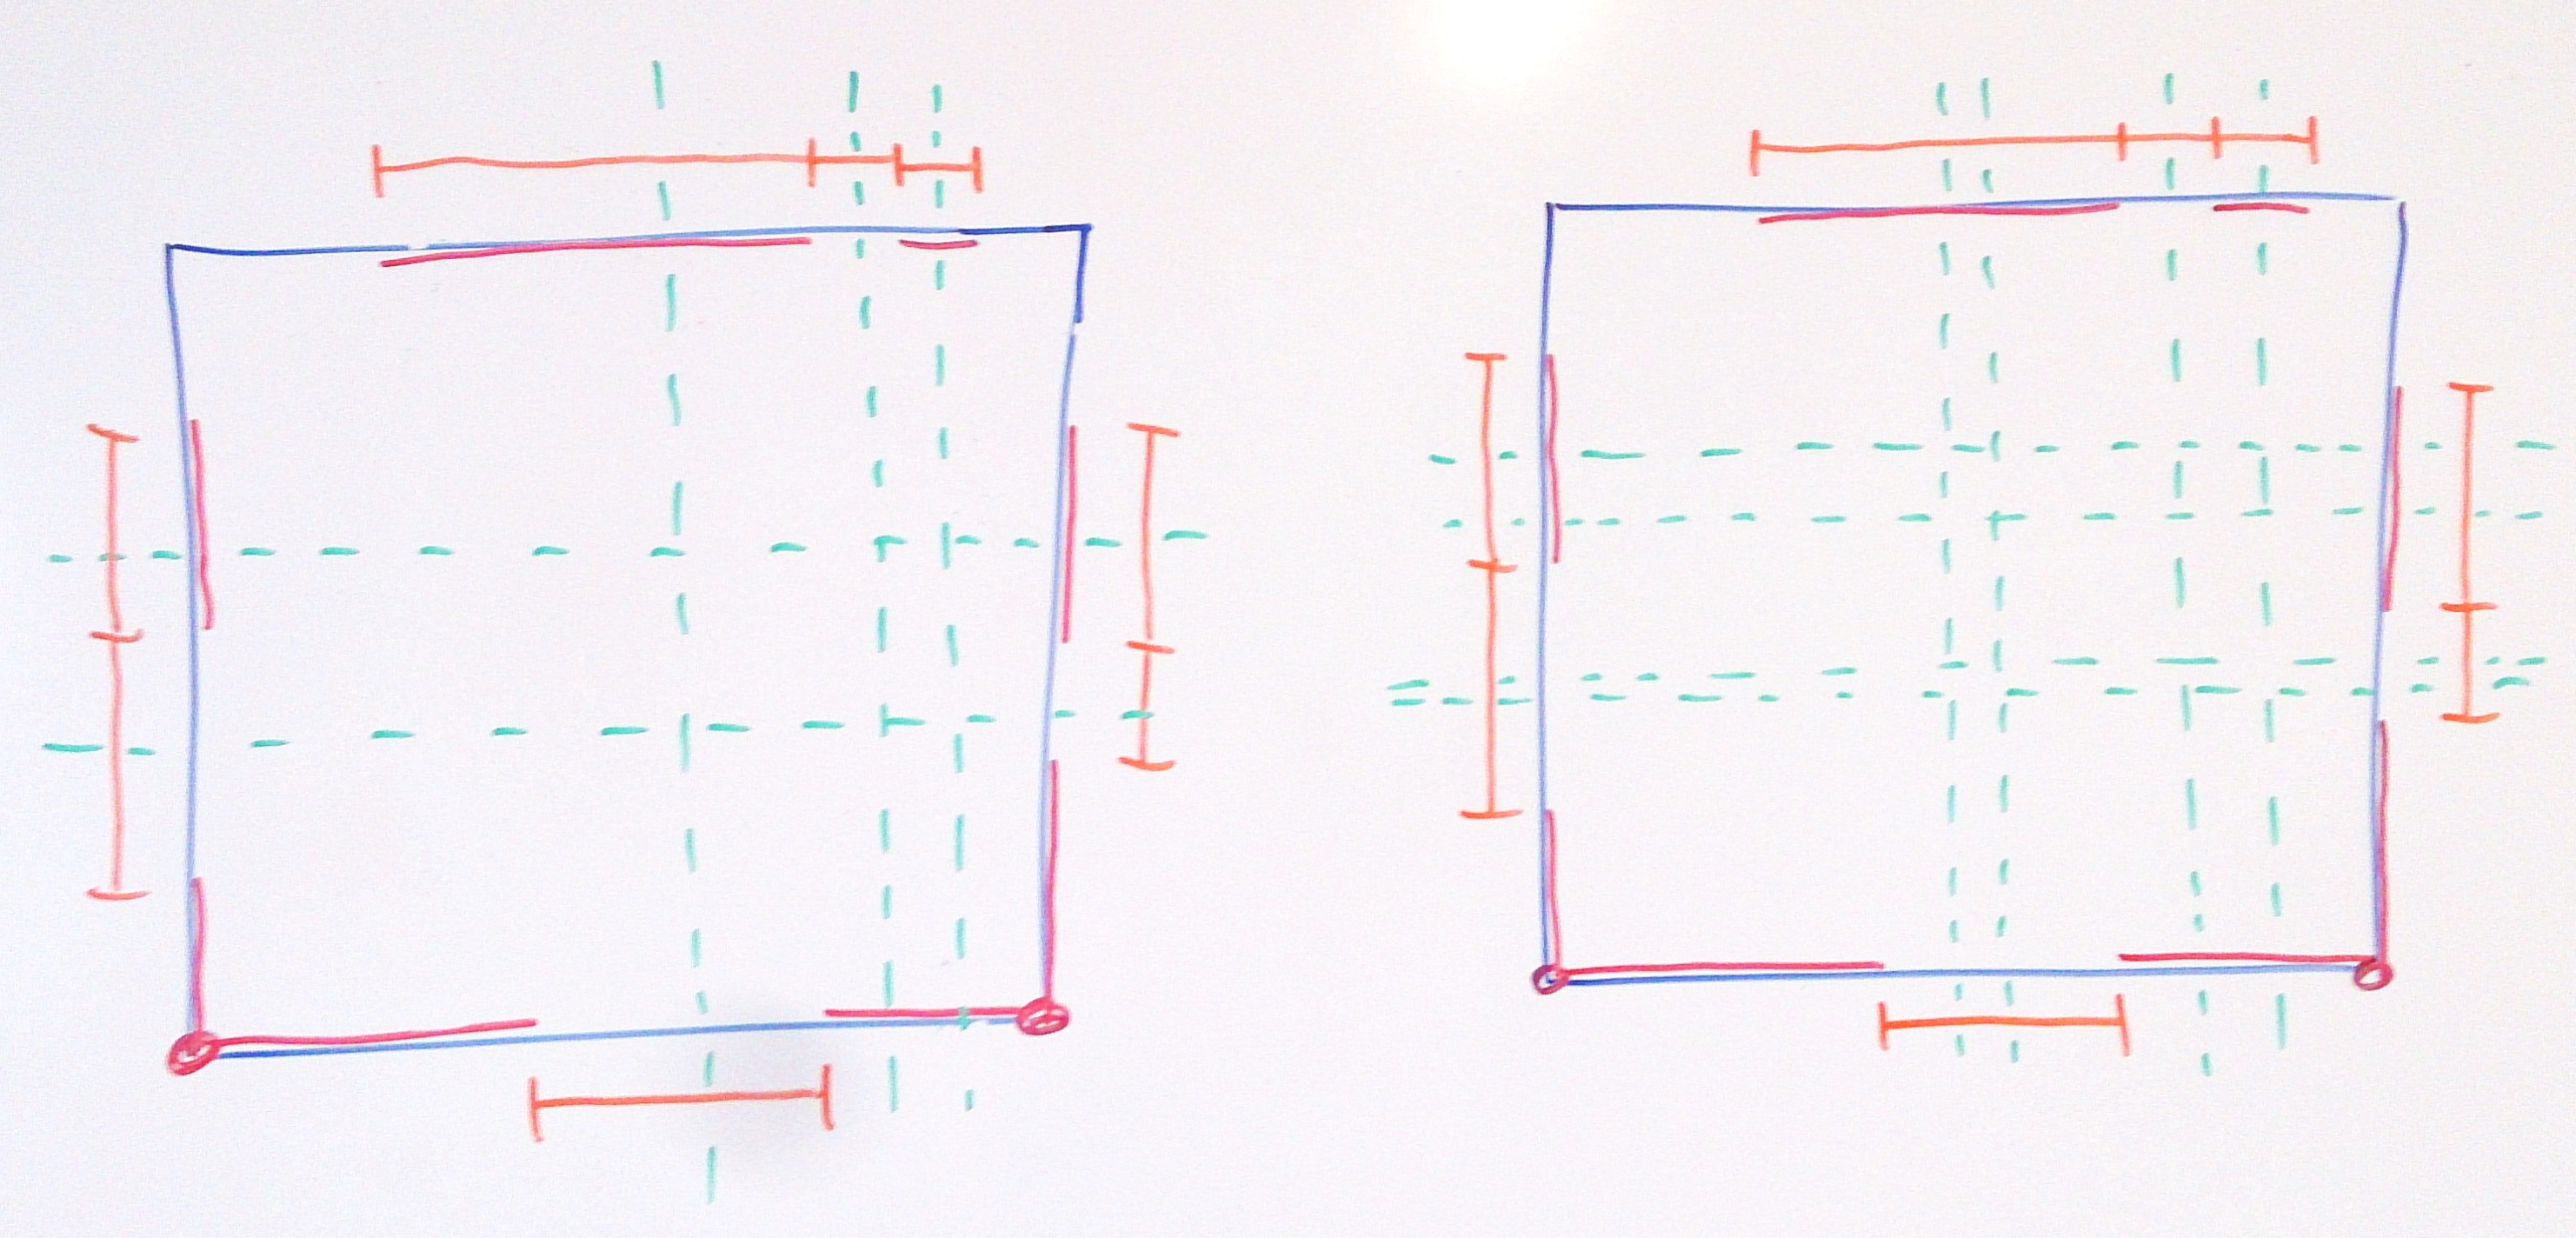
\includegraphics[width=0.9\textwidth]{images/cellslicing_dividers}
	\caption{
		Setting divider planes to slice the ranges derived from the dexel segments and the space between them.
		Segments are blue, ranges in orange, dividers in dotted green lines.
		On the left drawing, dividers are set using an algorithm reducing the total number of dividers needed.
		On the right drawing, a divider is set at the midpoint of each range, resulting in more dividers but maintaining consistency with neighboring cells.
	}
	\label{fig:cellslicing_dividers}
\end{figure}

Most of the work when slicing cells is done in the \textproc{FindDiviers} function, which computes depth values for axis aligned planes along which an irregular cell should be sliced.
The function consists of two steps.
The first is to define depth ranges along each axis which have to be split.
These ranges are basically dexel segments as well as the space between two segments.
Secondly, each of this ranges has to be split by at least one divider plane.
Figure \ref{fig:cellslicing_dividers} illustrates these steps on a cell with calculated depth ranges in orange and two possible divider configurations in green.

The depth ranges are computed for each axis, by iterating over all 12 edges of the cell and computing the same variables as in the regularization algorithm \ref{alg:tri_dexel_regularization}, line \ref{alg:line:reg_vars_begin} to \ref{alg:line:reg_vars_end}.
Using these variables, the algorithm checks if the current edge is irregular, which is the case
\begin{itemize}
	\item if both grid points are occupied and more than one segment is present,
	\item if both grid points are non-occupied and any segment is present,
	\item or, if only one of the grid points is occupied and more than one segment is present.
\end{itemize}
The segments of each irregular edge are then passed to the \textproc{SegmentsToRanges} function, which determines the depth ranges which have to be sliced, and stored for the current axis.

After all depth ranges have been computed, dividers are calculated.
There are multiple possibilities for setting dividers.
Two variations are given in figure \ref{fig:cellslicing_dividers}.
The first one tries to collect as many ranges as possible which are able to be sliced by the same divider.
The second one just creates a divider at the midpoint of each range.
Whereas the first method creates fewer dividers and therefore fewer sub cells which have to be reprocessed, the second one is consistent across neighboring cells as two cells attached to the same irregular edge will create the same dividers.

In algorithm \ref{alg:tri_dexel_cell_slicing}, the first method is implemented as it produces overall better results.
Dividers are computed per axis from the list of ranges found for the current axis, sorted by the ranges' start.
On each axis, the first divider is the bounding box itself, \ie the component of the box's lower vertex corresponding to the current axis.
Then, an interval $(\var{start}, \var{end})$ is set to the first range, indicating a range of possible dividers.
This interval is now iteratively adapted/narrowed to span as many ranges as possible.
For this purpose, a loop iterates over all remaining ranges.
If the start of the current range does exceed the current interval, \ie the range's start is larger than the interval's end, a divider is created for the current interval and the interval reset to the current range.
If the current range does not exceed the current interval, \ie the range's start lies within the interval, it is narrowed by moving its start to the start of the current range.
The end of the current interval is also adapted.
After looping over all ranges has completed, a further divider is also calculated for the remaining interval.
Finally, the bounding box's upper vertex is used to create a last divider.
After the dividers have been calculated for each axis, they are returned to and used for creating the bounding boxes of sub cells.

The \textproc{SegmentsToRanges} function is a simple selector and translator of dexel segments and their space between them.
The algorithm creates the ranges on each axis which must be sliced, \ie for which a divider has to be created.
In order to do so all segments of an edge are flattened into a list of start and end depth values, except values which are at the cell's border, \ie equal to \var{srcDepth} or \var{dstDepth}.
Then, each pair of neighboring depth values are grouped into a tuple, creating a list of depth ranges.
These ranges are shown in orange in figure \ref{fig:cellslicing_dividers} and returned at the end of the function.


\subsection{Parallelization}
\label{sec:tri_dexel_parallelization}

The tri-dexel surface reconstruction algorithm shown in this chapter consists of a number of steps.
The first one is the creation of a tri-dexel image by raycasting the VML's data model.
The size of the tri-dexel image and therefore the number of created rays is parameterized by the user.
Typical resolutions range from 50 for quick approximations up to several hundred\footnote{Resolutions of up to 600 were successfully tested before hitting the \SI{16}{\gibi\byte} physical RAM limit on the used machine.} for fine and detailed reconstructions.
As the number of created rays for a cubic grid with a resolution of $n$ is $3n^2$ and the ray traversal and intersection is perfectly isolated, parallelization of the raycast is embarrassingly simple and usually yields a high number of independent work items.

Concerning the implementation, all 3 for loops in algorithm \ref{alg:tri_dexel_raycast} are viable candidates for parallel execution.
These are the loop iterating over the three coordinate system axes as well as the loops enumerating all ray origins.
Note that the closure called for each hit, \var{hitFunc}, is invoked concurrently.
However, as the number of required dexels is derived from the user specified resolution, the tri-dexel image can preallocate all space required for the raycast result, except the list of nodes per dexel, allowing parallel access.
As a single dexel is only filled by a single ray, no concurrent access occurs on the dynamically resizing dexel lists.

The efficiency of the raycast could be furthered pushed by vectorization or GPU acceleration.
Both of these techniques have been implemented for the raycast used for visualization, \cf section \ref{sec:raycasting}.
However, as the consistency of the dexel image is regarded more important than the speed of its creation, a considerable amount of additional correction code has been added to the raycast.
This code complicates vectorization and GPU acceleration, especially as the latter still does not support dynamic memory allocation on every platform\footnote{CUDA offers malloc in kernels, OpenCL has no equivalent.}.
Furthermore, the list of dexel nodes is a dynamic data structure and filled differently by each ray/thread/work item leading to even more complex vector code or branch divergence on GPUs.

After the raycast, when the creation of the tri-dexel image has completed, the tri-dexel grid is built by assigning all cell edges and grid point occupancies.
This task is also embarrassingly parallel at dexel level.
Considering algorithm \ref{alg:tri_dexel_grid_generation}, the outer three for loops, iterating over the three axes and then over all dexels, are almost completely independent and offer good parallelization candidates.
Assigning the segments on each dexel in parallel is also possible, but requires concurrent segment insertion at a cell edge to be safely, \cf line \ref{alg:line:grid_edge_insertion}.
If the outmost loop on the three axes is parallelized, note that the grid point occupancies are then written concurrently as the occupancy of a single grid point is determined by one dexel from each axis image.
This race condition might not be a problem on some architectures, as the same value, \True, is written concurrently to the same memory location.
However, the result depends on several hardware parameters and the memory model of the language.
For portable consistency, either the outmost loop on the axes must be serial, or the writes to the grid point occupancies atomic.

After the tri-dexel grid has been constructed, all cells have to be processed.
The required algorithms, \ie regularization, triangulation and slicing, operate independently on each cell and may therefore run in parallel.
However, the information a cell contains, \ie grid point occupancies and segments on edges, is shared between neighboring cells.
Algorithms modifying a cells data are therefore subject to race conditions.
This mainly concerns the regularization which changes the segments on cell edges.
Several solutions are available to mitigate this issue.
One possibility is locking a cell's edge during regularization.
Neighboring cells regularized later would then see this edge as already regularized.
Unfortunately, this solution does not work well with the detection of irregular edges and cell slicing strategy, where cells are intentionally kept irregular during regularization.
Furthermore, a huge amount of locks, $\mathcal{O}(n^3)$, would be necessary, putting pressure on the operating system kernel.
A lock-free implementation of the edge's data structure and regularization rules using atomic operations might be possible, but is probably highly difficult to achieve.
A more pragmatic solution, which has been implemented, is to just copy the data of each cell out of the tri-dexel grid before sending a cell to the regularization and subsequent algorithms.
This allows fully independent cell processing, enabling the loop on all cells in \textproc{Reconstruct} in algorithm \ref{alg:tri_dexel} to run in parallel.

The following algorithms still offer a bit of parallelism.
However, as the independent processing of each cell already offers enough work items to saturate a large number of cores, further, nested parallelism is probably unneeded.
Nevertheless, for completeness, they are mentioned shortly.
The regularization of a cell immediately boils down to regularizing all 12 edges of the cell.
These might be regularized in parallel.
The \textproc{FindLoops} routine starting the depth-first searches on the cell might run its 8 searches in parallel, accumulating the loops on a concurrent data structure.
These loops might then also be triangulated in parallel in \textproc{TriangulateCell}.
Intermediate point calculation during refinement on each vertex pair of a loop might also be done in parallel, but is probably not worth the overhead.


\section{Results}
\label{sec:tri_dexel_results}

Finally, the tri-dexel surface reconstruction approach described in this chapter has been tested on the scenes described in section \ref{sec:test_scenes}.
A few different resolutions have been used, which are 50, 100, 200 and 400.
Table \ref{tbl:tri_dexel_results} contains the runtime and output size of the test runs.
%
\begin{table}
	\begin{subtable}{\textwidth}
		\centering
		\begin{tabular}{l|rr|rr|rr|rr}
			resolution     & \multicolumn{2}{c}{50} & \multicolumn{2}{c}{100} & \multicolumn{2}{c}{200} & \multicolumn{2}{c}{400} \\
			scene          & t\sub{out} & time & t\sub{out} & time & t\sub{out} & time & t\sub{out} & time \\
			\midrule
			cube2          & \SI{55}{\kilo\nothing} & \SI{137}{\milli\second} & \SI{222}{\kilo\nothing} & \SI{1.1}{\second} & \SI{901}{\kilo\nothing} & \SI{10.5}{\second} & \SI{3.6}{\mega\nothing} & \SI{203}{\second} \\
			cylinders\_d   & \SI{33}{\kilo\nothing} & \SI{ 39}{\milli\second} & \SI{112}{\kilo\nothing} & \SI{0.3}{\second} & \SI{436}{\kilo\nothing} & \SI{ 2.1}{\second} & \SI{1.7}{\mega\nothing} & \SI{ 27}{\second} \\
			cylinders      & \SI{30}{\kilo\nothing} & \SI{ 34}{\milli\second} & \SI{112}{\kilo\nothing} & \SI{0.3}{\second} & \SI{435}{\kilo\nothing} & \SI{ 2.1}{\second} & \SI{1.7}{\mega\nothing} & \SI{ 26}{\second} \\
			cylinder\_head & \SI{74}{\kilo\nothing} & \SI{ 56}{\milli\second} & \SI{263}{\kilo\nothing} & \SI{0.4}{\second} & \SI{965}{\kilo\nothing} & \SI{ 2.9}{\second} & \SI{3.8}{\mega\nothing} & \SI{ 32}{\second} \\
			impeller       & \SI{76}{\kilo\nothing} & \SI{135}{\milli\second} & \SI{242}{\kilo\nothing} & \SI{0.6}{\second} & \SI{853}{\kilo\nothing} & \SI{ 3.3}{\second} & \SI{3.0}{\mega\nothing} & \SI{ 27}{\second} \\
			impeller\_2    & \SI{62}{\kilo\nothing} & \SI{ 95}{\milli\second} & \SI{195}{\kilo\nothing} & \SI{0.5}{\second} & \SI{696}{\kilo\nothing} & \SI{ 3.1}{\second} & \SI{2.5}{\mega\nothing} & \SI{ 31}{\second} \\
			turbine        & \SI{38}{\kilo\nothing} & \SI{179}{\milli\second} & \SI{162}{\kilo\nothing} & \SI{0.8}{\second} & \SI{629}{\kilo\nothing} & \SI{ 3.7}{\second} & \SI{2.3}{\mega\nothing} & \SI{ 21}{\second} \\
		\end{tabular}
		\caption{
			Without cell slicing.
		}
		\label{tbl:tri_dexel_results_no_slicing}
	\end{subtable}
	\bigskip\\
	\begin{subtable}{\textwidth}
		\centering
		\begin{tabular}{l|rr|rr|rr|rr}
			resolution     & \multicolumn{2}{c}{50} & \multicolumn{2}{c}{100} & \multicolumn{2}{c}{200} & \multicolumn{2}{c}{400} \\
			scene          & t\sub{out} & time & t\sub{out} & time & t\sub{out} & time & t\sub{out} & time \\
			\midrule
			cube2          & \SI{55}{\kilo\nothing} & \SI{ 138}{\milli\second} & \SI{222}{\kilo\nothing} & \SI{1.1}{\second} & \SI{901}{\kilo\nothing} & \SI{10.5}{\second} & \SI{3.6}{\mega\nothing} & \SI{198}{\second} \\
			cylinders\_d   & \SI{33}{\kilo\nothing} & \SI{  38}{\milli\second} & \SI{113}{\kilo\nothing} & \SI{0.3}{\second} & \SI{436}{\kilo\nothing} & \SI{ 2.1}{\second} & \SI{1.7}{\mega\nothing} & \SI{ 27}{\second} \\
			cylinders      & \SI{30}{\kilo\nothing} & \SI{  33}{\milli\second} & \SI{112}{\kilo\nothing} & \SI{0.3}{\second} & \SI{435}{\kilo\nothing} & \SI{ 2.1}{\second} & \SI{1.7}{\mega\nothing} & \SI{ 26}{\second} \\
			cylinder\_head & \SI{81}{\kilo\nothing} & \SI{ 102}{\milli\second} & \SI{276}{\kilo\nothing} & \SI{0.5}{\second} & \SI{988}{\kilo\nothing} & \SI{ 3.0}{\second} & \SI{3.8}{\mega\nothing} & \SI{ 32}{\second} \\
			impeller       & \SI{82}{\kilo\nothing} & \SI{ 743}{\milli\second} & \SI{252}{\kilo\nothing} & \SI{1.8}{\second} & \SI{872}{\kilo\nothing} & \SI{ 6.3}{\second} & \SI{3.0}{\mega\nothing} & \SI{ 51}{\second} \\
			impeller\_2    & \SI{66}{\kilo\nothing} & \SI{ 358}{\milli\second} & \SI{200}{\kilo\nothing} & \SI{1.0}{\second} & \SI{708}{\kilo\nothing} & \SI{ 3.9}{\second} & \SI{2.5}{\mega\nothing} & \SI{ 38}{\second} \\
			turbine        & \SI{47}{\kilo\nothing} & \SI{3068}{\milli\second} & \SI{180}{\kilo\nothing} & \SI{8.1}{\second} & \SI{657}{\kilo\nothing} & \SI{23.5}{\second} & \SI{2.3}{\mega\nothing} & \SI{145}{\second} \\
		\end{tabular}
		\caption{
			With cell slicing.
		}
		\label{tbl:tri_dexel_results_slicing}
	\end{subtable}
	\caption{
		Test results for the tri-dexel surface extraction approach without and with 1 recursion of cell slicing.
		Benchmarks were run on a machine utilizing an Intel Core i7-3770 at \SI{3.4}{\giga\hertz} with \SI{16}{\gibi\byte} RAM.
		Runtime is averaged over 10 runs.
	}
	\label{tbl:tri_dexel_results}
\end{table}
%
Concerning the number of triangles outputted by the reconstruction, t\sub{out}, two trends are observable.
Firstly, when the same resolution is used, t\sub{out} is roughly equal for all scenes.
This makes sense, as the t\sub{out} does not depend on the amount of triangles needed by the VML to describe the scene.
Actually, only the shape of the scene has an impact on this value.
Taking a perfect cube for example and a resolution of 50, each of the six cube side would be sampled by $50\times50$ rays, resulting in $6 \times 50 \times 50 = \SI{15}{\kilo\nothing}$ surface points.
This number is also a good approximation of the number of boundary cells.
Each boundary cell then contains a loop of 4 vertices, triangulated into a fan with 4 triangles, yielding $\SI{15}{\kilo\nothing} \times 4 = \SI{60}{\kilo\nothing}$ total triangles.
Depending on the feature richness and size of the scene along all axes, the number of extracted triangles will be around this number, which is perfectly observable in the first column of table \ref{tbl:tri_dexel_results}.

The second finding is that t\sub{out} increases quadratically with the resolution parameter.
This correlation stems from the fact that the resolution is applied to both sides of the raycasted dexel image, thereby increasing the number of rays and estimated boundary cells quadratically.
The rows of the results without cell slicing prove this statement, although scenes with richer features, \eg cylinder\_head and impeller, do not follow this rule as closely as flatter scenes, \eg cube2 and cylinders.
The results with cell slicing are also not as representative for this observation as without slicing.
The cause therefore is the algorithm's adaptivity.
Lower resolutions tend to produce more irregular cells, as the resolution is too coarse to capture a model's features.
Therefore, a lot more sub cells are created.
Consequently, the resolution and triangle count is automatically increased in feature rich areas.
The finer the initial resolution is, the lesser this effect manifests itself.

Regarding the runtime of the extraction, the relation to the resolution is a bit more difficult.
To start with, the basic algorithms used throughout the tri-dexel extraction are either of quadratic or cubic complexity.
The raycast is asymptotically $\mathcal{O}(n^2)$, whereas the cell processing is $\mathcal{O}(n^3)$ and the dexel assignment somewhere in between, $\mathcal{O}(n^2p)$ which $p$ being the average number of grid points spanned by segments on a dexel.
However, cell processing is only intensive on boundary cells, which only grow quadratically with the resolution.
The tri-dexel's runtime is therefore somewhere between $\mathcal{O}(n^2)$ and $\mathcal{O}(n^3)$.
To some degree, this hypothesis is observable at the data in table \ref{tbl:tri_dexel_results}, where the increase in runtime is somewhere around 5 to 7 times when the resolution is doubled.
The cube2 scene seems to be an exception to this rule.
However, the cube2 scene, by being completely cubic, also results in a tri-dexel grid with the most cells possible for a given resolution.
As collecting these cells is quite expensive, this scene has a higher, memory-related overhead than most of the other scenes which have a smaller extent along one of the axes.

Comparing the version of the algorithm with and without cell slicing, a considerable difference has been measured.
The triangle count of the resulting mesh is usually a bit higher when reconstructed with cell slicing, as slicing locally increases the cell and triangle density.
By contrast, the runtime changes significantly when cell slicing is enabled.
The answer to this vast increase, especially in feature rich scenes like impeller and turbine, is given by profiling.
The functions doing most individual work\footnote{
	Functions having the most exclusive samples, \ie samples where the execution was inside the body of a function when the sample was taken, without samples of further functions called from the body.}
are all found within the raycasting component.
They are \textproc{IntersectCell} with \SI{24}{\percent}, \textproc{IntersectTriangle} with \SI{17}{\percent} and a operating system function handling heap allocations with \SI{9}{\percent}.
Of further interest is also the stage of the algorithm at which these functions are heavily used.
Apart from the initial raycast, these functions still make up almost half of the used CPU power.
The reason therefore is the high cost of traversing rays through the VML's regular grid and intersecting them with the encountered triangles.
Now, every time a tri-dexel cell is sliced, tri-dexel images have to be recreated for the resulting sub cells, requiring further raycasts.
The performance of the raycast itself depends mostly on the number of triangles per cell, as all these triangles have to be pulled from RAM and tested for intersection.
Considering the triangle count distributions of the test scenes in figure \ref{fig:histograms}, it becomes clear why the impeller and especially the turbine require a far longer runtime than other scenes.

Parallelization has already been discussed in section \ref{sec:tri_dexel_parallelization} and has been applied where suitable, again using Microsoft's PPL and the parallel\_for primitive \cite{ppl_parallel_for}.
The CPU utilization during a single run of the tri-dexel surface extraction of the impeller scene with a resolution of 200 is shown in figure \ref{fig:td_hq_impeller_cpu}.
%
\begin{figure}
	\centering
	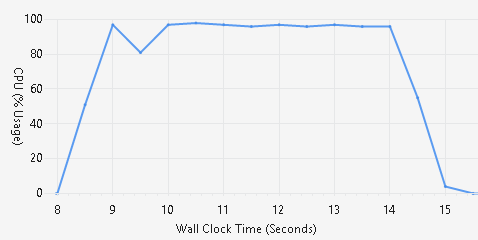
\includegraphics[width=0.9\textwidth]{images/td_hq_impeller_cpu}
	\caption{
		CPU utilization during a run of the tri-dexel algorithm with a grid resolution of 200 along the longest axis, all features enabled, reconstructing the surface of the impeller scene.
		Measured using the profiler of Visual Studio 2013.
	}
	\label{fig:td_hq_impeller_cpu}
\end{figure}
%
The extraction starts by performing a raycast on the VML's data model.
It takes some time in the beginning until the CPU reaches full utilization.
The profiler mostly highlights memory intensive operations during this time, such as pulling the triangles from RAM and allocations.
After 1 - 1.5 seconds, the raycast has finished and the construction of the tri-dexel grid begins.
Again, this process requires a lot of memory allocations, which are serialized by the operating system, causing the utilization to drop slightly.
This drop includes the aggregation of data to form isolated cells, which is memory intensive as well.

Processing cells starts right away after the first cells are available.
At this point the CPU again reaches maximum utilization for almost the complete extraction, as the granularity of the parallelization is quite fine, \ie lots of cells are available to saturate all cores.
However, as fully occupied and non-occupied cells do not need any processing, only boundary cells contribute to the surface, the intensity of a work item varies.
In the last second, triangulation has been finished for almost all cells.
Most of the work left is freeing allocated resources, which takes quite a while and is again serialized by the operating system, causing the utilization to drop drastically for the last second.

Regarding the allocated memory, in addition to the VML's regular grid holding the impeller scene in \SI{600}{\mebi\byte}, the tri-dexel algorithm requires approximately \SI{425}{\mebi\byte} additional memory, mostly for storing the dexel images, grid point occupancies and grid edges with their segments.
On third of the memory is allocated before the raycast, another third during the raycast and the last third when building the tri-dexel grid.
While cells are processed, cell data is aggregated, regularized, triangulated and immediately freed again.
Therefore, the memory consumption remains almost constant during the further execution after the grid construction.

Figure \ref{fig:di_results} contains renderings of the resulting triangle meshes.
%
\begin{figure}
	\centering
	\begin{subfigure}[b]{0.34\textwidth}
		\centering
		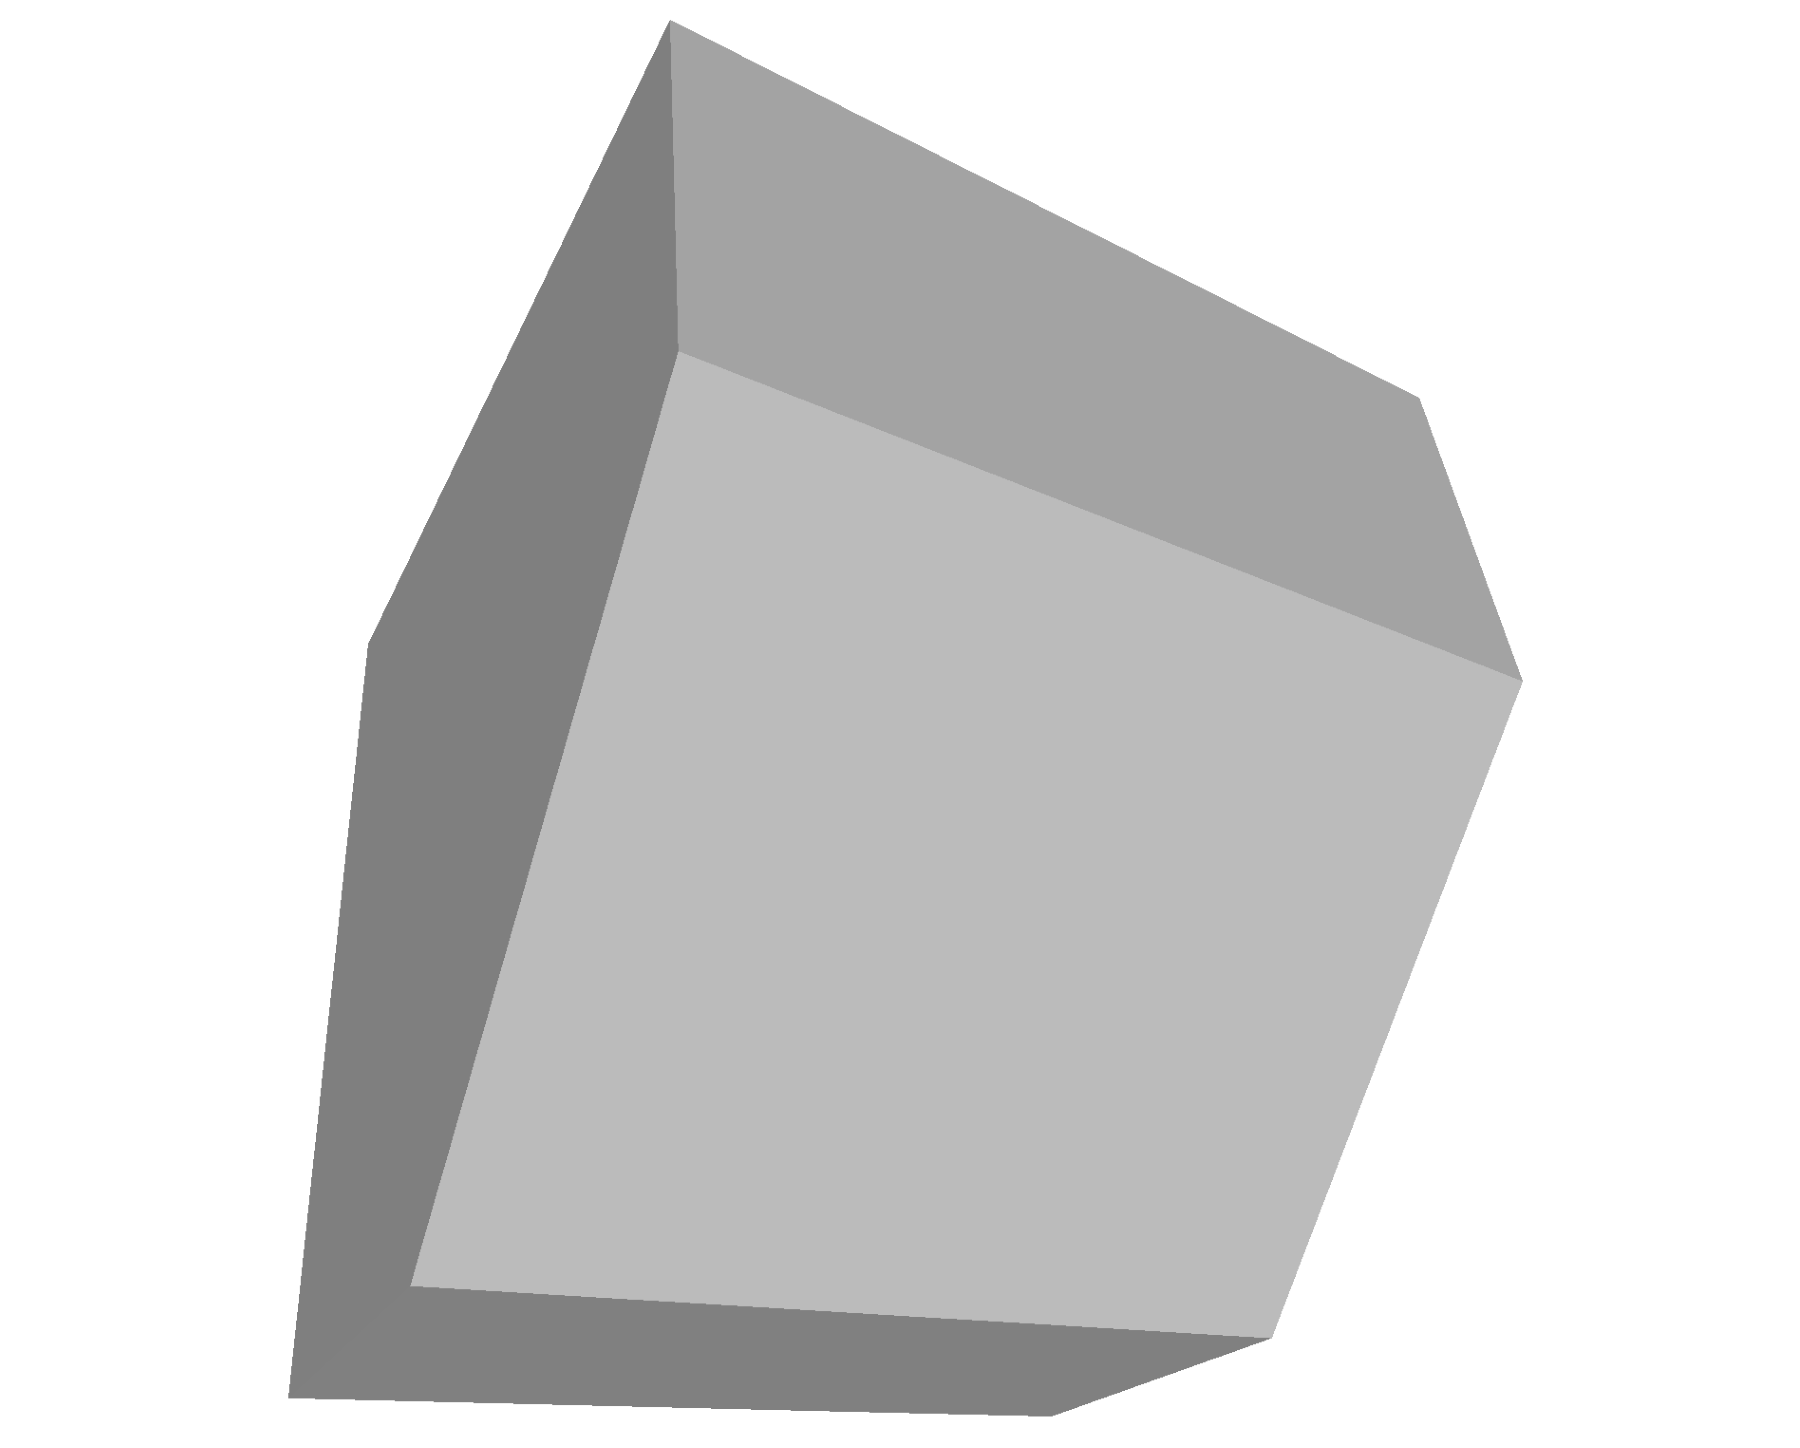
\includegraphics[width=\textwidth]{td_cube2}
		\caption{cube2}
		\label{fig:td_cube2}
	\end{subfigure}
	\hspace{1cm}
	\begin{subfigure}[b]{0.34\textwidth}
		\centering
		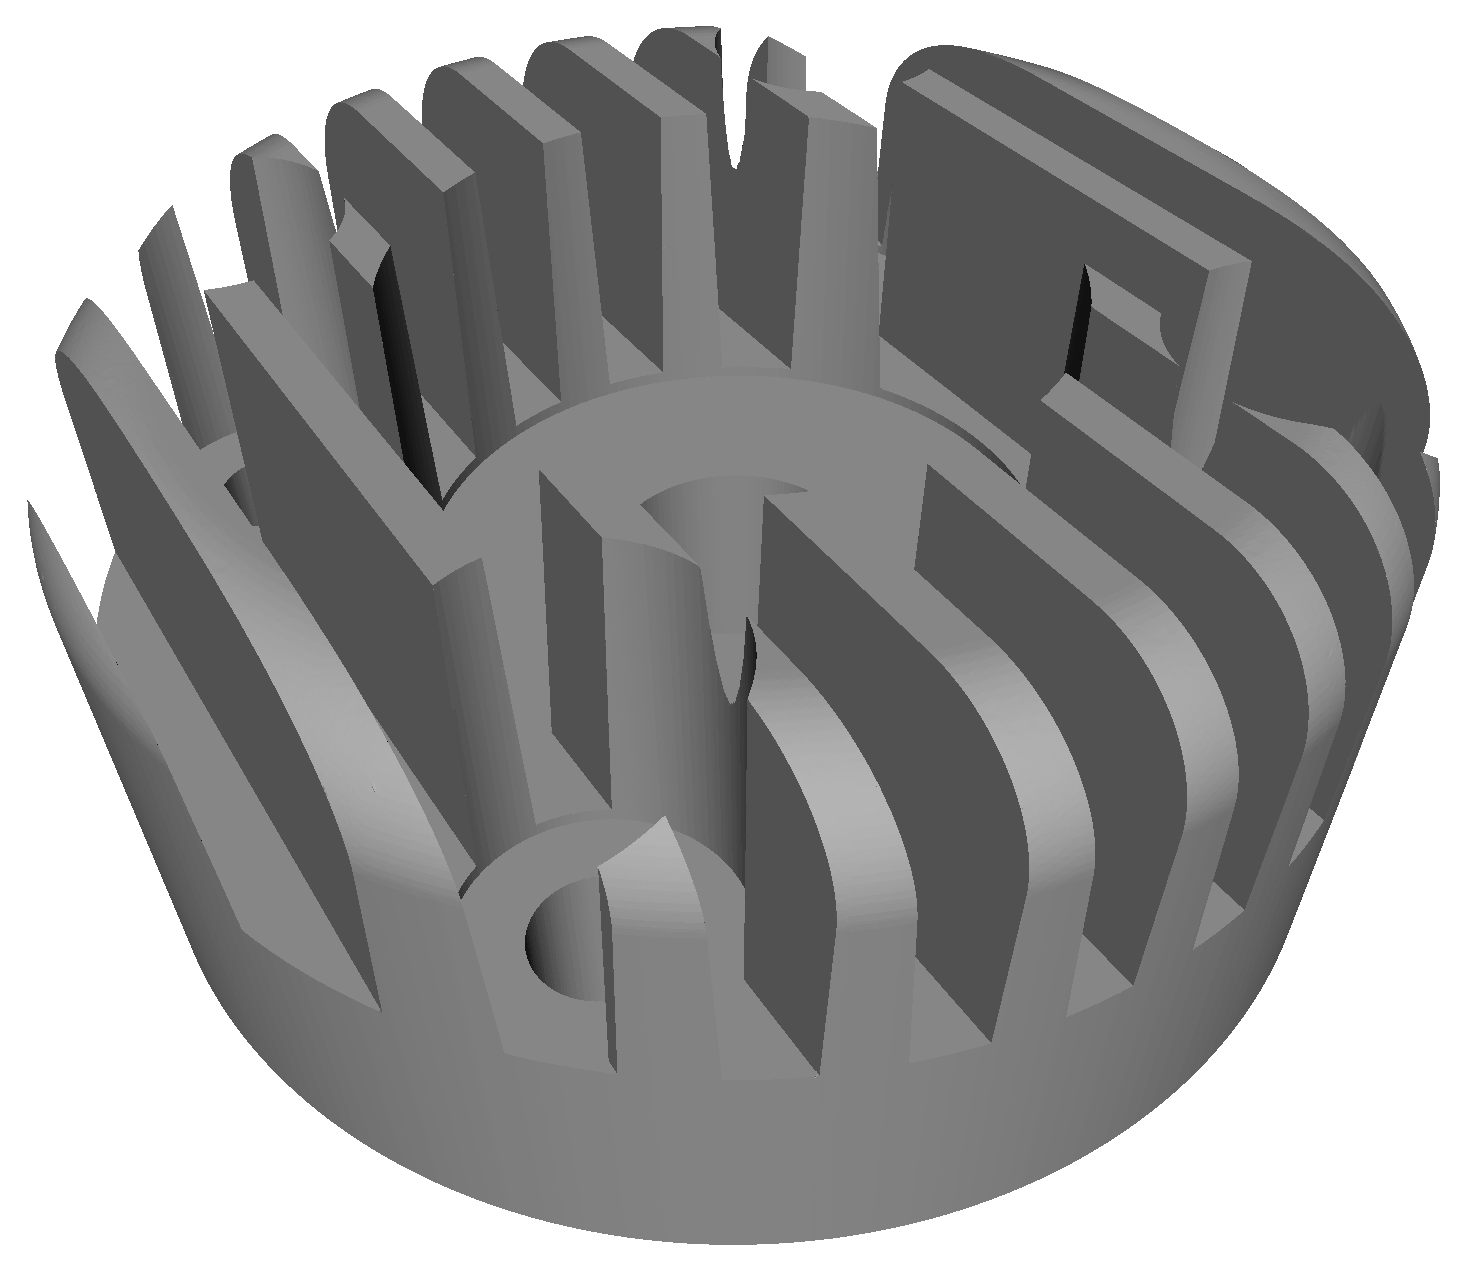
\includegraphics[width=\textwidth]{td_cylinder_head}
		\caption{cylinder\_head}
		\label{fig:td_cylinder_head}
	\end{subfigure}
	\begin{subfigure}[b]{0.34\textwidth}
		\centering
		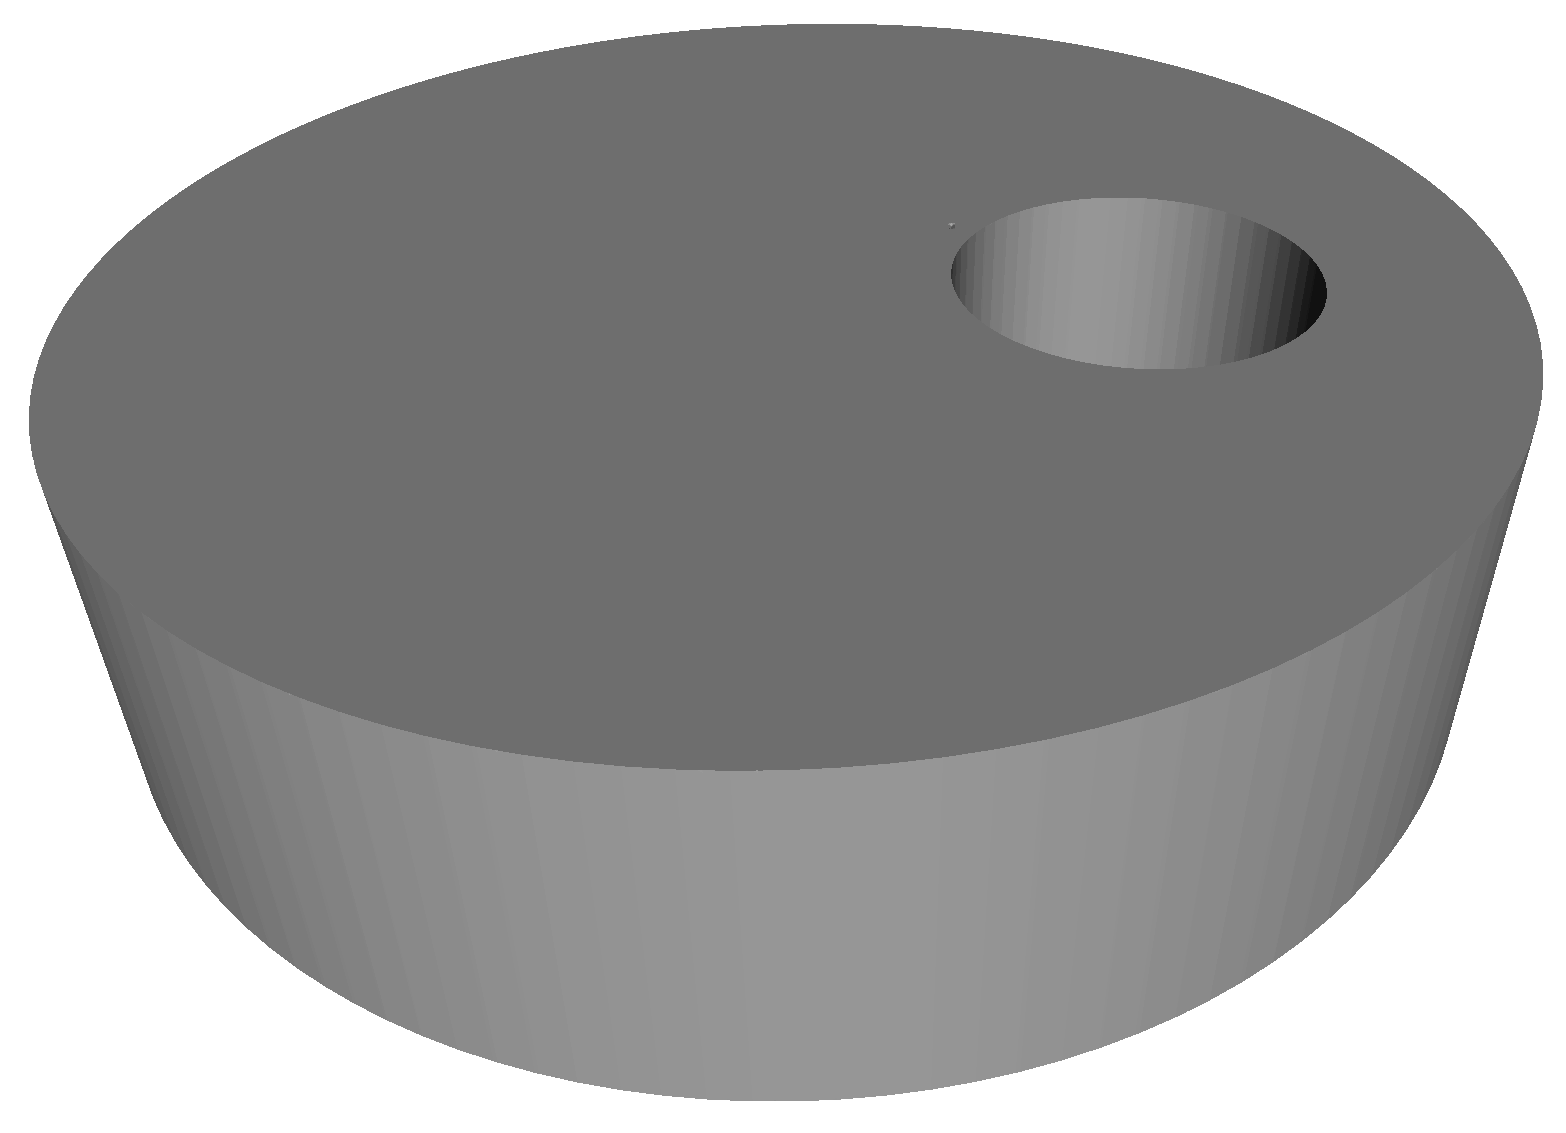
\includegraphics[width=\textwidth]{td_cylinders}
		\caption{cylinders}
		\label{fig:td_cylinders}
	\end{subfigure}
	\hspace{1cm}
	\begin{subfigure}[b]{0.34\textwidth}
		\centering
		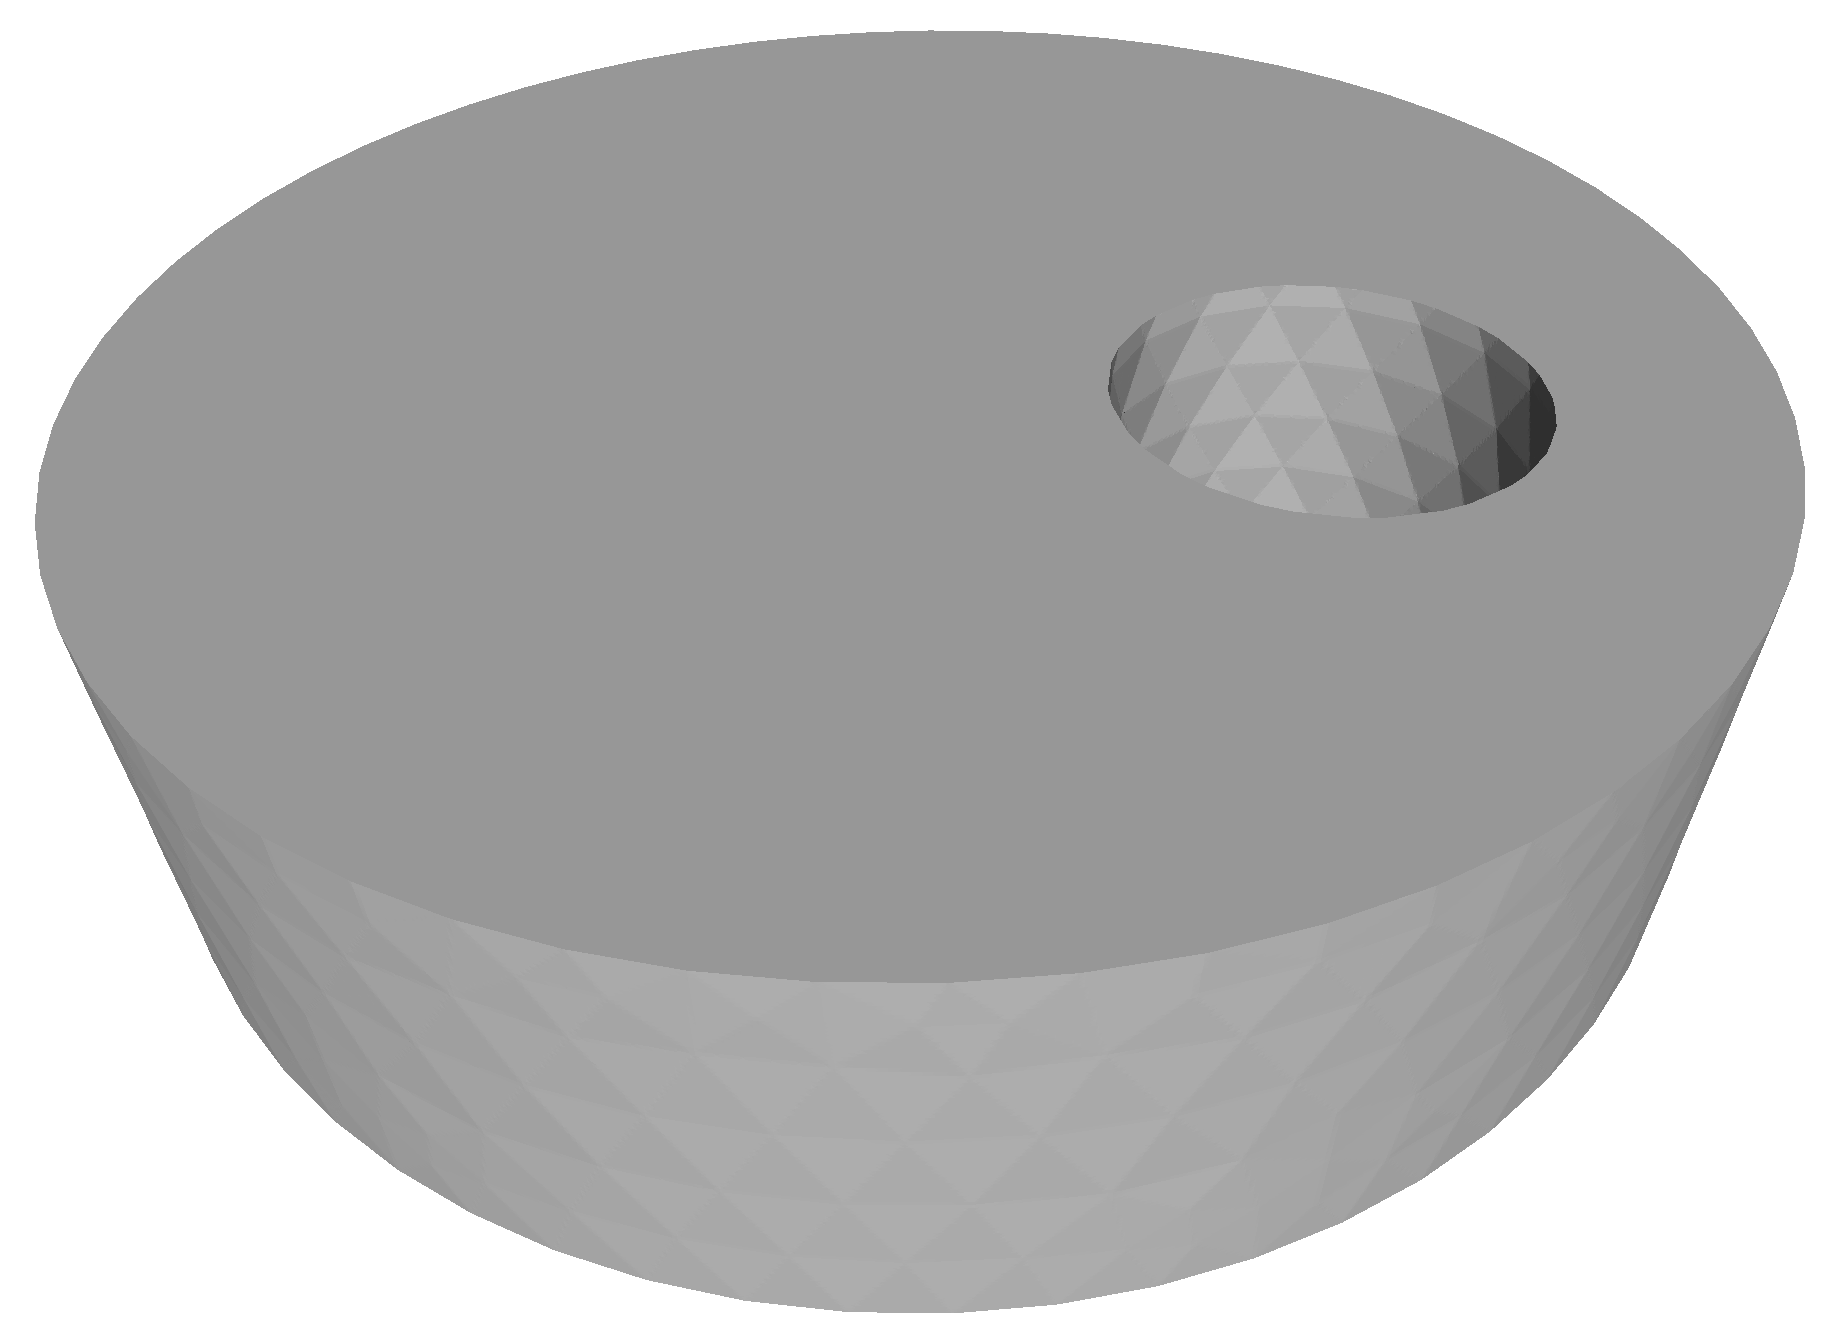
\includegraphics[width=\textwidth]{td_cylinders_d}
		\caption{cylinders\_d}
		\label{fig:td_cylinders_delaunay}
	\end{subfigure}
	\begin{subfigure}[b]{0.34\textwidth}
		\centering
		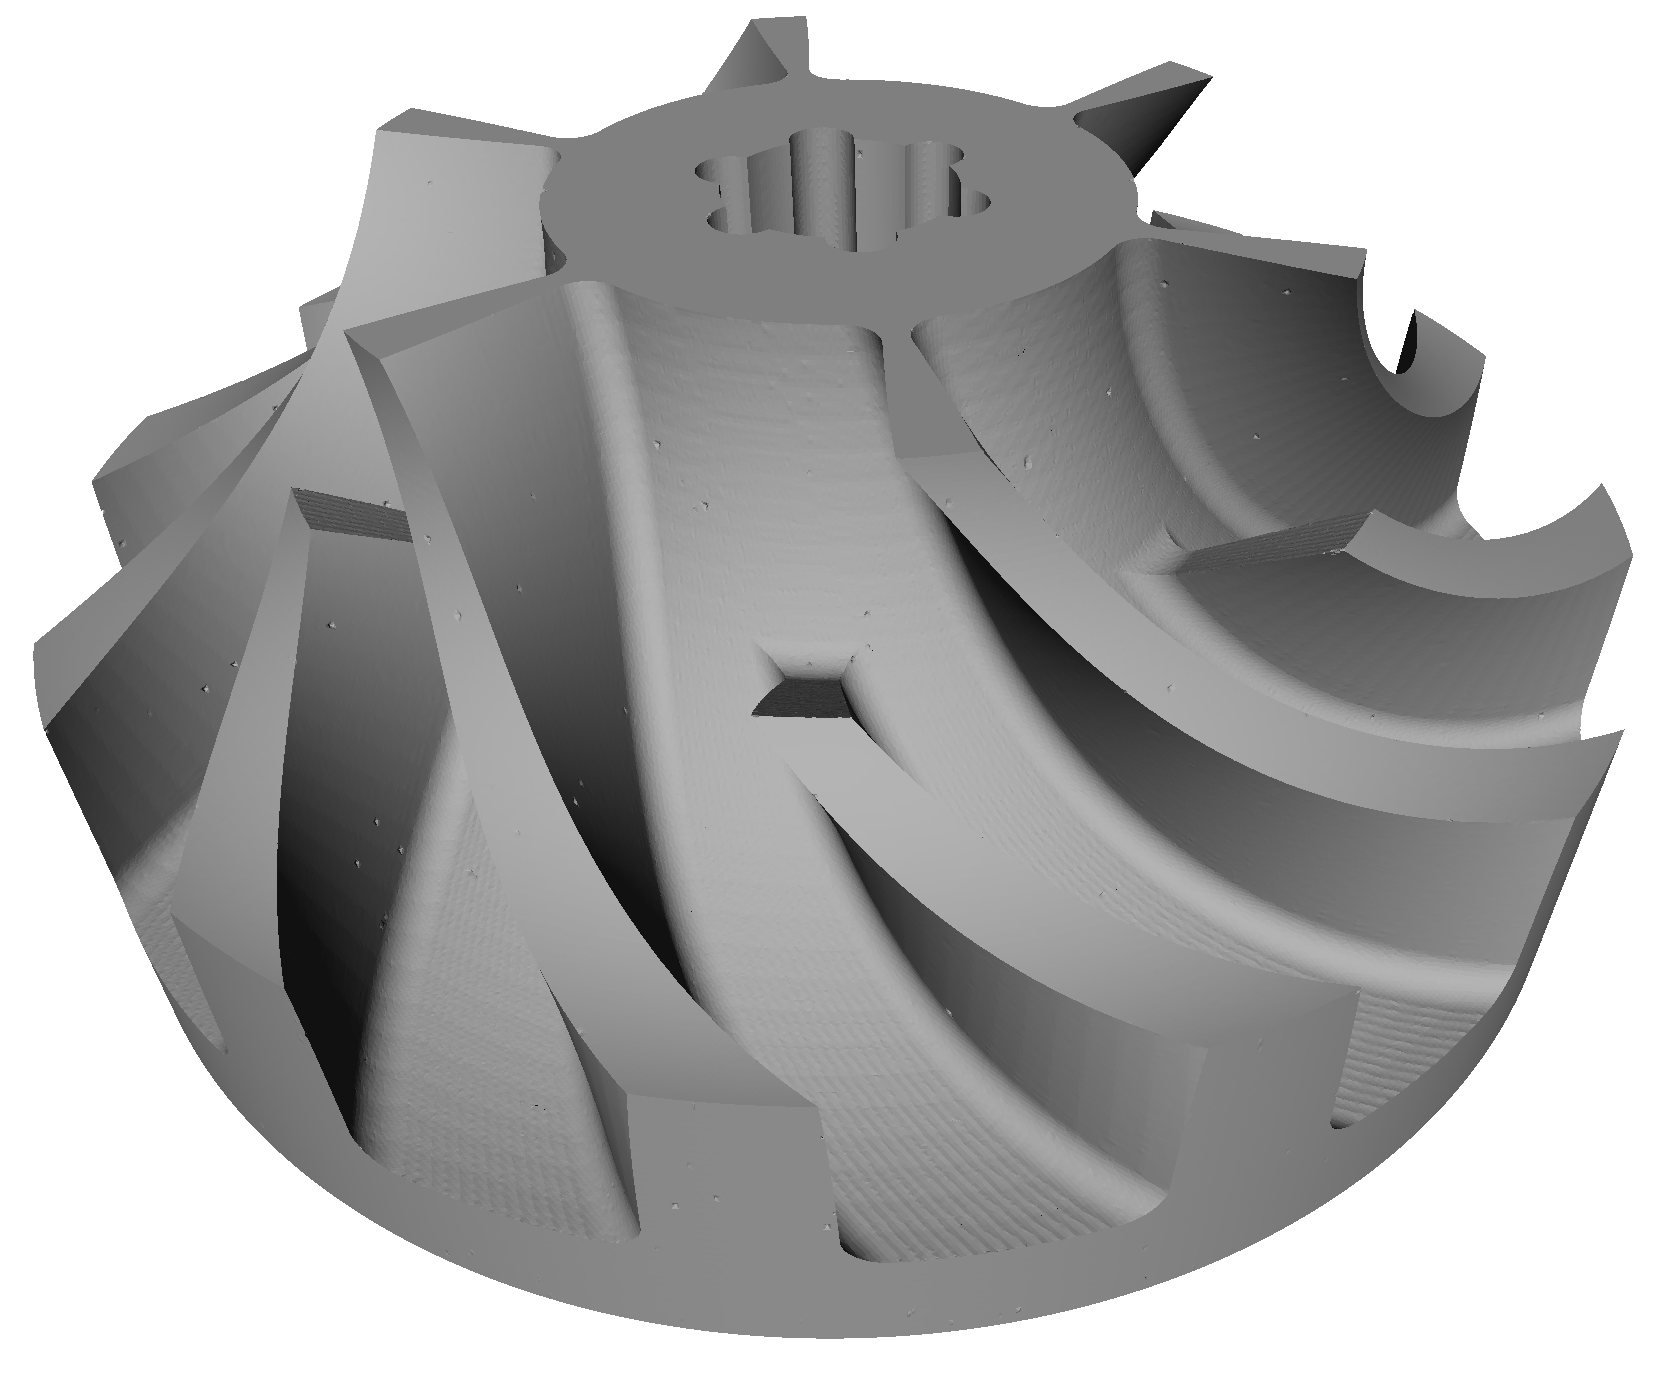
\includegraphics[width=\textwidth]{td_hq_impeller}
		\caption{impeller}
		\label{fig:td_hq_impeller}
	\end{subfigure}
	\hspace{1cm}
	\begin{subfigure}[b]{0.34\textwidth}
		\centering
		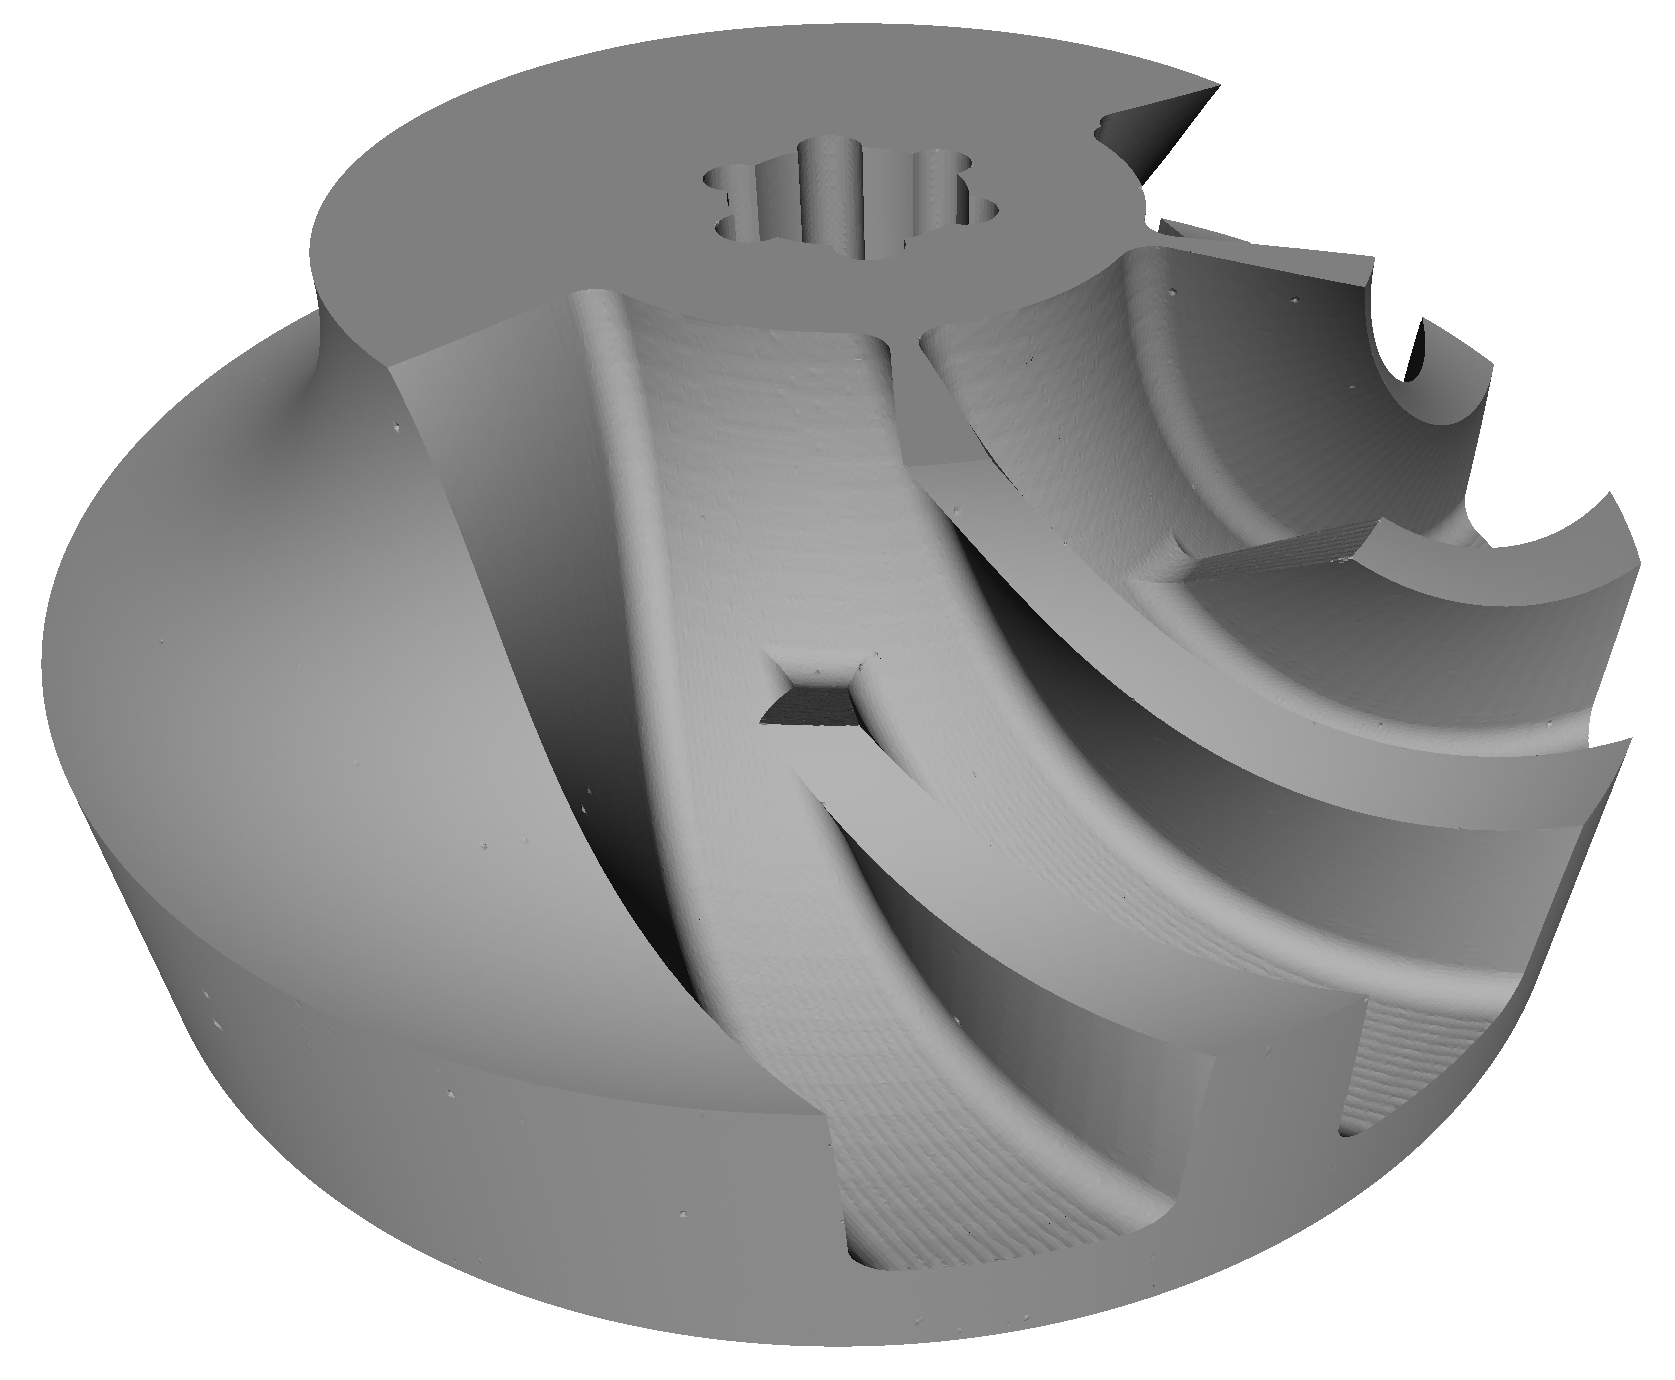
\includegraphics[width=\textwidth]{td_hq_impeller_2}
		\caption{impeller\_2}
		\label{fig:td_hq_impeller_2}
	\end{subfigure}
	\begin{subfigure}[b]{0.33\textwidth}
		\centering
		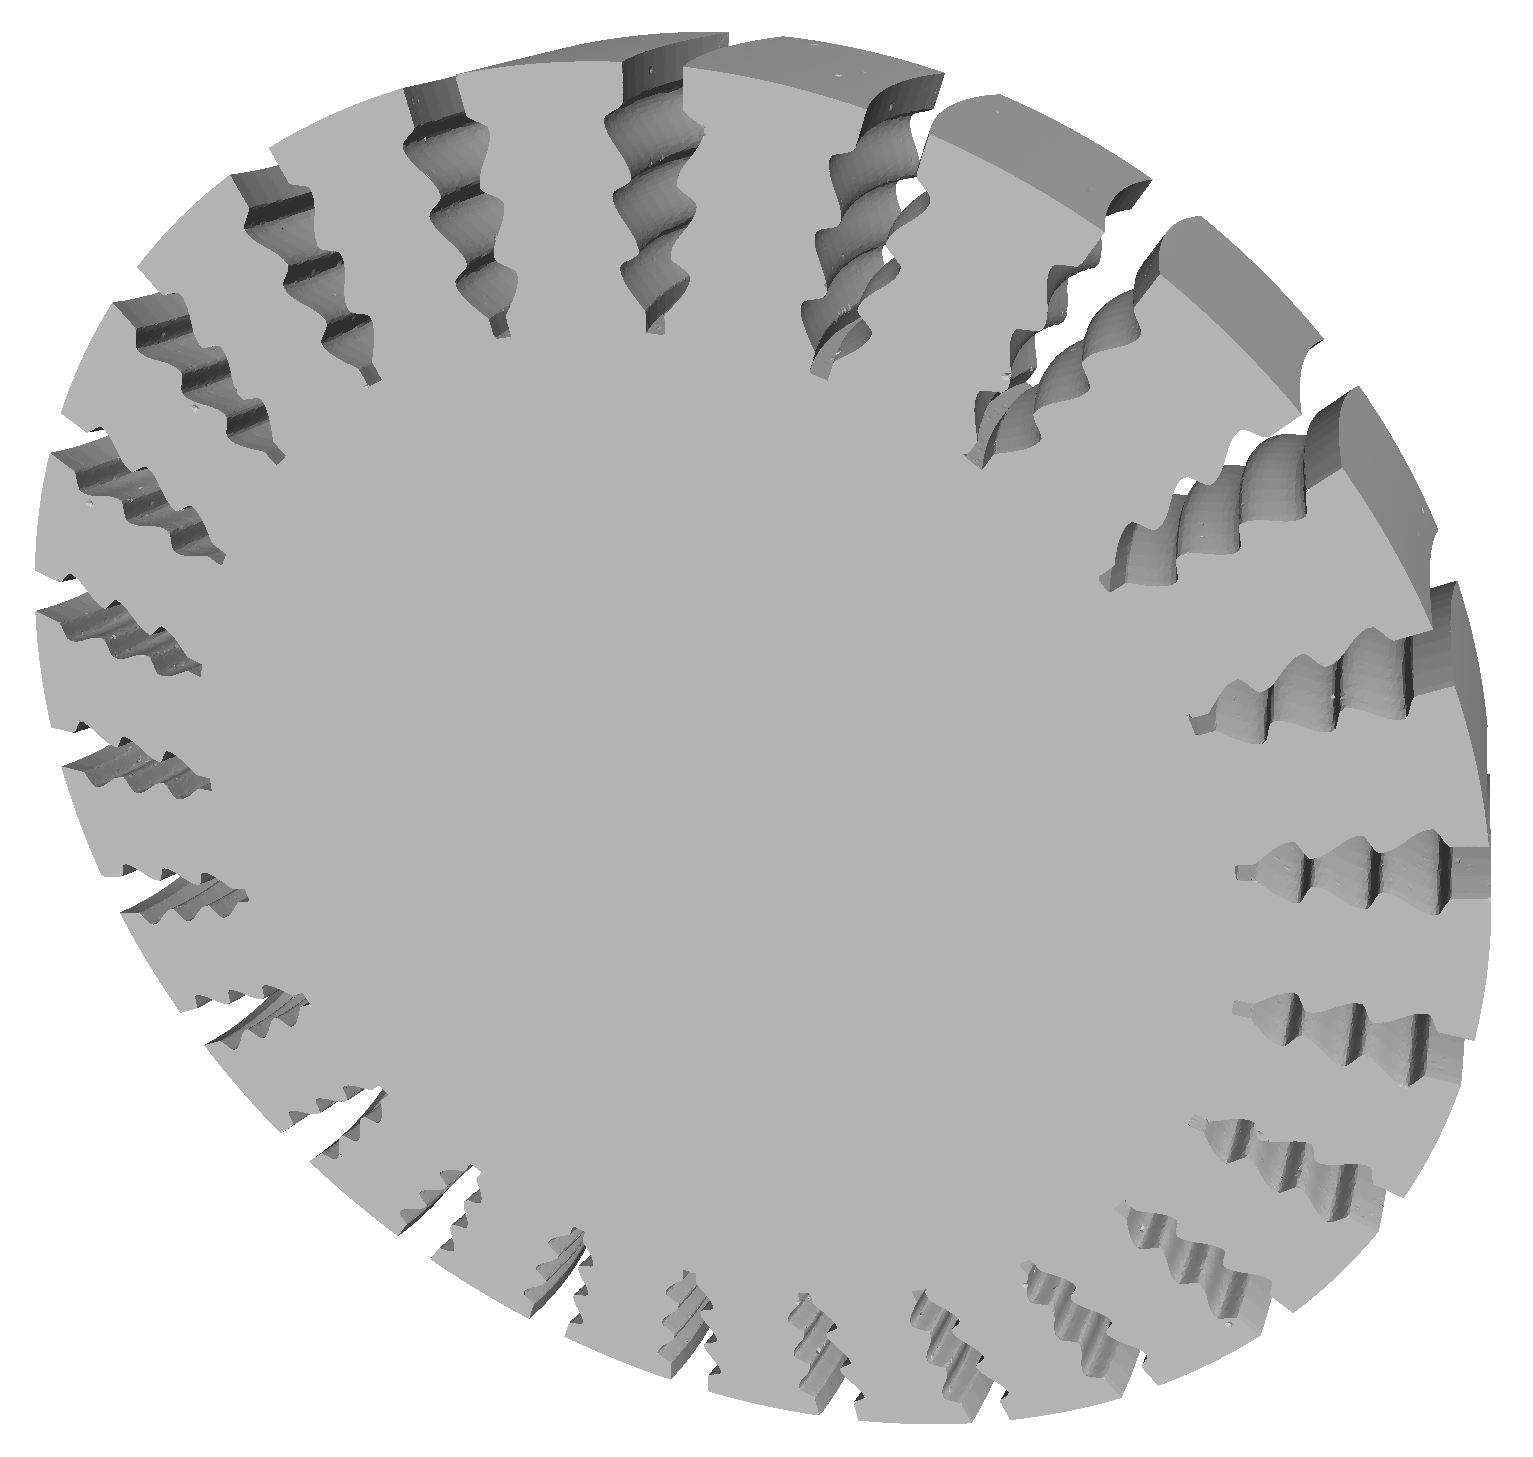
\includegraphics[width=\textwidth]{td_turbine}
		\caption{turbine}
		\label{fig:td_turbine}
	\end{subfigure}
	\caption{
		Renderings of the result meshes using MeshLab after applying the tri-dexel reconstruction approach with a resolution of 400 on the selected test scenes in table \ref{tbl:test_scenes}.
	}
	\label{fig:td_results}
\end{figure}
%
The cube2 scene has been extracted flawlessly.
All features, \ie edges and corners, of the cube have been perfectly reconstructed.
The only flaw is the high number of triangles outputted, \cf table \ref{tbl:tri_dexel_results}.
However, this number is steered by the dexel grid's resolution and may be set very low for this simple scene.
Furthermore, an additional post-processing pass may be used to recombine adjacent triangles facing in the same direction\footnote{Third-party tools may also be used to manually reduce the triangle count, \eg MeshLab's Quadric Edge Collapse Decimation filter.}.

Both of the cylinders scenes deliver great results as well.
They show perfect edges at the stock as well as at the intersection with the smaller cylindrical swept volume.
However, the cylinders scene, on the top and bottom side, contains a small notch beside the hole drilled out.
This small error is the result of a numeric miscalculation in the raycaster, due to the thin triangles, which could not correctly identify the surface entry and exit for two incident rays.
Therefore, two dexels are completely empty at this location.
This case is handled by regularization rule 3, which creates small segments at the grid's occupied points where the two dexels are empty.
The cylinders\_d scene does not contain any notches or other errors.
Concerning the feature reconstruction capabilities, the algorithm also managed to recover the shape of the original triangulation, which is clearly visible at the side of the stock and at the drilled hole.

Furthermore, the impeller scenes have been extracted very well too.
Figure \ref{fig:td_hq_impeller_details} shows two detailed renderings.
%
\begin{figure}
	\centering
	\begin{subfigure}[b]{0.49\textwidth}
		\centering
		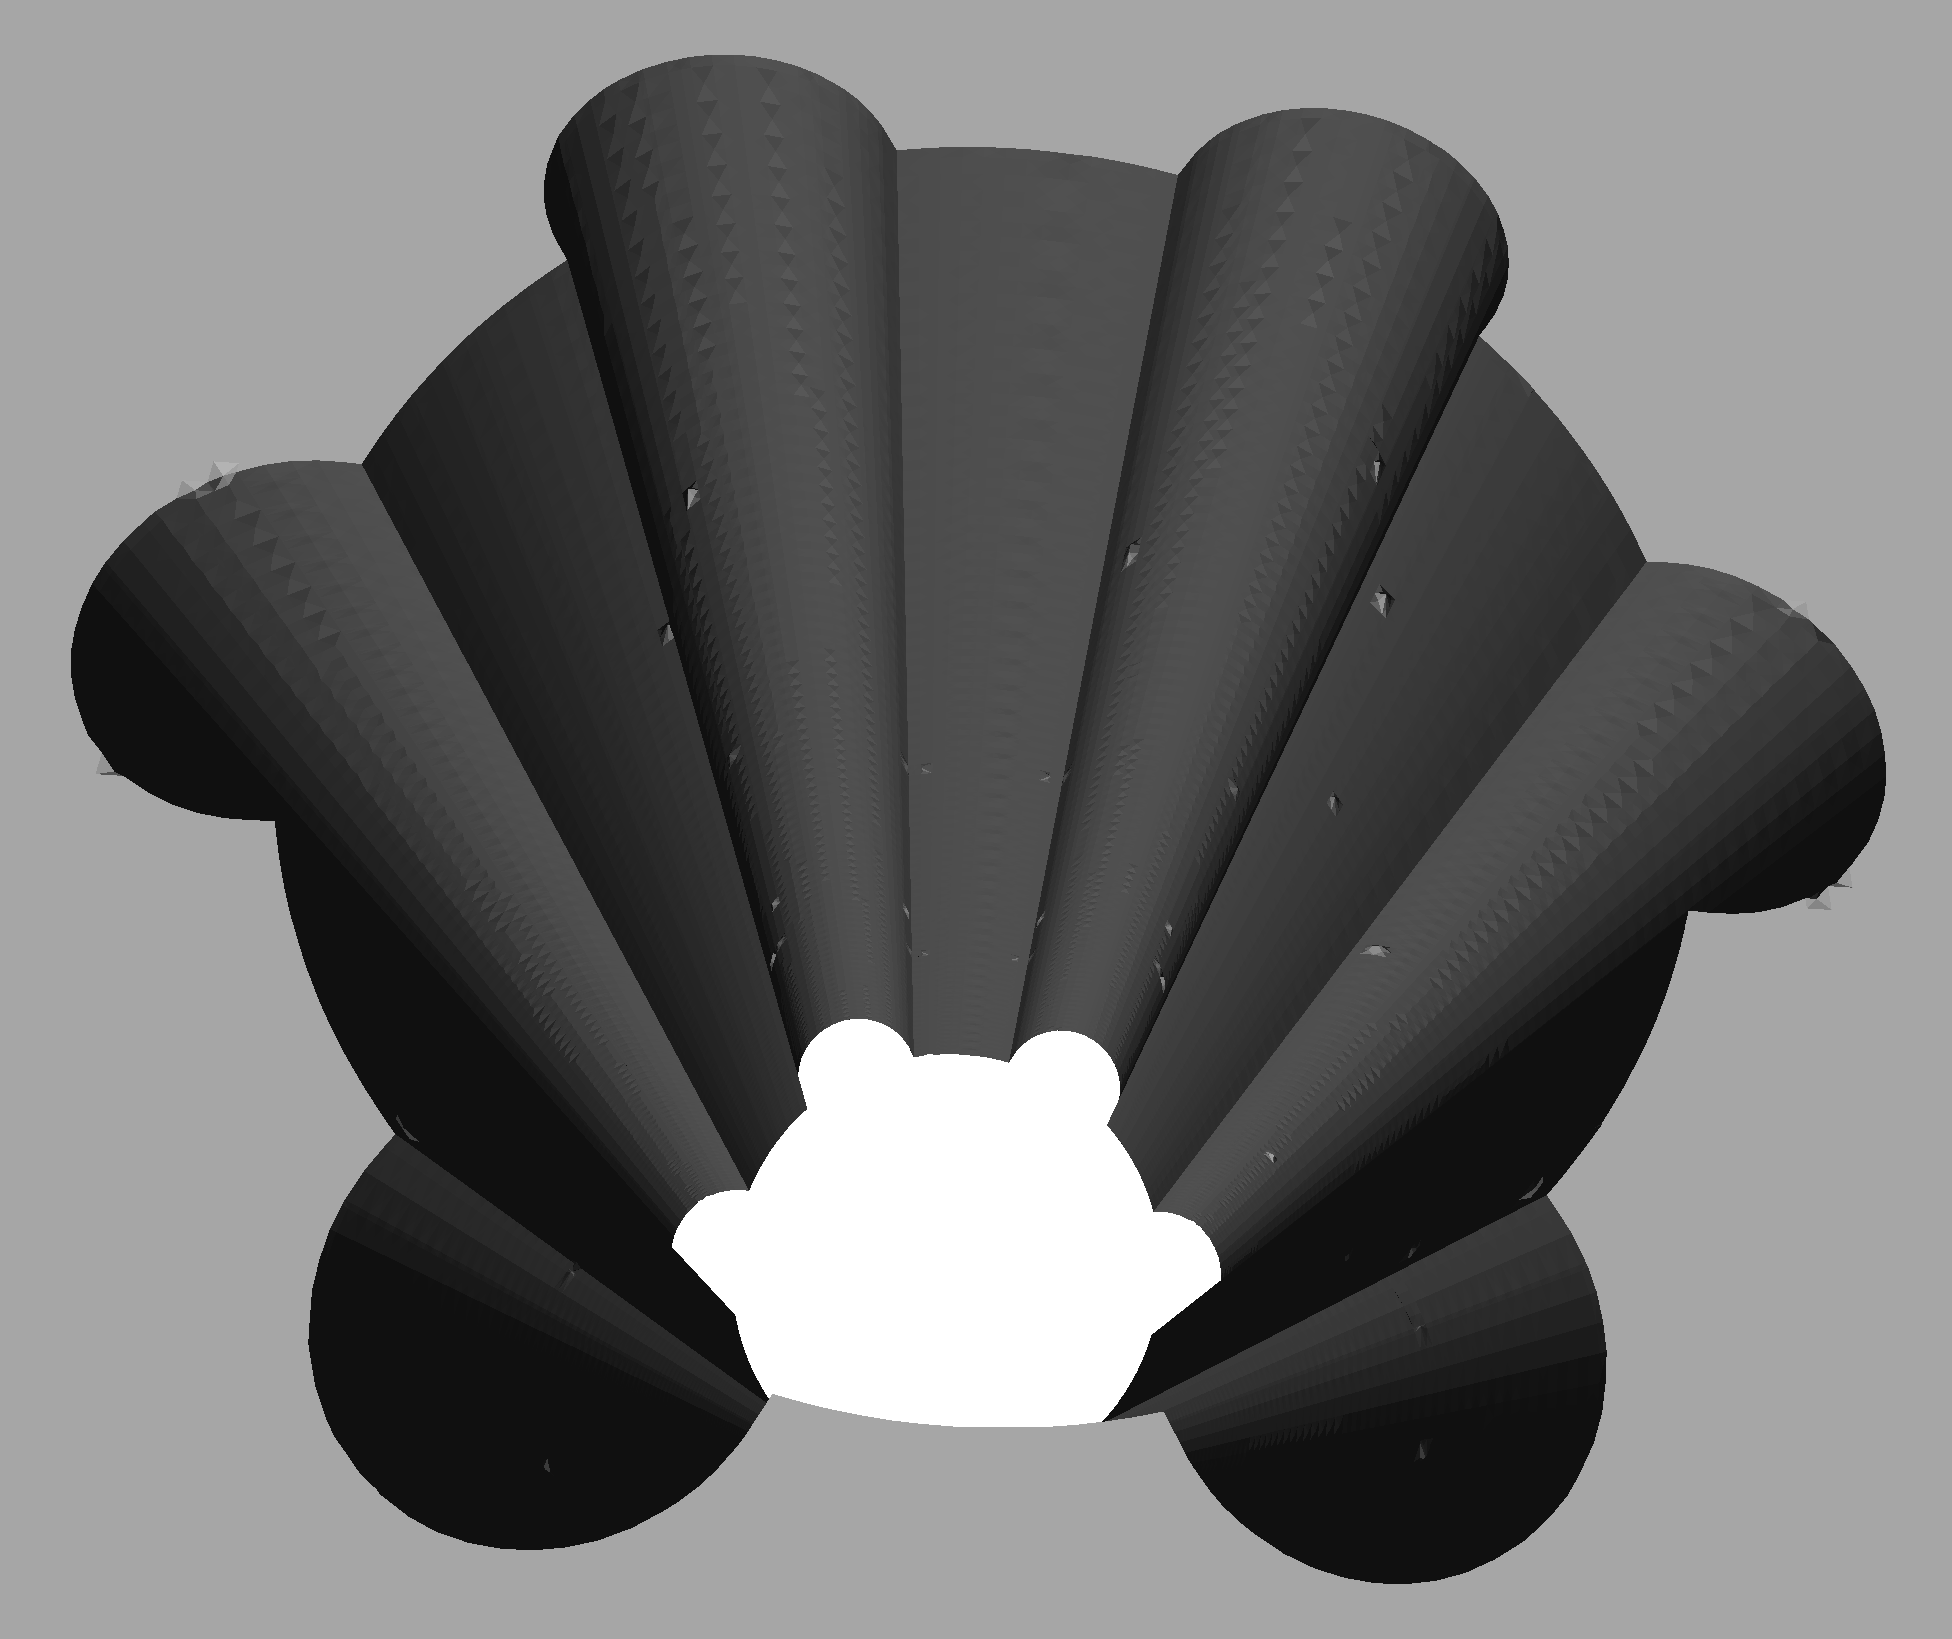
\includegraphics[width=\textwidth]{td_hq_impeller_drillings}
		\caption{impeller drillings}
		\label{fig:td_hq_impeller_drillings}
	\end{subfigure}
	\begin{subfigure}[b]{0.49\textwidth}
		\centering
		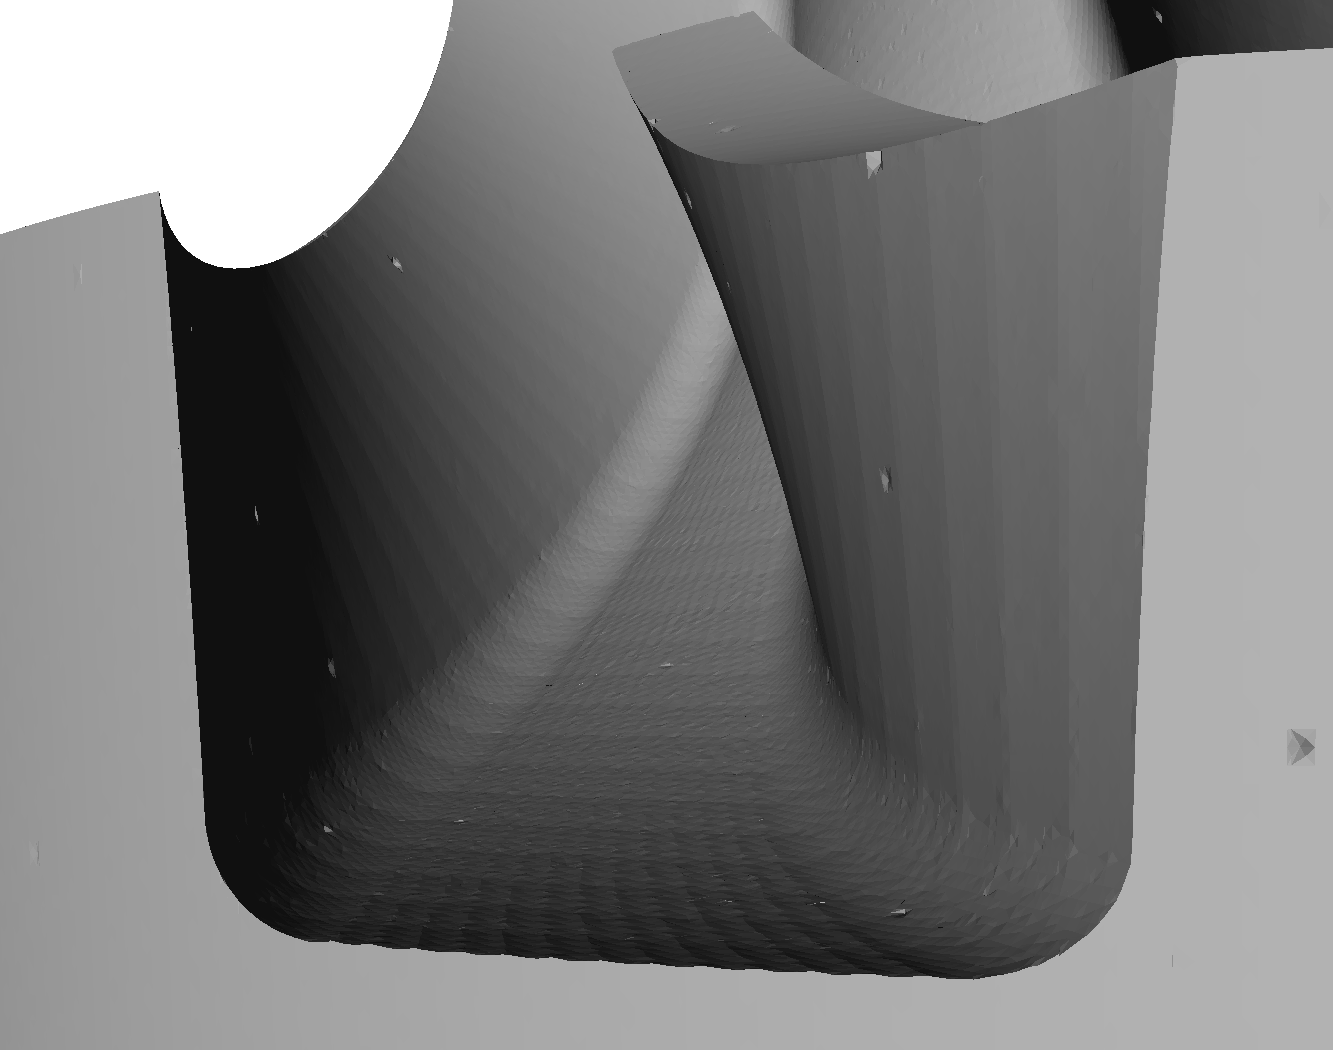
\includegraphics[width=\textwidth]{td_hq_impeller_blades}
		\caption{impeller blades}
		\label{fig:td_hq_impeller_blades}
	\end{subfigure}
	\caption{
		Details of the impeller scene rendered using MeshLab.
		The meshes have been extracted using the tri-dexel approach with a resolution of 400.
	}
	\label{fig:td_hq_impeller_details}
\end{figure}
%
The drillings in the middle resemble the cylindrical swept volumes perfectly, \cf figure \ref{fig:td_hq_impeller_drillings}.
The impeller's blades have sharp edges and, between them, even the rills of the single swept volumes are slightly visible, \cf figure \ref{fig:td_hq_impeller_blades}.
Nonetheless, similarly to the cylinders scene, several numeric issues occurred during the dexel image creation by the raycaster, resulting in numerous notches at the surface.

Finally, the turbine scene looks good as well.
However, as the turbine's grooves contain mostly concave features, a sufficient resolution is required to capture the scene's small peculiarities.
Figure \ref{fig:td_grooves} shows renderings of a detailed view on one of the turbine's grooves in different resolutions.
%
\begin{figure}
	\centering
	\begin{subfigure}[b]{0.24\textwidth}
		\centering
		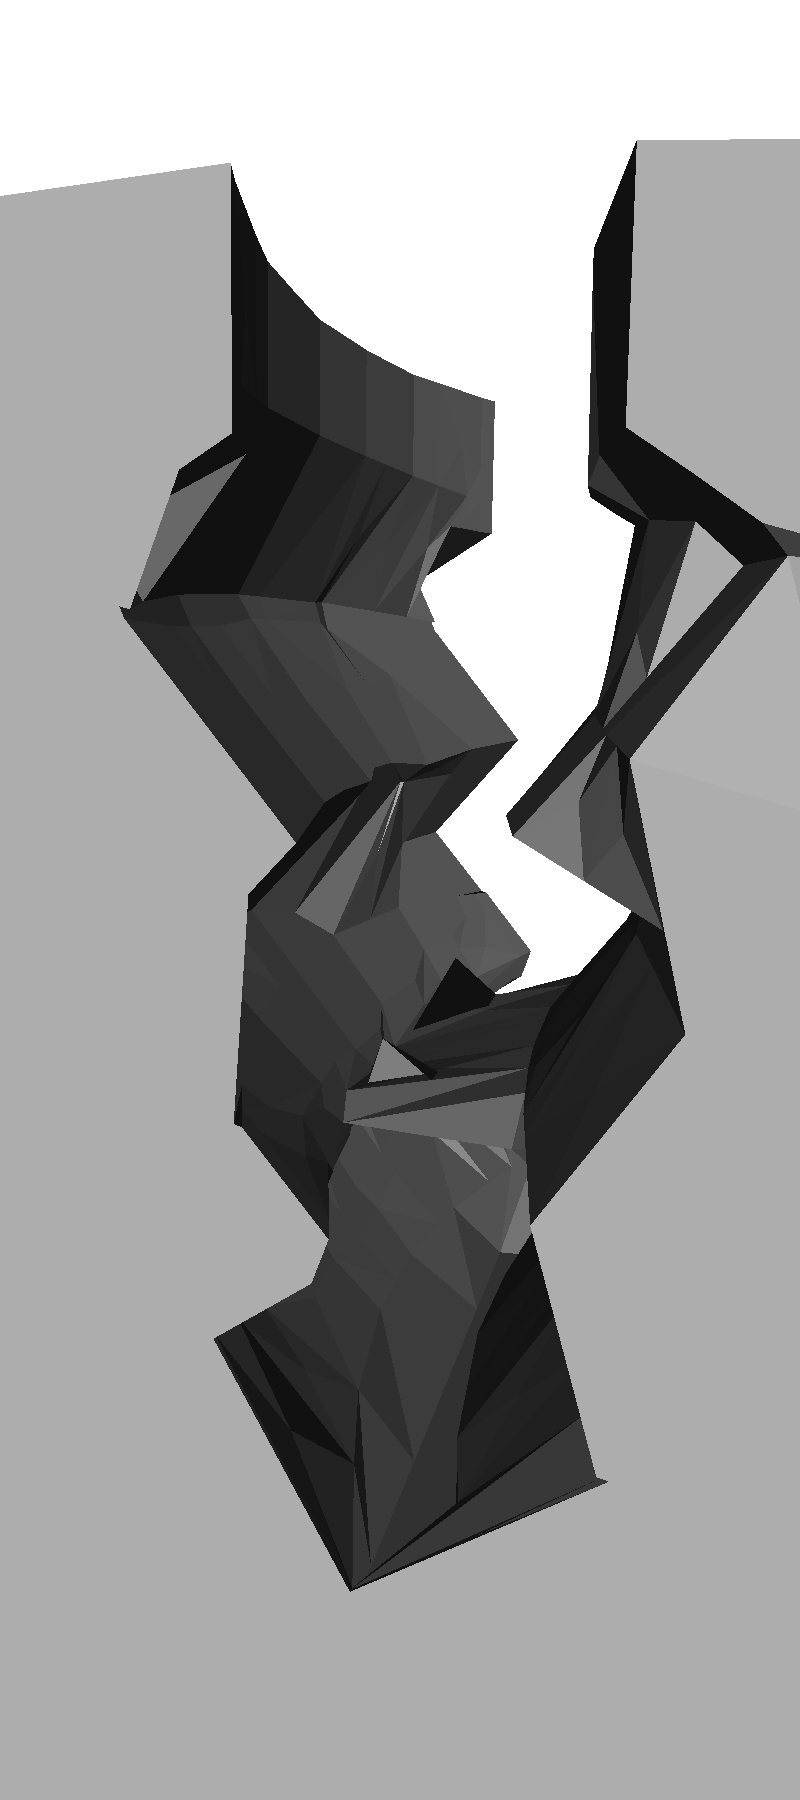
\includegraphics[width=\textwidth]{td_turbine_groove_50}
		\caption{50}
		\label{fig:td_turbine_groove_50}
	\end{subfigure}
	\begin{subfigure}[b]{0.24\textwidth}
		\centering
		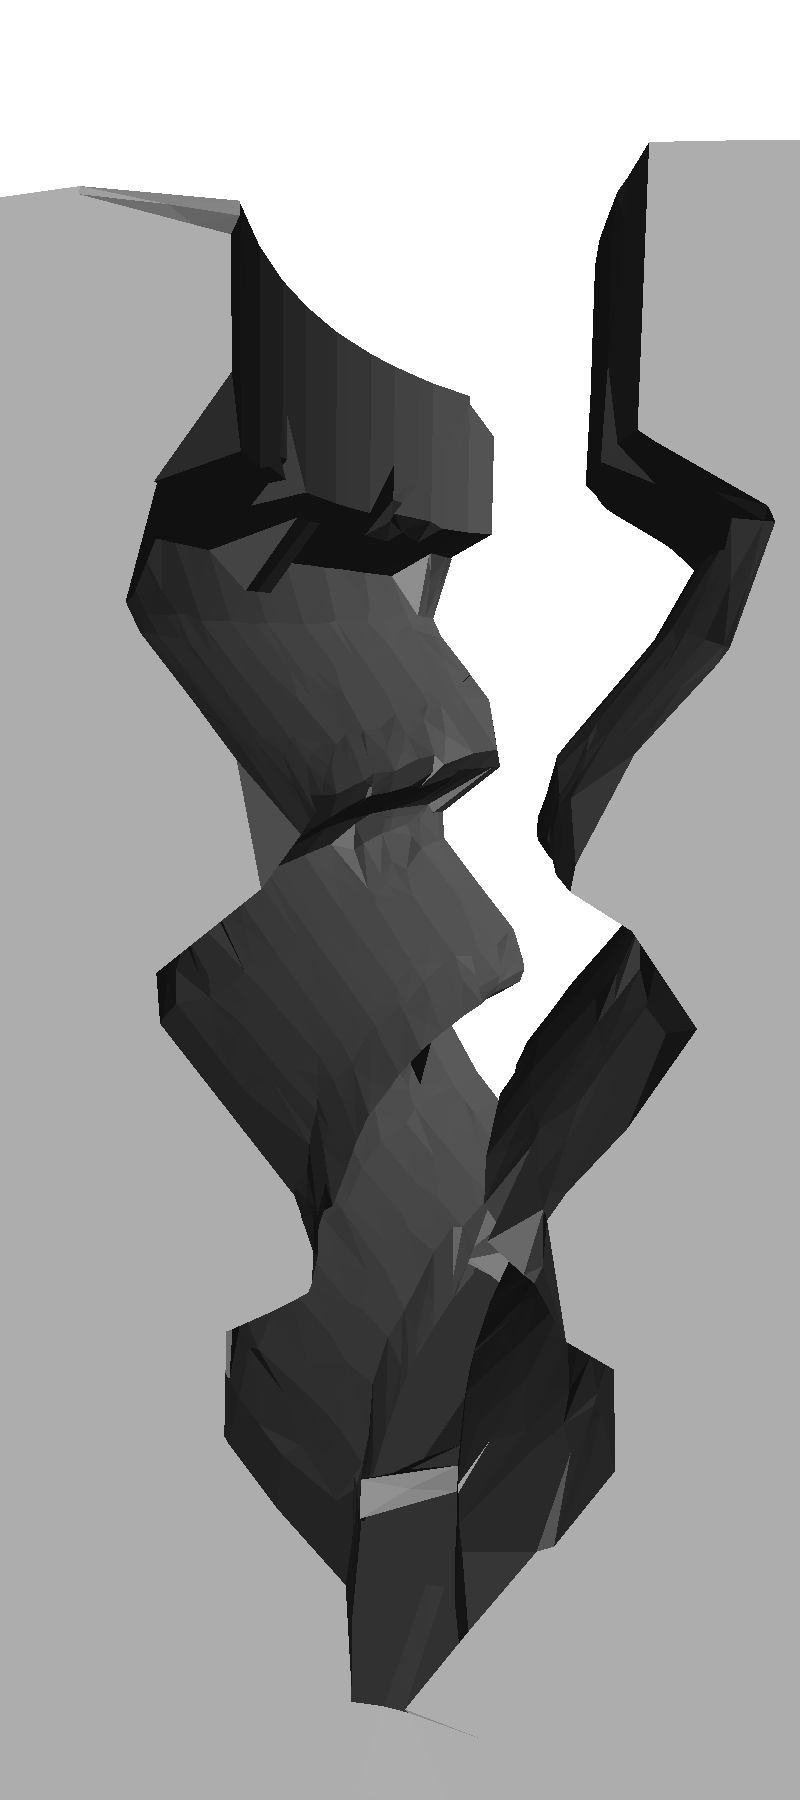
\includegraphics[width=\textwidth]{td_turbine_groove_100}
		\caption{100}
		\label{fig:td_turbine_groove_100}
	\end{subfigure}
	\begin{subfigure}[b]{0.24\textwidth}
		\centering
		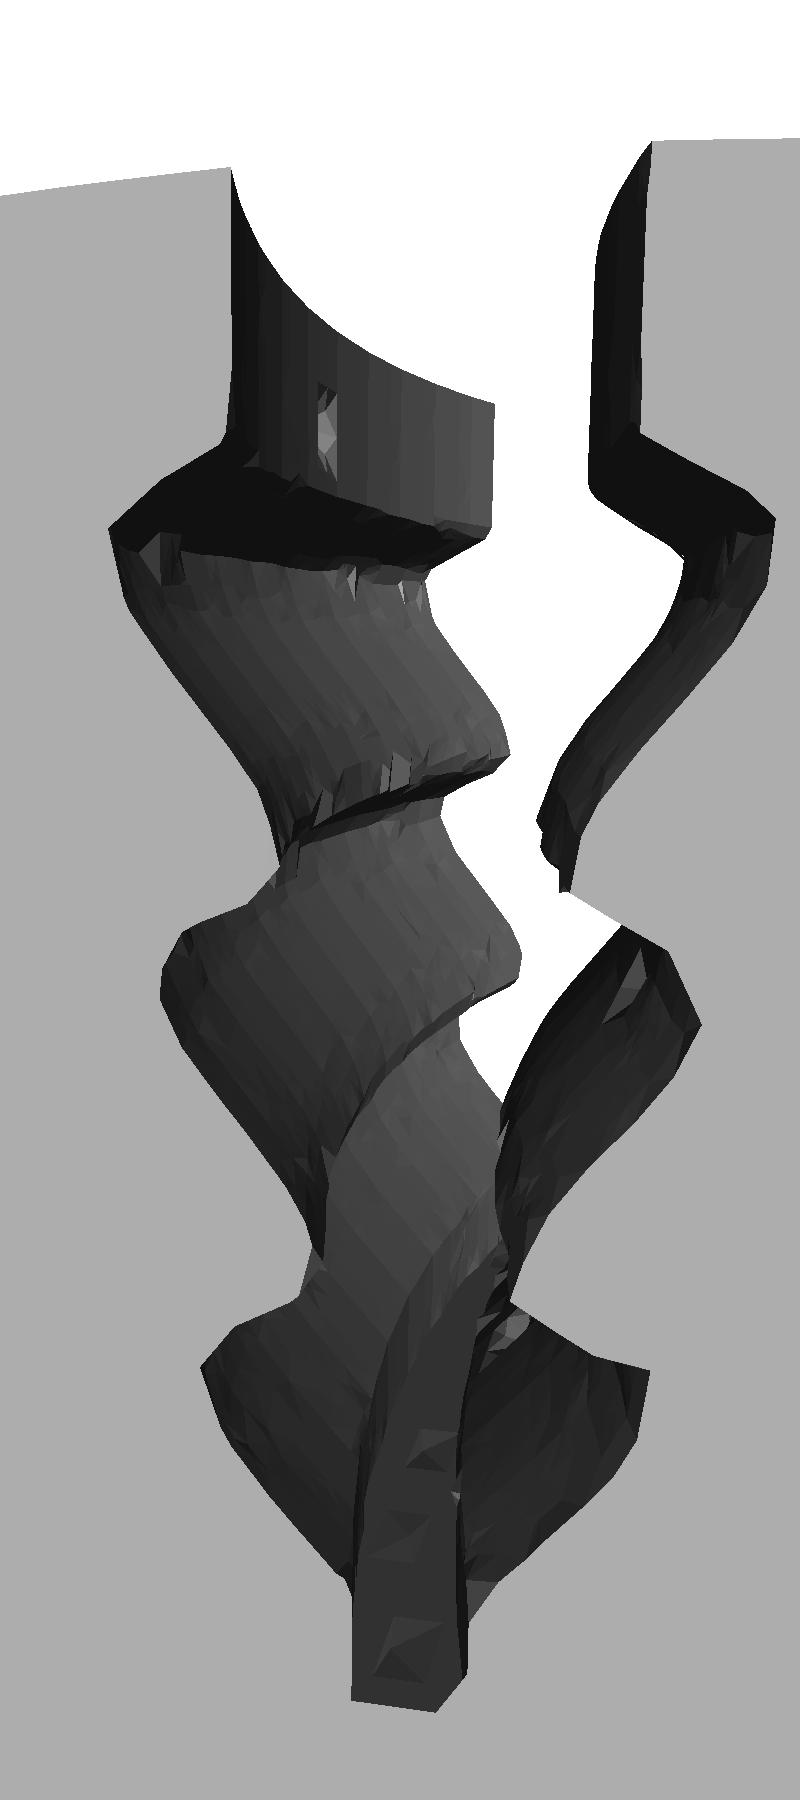
\includegraphics[width=\textwidth]{td_turbine_groove_200}
		\caption{200}
		\label{fig:td_turbine_groove_200}
	\end{subfigure}
	\begin{subfigure}[b]{0.24\textwidth}
		\centering
		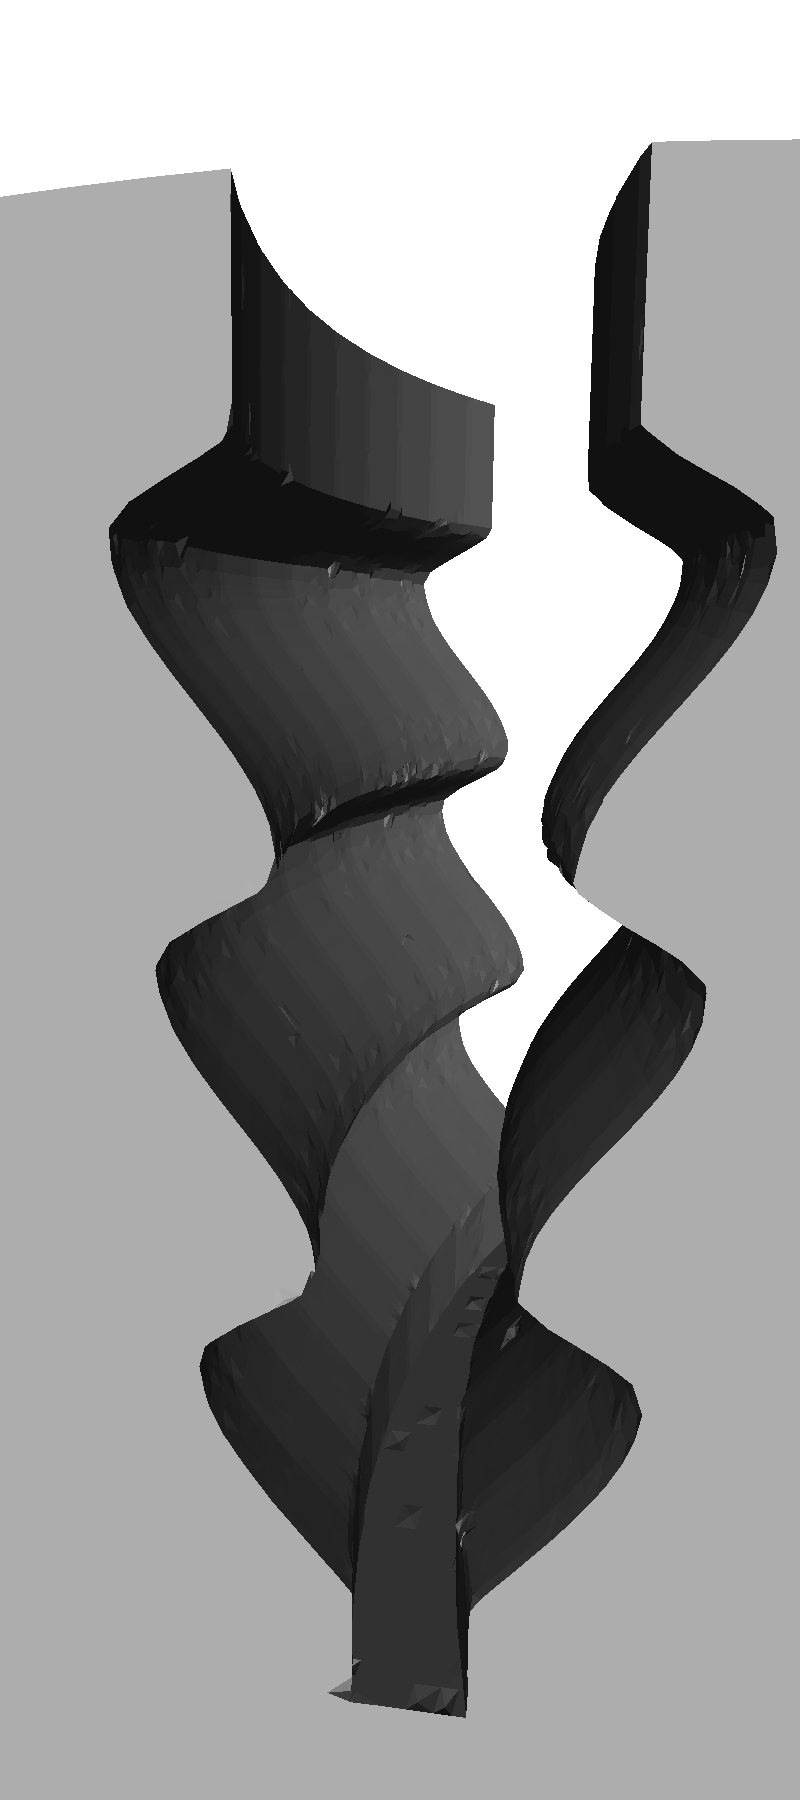
\includegraphics[width=\textwidth]{td_turbine_groove_400}
		\caption{400}
		\label{fig:td_turbine_groove_400}
	\end{subfigure}
	\caption{
		Detailed renderings with the same perspective of a groove of the turbine scene using MeshLab.
		The meshes were created using the tri-dexel reconstruction algorithm with the resolutions 50, 100, 200 and 400.
	}
	\label{fig:td_grooves}
\end{figure}
%
At a resolution of 50, the groove itself is spanned by a bit of geometry.
Doubling the resolution lets the tri-dexel algorithm reconstruct the groove but leaves some geometry left in the wavy sides of the groove.
Increasing the level of detail to a resolution of 200 already retrieves a quite good surface with only a few missing subtleties at the tips of the waves.
These are finally reconstructed using a resolution of 400.
Nonetheless, a few errors still remain due to irregularities on the dexel image caused by misjudgments of the raycaster.

Concluding, all extracted meshes offer great detail.
Especially convex features like sharp corners and edges are retrieved almost perfectly.
Concave features, like the ones of the turbine, seem a bit harder to reconstruct and require an appropriate resolution.

Without using cell slicing, all meshes are manifold, closed and orientable.
Enhancing the tri-dexel approach by slicing irregular cells greatly reduces dropping valuable information during regularization, resulting in far better refined features.
Figure \ref{fig:td_features_and_cell_slicing} shows the difference of the reconstructed mesh when using no refinement/feature reconstruction, when using feature reconstruction and when using feature reconstruction and cell slicing.
%
\begin{figure}
	\centering
	\begin{subfigure}[b]{0.67\textwidth}
		\centering
		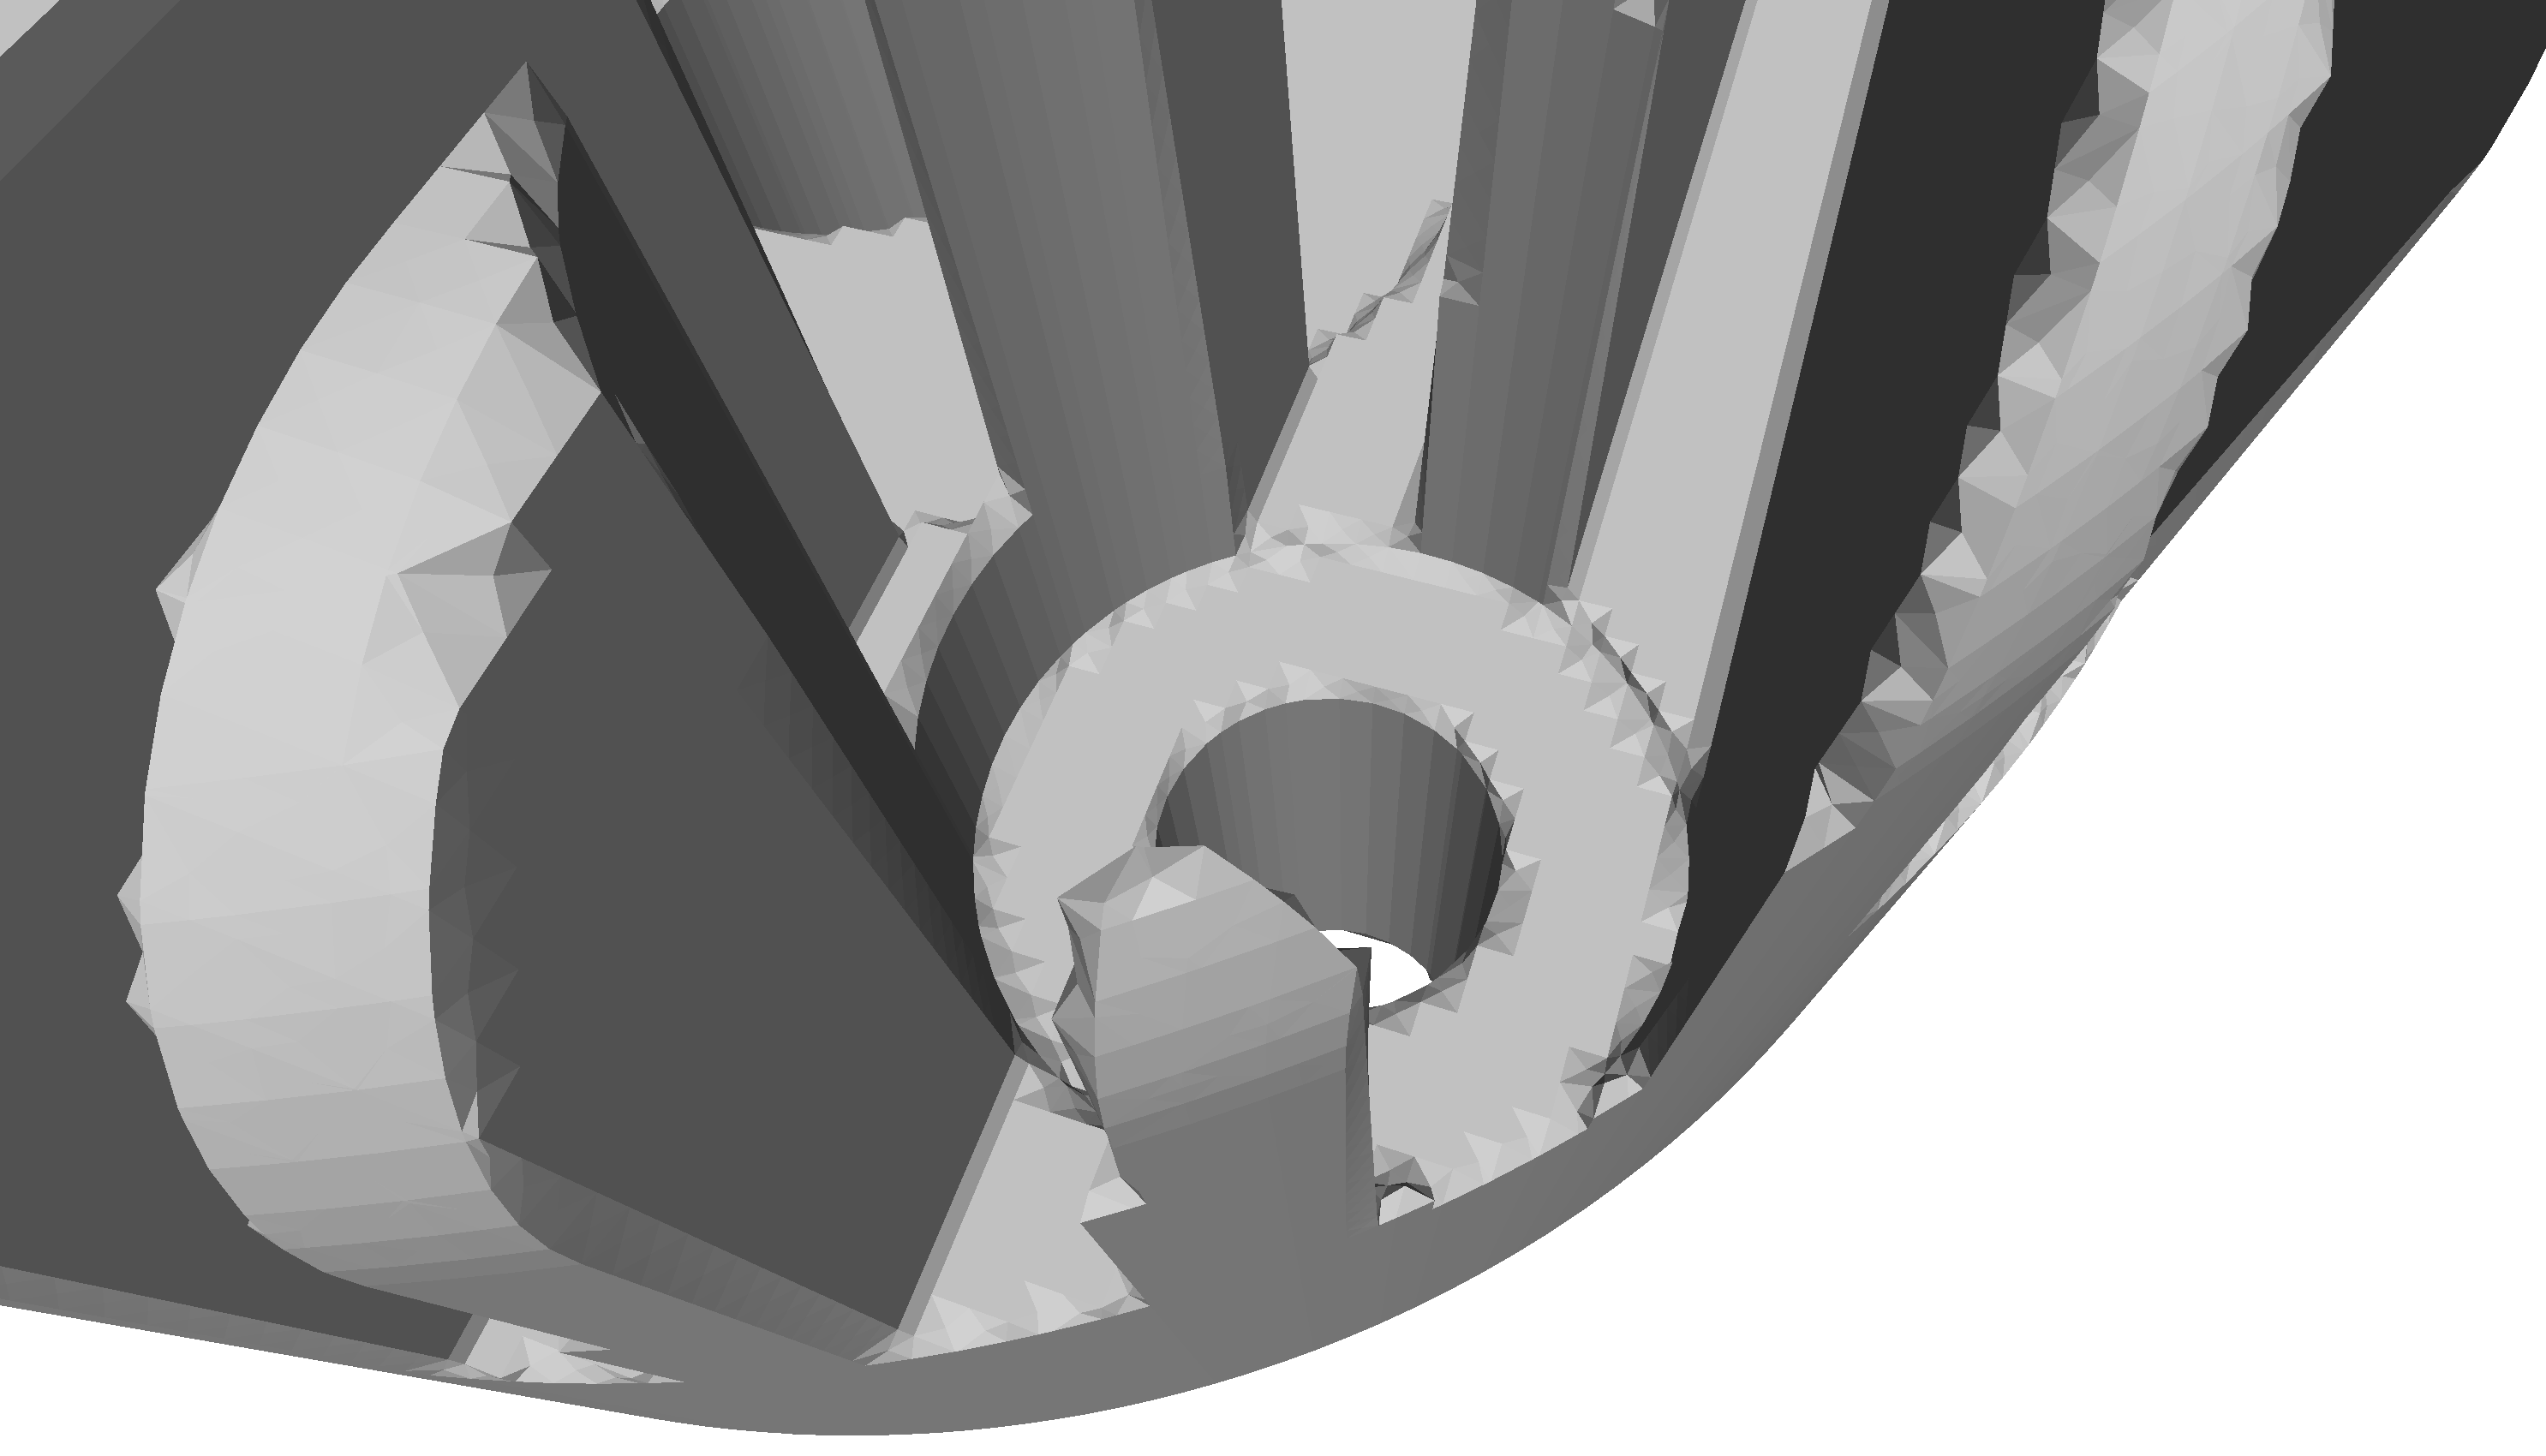
\includegraphics[width=\textwidth]{td_cylinder_head_drilling_no_features}
		\caption{no feature reconstruction}
		\label{fig:td_cylinder_head_drilling_no_features}
	\end{subfigure}
	\bigskip\\
	\begin{subfigure}[b]{0.67\textwidth}
		\centering
		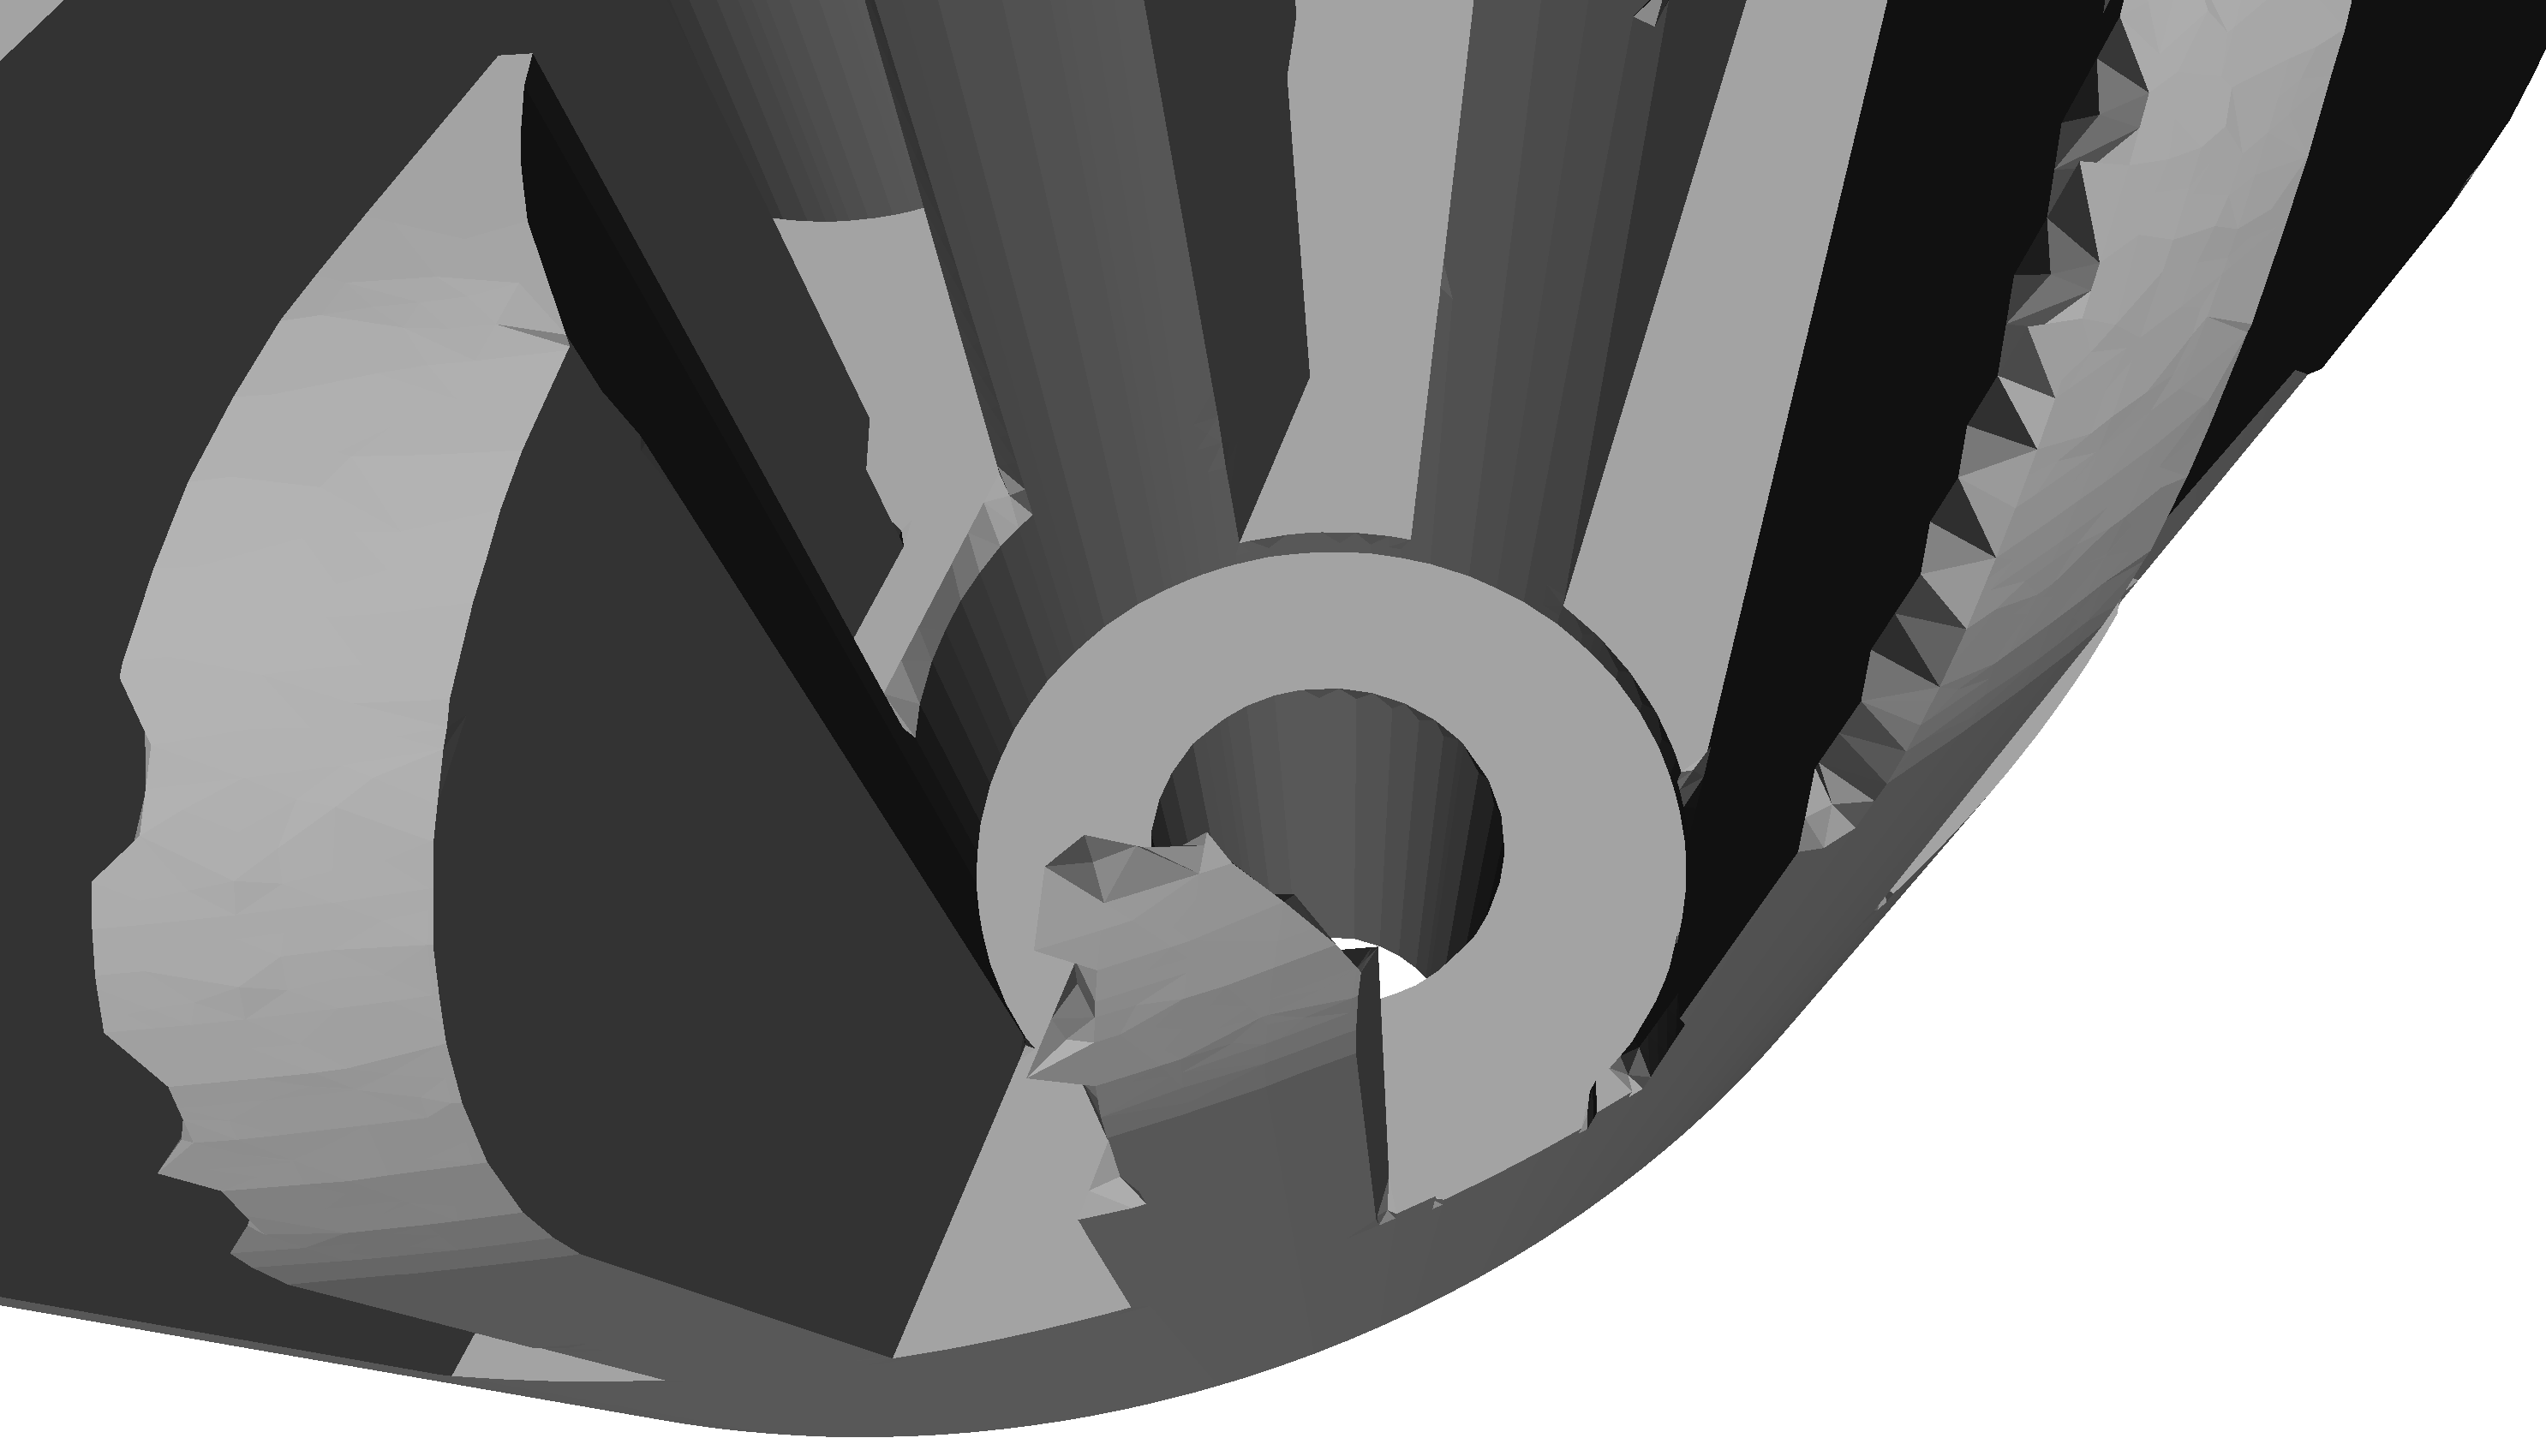
\includegraphics[width=\textwidth]{td_cylinder_head_drilling_features}
		\caption{feature reconstruction}
		\label{fig:td_cylinder_head_drilling_features}
	\end{subfigure}
	\bigskip\\
	\begin{subfigure}[b]{0.67\textwidth}
		\centering
		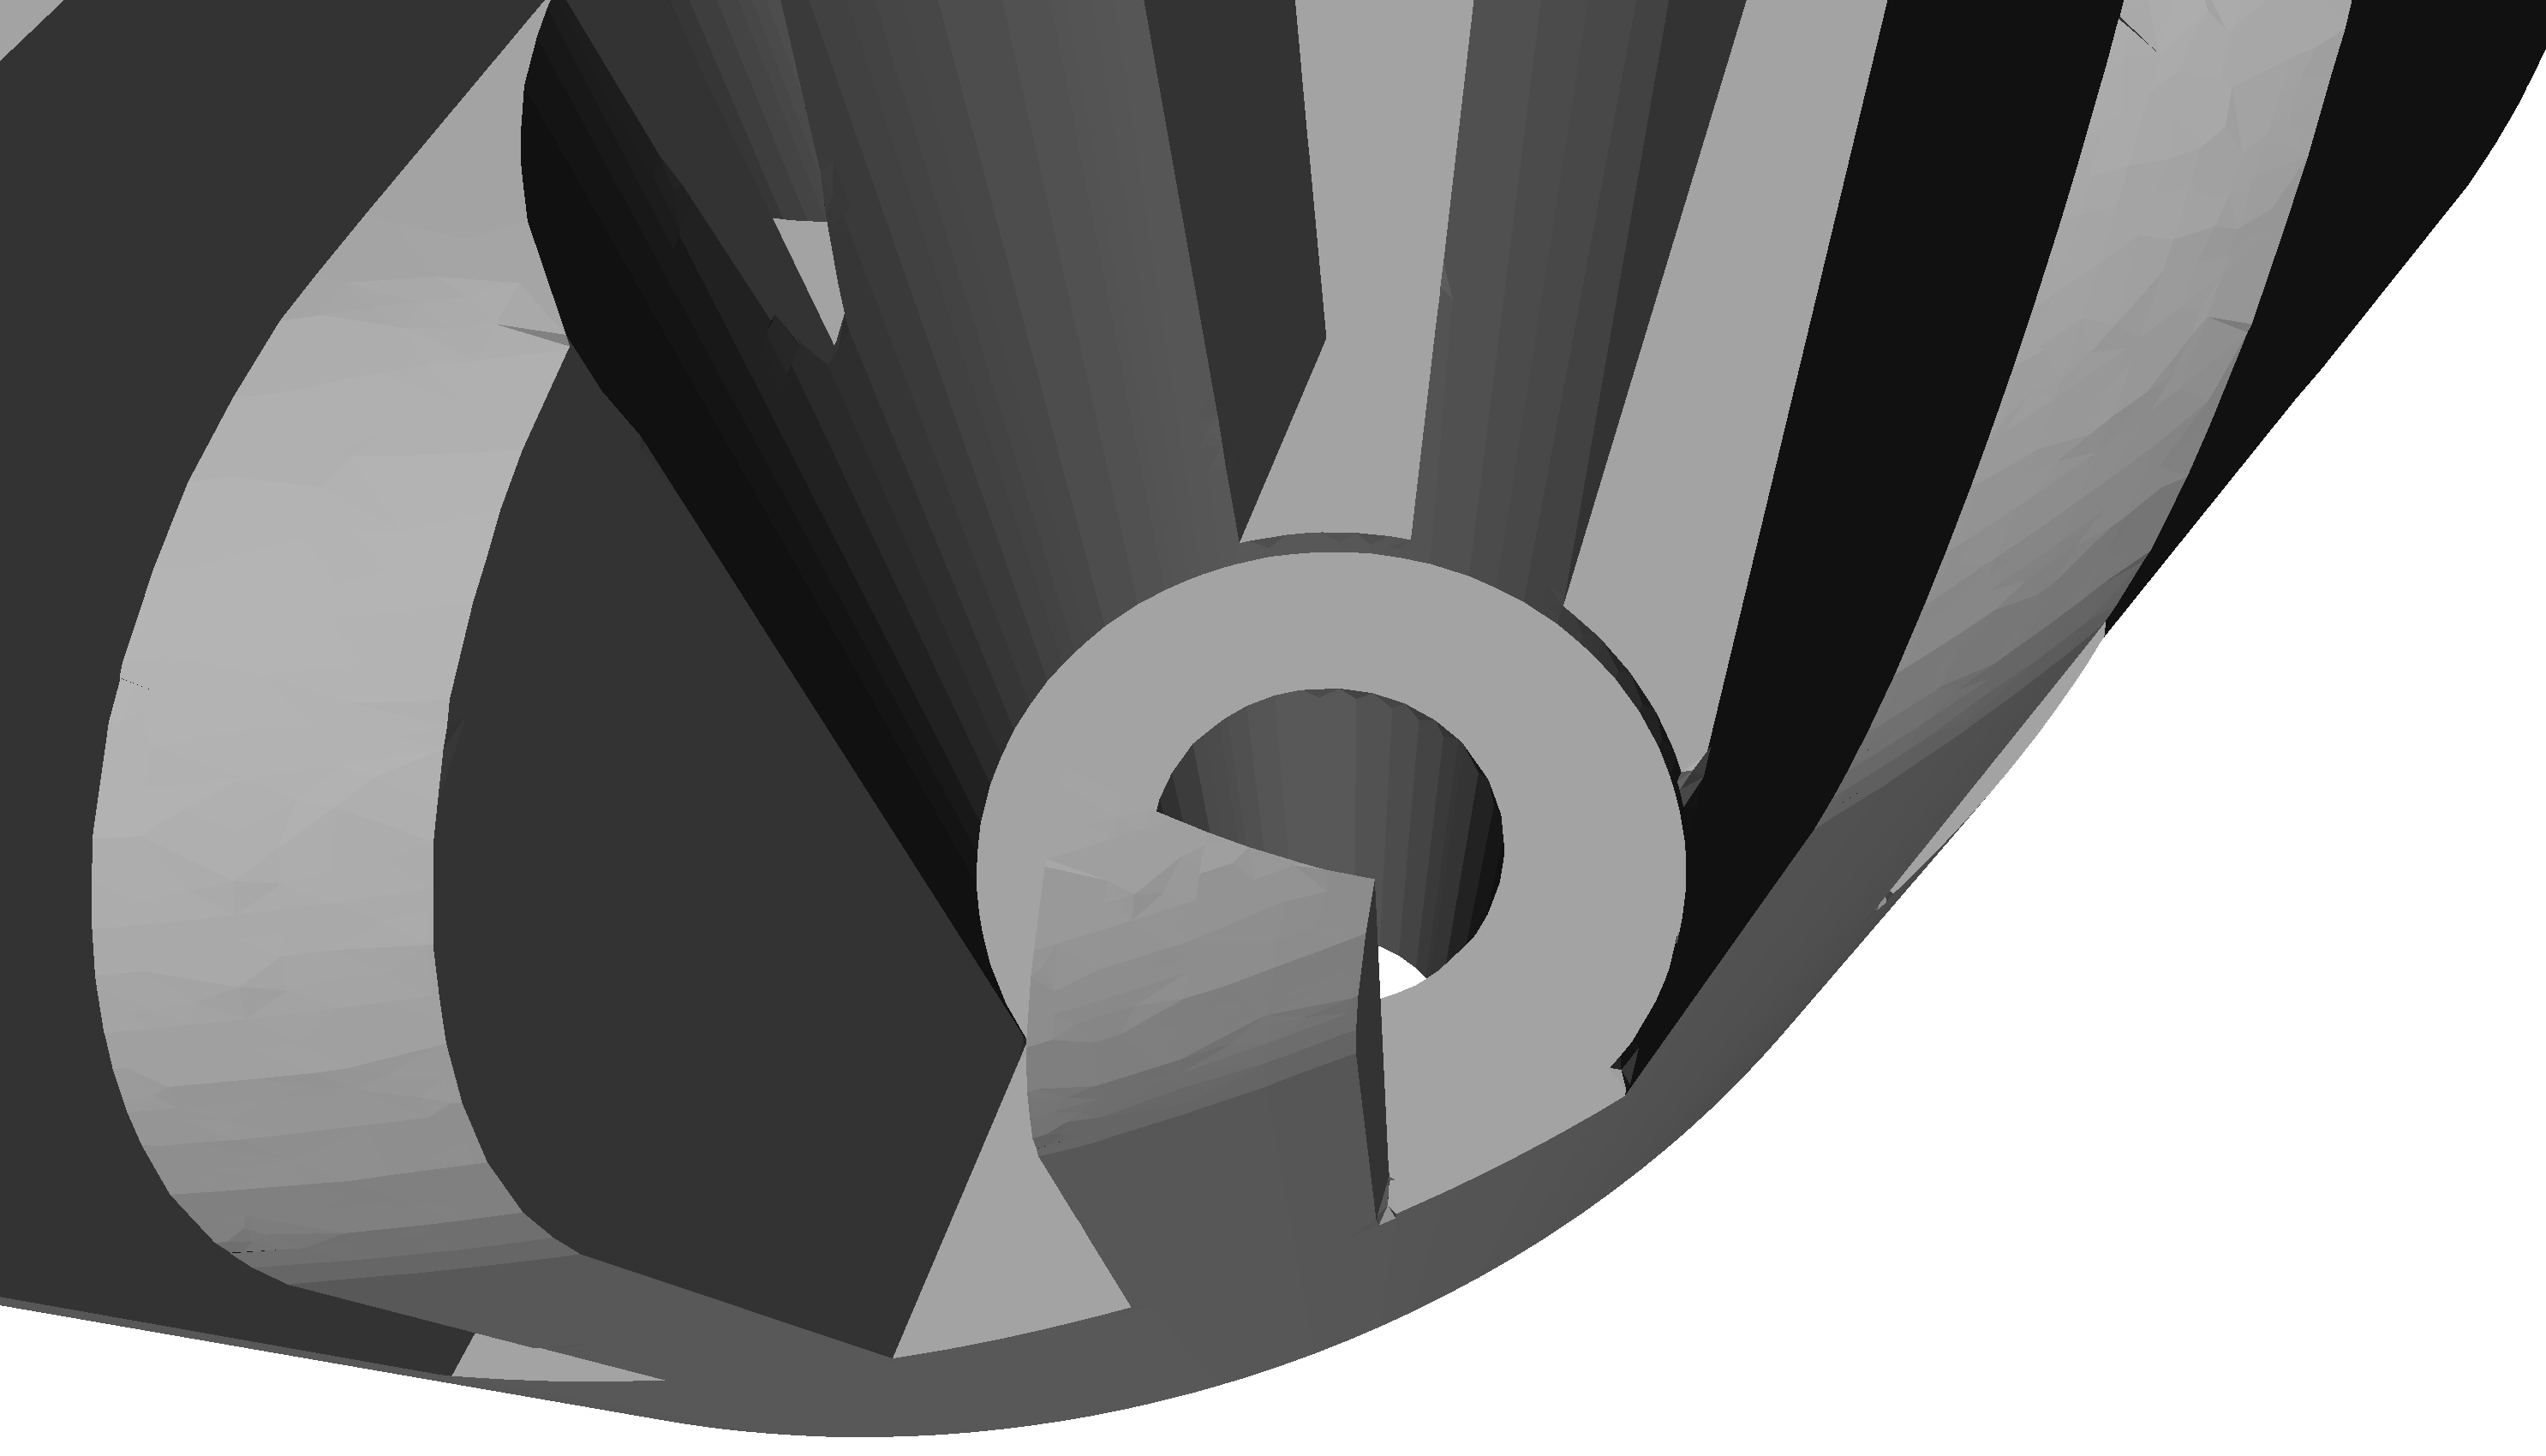
\includegraphics[width=\textwidth]{td_cylinder_head_drilling_cell_slicing}
		\caption{feature reconstruction and cell slicing}
		\label{fig:td_cylinder_head_drilling_cell_slicing}
	\end{subfigure}
	\caption{
		Details of the cylinder\_head scene rendered with the same perspective using MeshLab.
		The renderings show the effects of refinement, feature reconstruction and cell slicing.
		The meshes have been extracted using the tri-dexel approach at a resolution of 100.
	}
	\label{fig:td_features_and_cell_slicing}
\end{figure}
%
Without feature reconstruction, almost no edges are reconstructed correctly.
This is very well observable at drilling and the flat surface around it.
Also the edges of the cylinder\_head's fins lack sharpness.
Enabling feature reconstruction, \cf section \ref{sec:tri_dexel_refinement}, achieves a lot of correctness by using the normal information of the dexel image to calculate good intermediate/feature points and apex vertices.
In addition to the feature reconstruction, the cell slicing strategy, \cf section \ref{sec:tri_dexel_cellslicing}, finally manages to also capture thin features, which were previously thrown away by the regularization.

Although improving the outcome significantly, slicing cells is dangerous.
It may create holes and T-vertices in the mesh, at the border between regular cells and sliced cells, making the mesh orientable but not manifold and closed.
Figure \ref{fig:td_cylinder_head_issues} shows these issues by the example of the outmost rip of the cylinder\_head.
%
\begin{figure}
	\centering
	\begin{subfigure}[b]{0.49\textwidth}
		\centering
		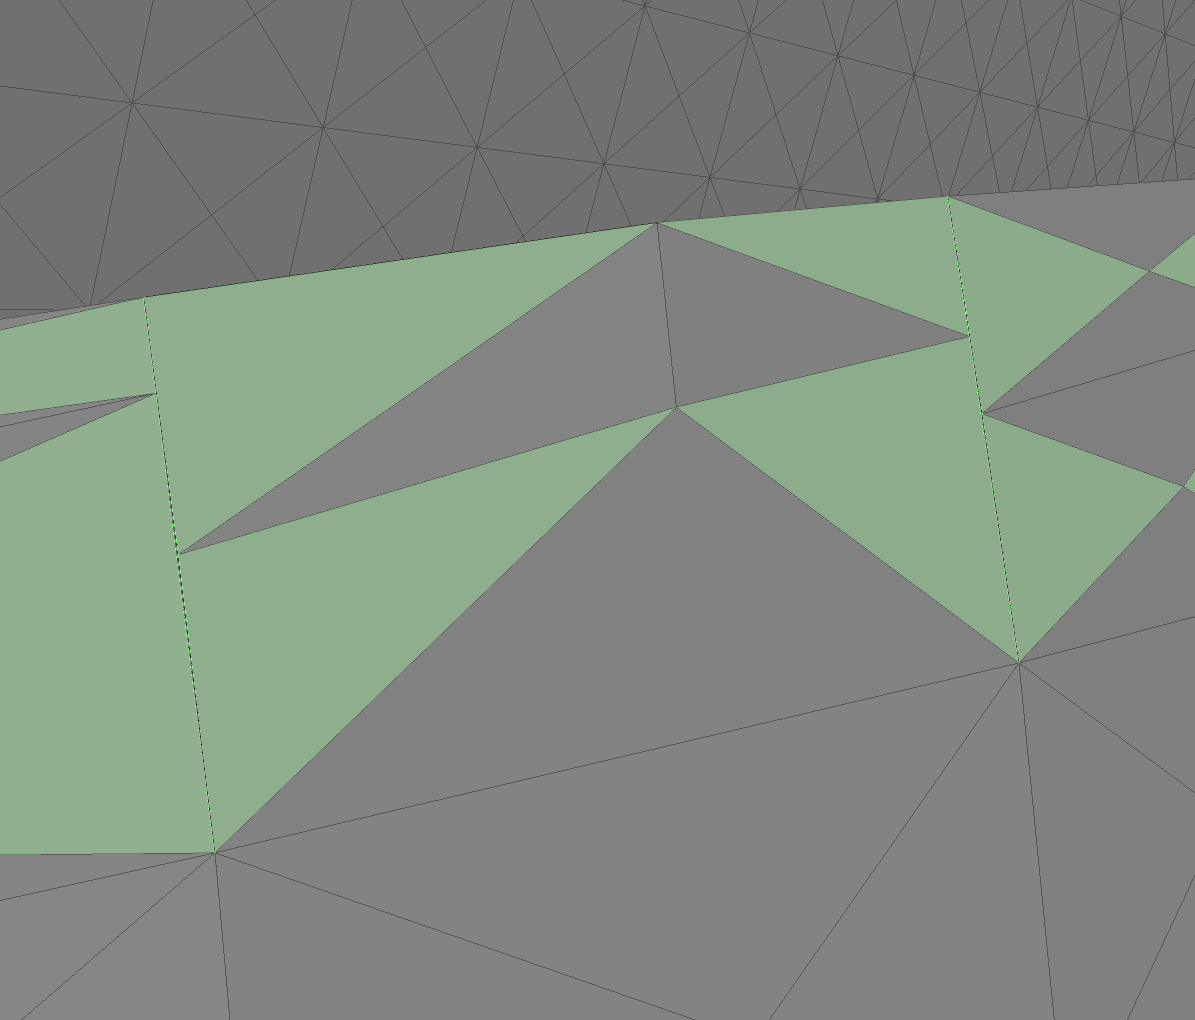
\includegraphics[width=\textwidth]{td_cylinder_head_t_vertex}
		\caption{t-vertices}
		\label{fig:td_cylinder_head_t_vertex}
	\end{subfigure}
	\begin{subfigure}[b]{0.49\textwidth}
		\centering
		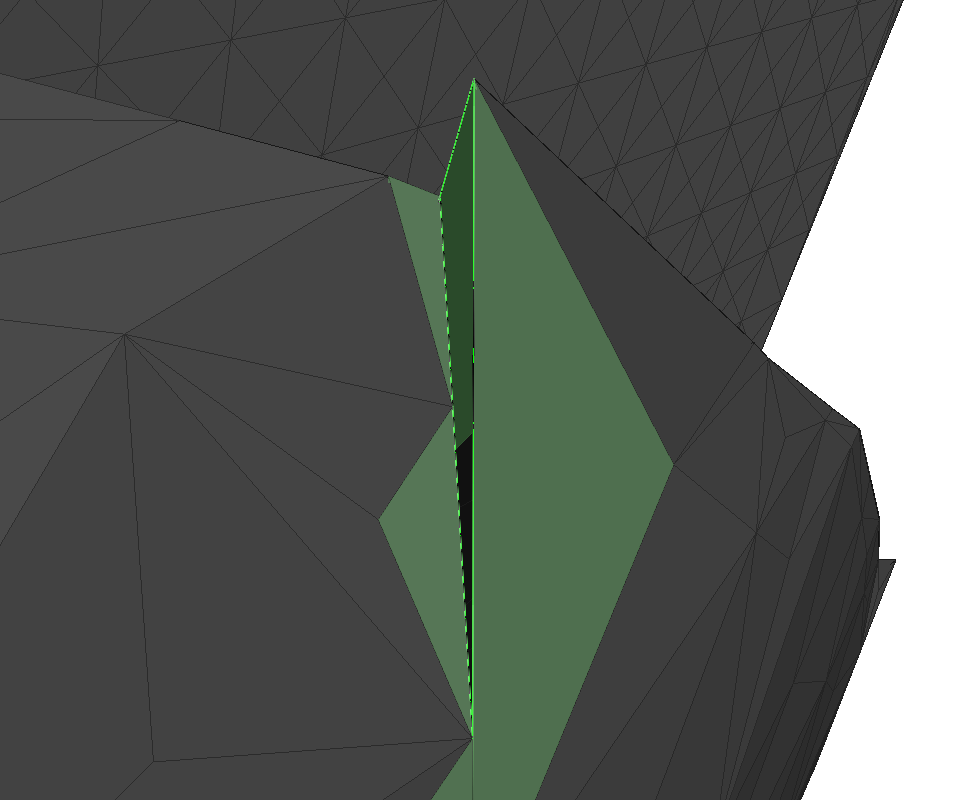
\includegraphics[width=\textwidth]{td_cylinder_head_hole}
		\caption{hole}
		\label{fig:td_cylinder_head_hole}
	\end{subfigure}
	\caption{
		Details of the cylinder\_head scene rendered using MeshLab.
		The renderings show the creation of T-vertices and holes at the border of normal and sliced cells.
		The hole is created at the border of a cell and a sliced cell, which is discussed in figure \ref{fig:tri_dexel_hole_creation}.
		The meshes have been extracted using the tri-dexel approach with cell slicing at a resolution of 100.
	}
	\label{fig:td_cylinder_head_issues}
\end{figure}
%
Still, these holes are usually thin and closable by a post processing step.
If all T-vertices are also fixed, \eg by splitting triangles at the edge spanning the T-vertex, meshes created with cell slicing enabled may still be converted into a manifold and closed result.

Table \ref{tbl:tri_dexel_boundary edges} contains the number of boundary edges for the tested scenes and resolutions and the tri-dexel variant using cell slicing.
%
\begin{table}
\centering
		\begin{tabular}{l|r|r|r|r}
			resolution     &   50 &  100 &  200 &   400 \\
			\midrule
			cube2          &    0 &    0 &    0 &     0 \\
			cylinders\_d   &    0 &  128 &  238 &   846 \\
			cylinders      &    0 &    0 &    0 &     0 \\
			cylinder\_head &  871 & 1880 & 4136 &  4966 \\
			impeller       & 1129 & 2380 & 4654 & 11940 \\
			impeller\_2    &  574 & 1191 & 3033 &  6050 \\
			turbine        & 2006 & 3703 & 7181 & 13803 \\
		\end{tabular}
		\caption{
			Created boundary edges by the tri-dexel surface extraction using cell-slicing and the test scenes described in \ref{tbl:test_scenes}.
			All values were measured using MeshLab.
			The meshes created without cell-slicing do not contain boundary edges.
		}
		\label{tbl:tri_dexel_boundary edges}
\end{table}
%
These numbers are fairly smaller than the ones produced by the direct intersection approach discussed in chapter \ref{ch:direct_intersection}, \cf figure \ref{tbl:direct_intersection_results}.
The cube2 and cylinders scene even contain no boundary edges at all, as no cells have been sliced.
The reason therefore is that the geometry of both scenes is completely convex, resulting in very regular dexel images with long dexels typically spanning the whole workpiece.
The cylinders\_d's triangulation, compared with the cylinders', for example is slightly concave at the lateral surface.
Thus, close rays along these surfaces alternatingly enter and exit the surface, sometimes yielding short dexel segments which lead to irregular edges later.

The more complex scenes produce a larger number of boundary edges, mostly attributed to T-vertices, although the results show, that the number of boundaries is not related to the scene's input triangle or swept volume count, \cf table \ref{tbl:test_scenes}.
The number of boundaries is directly related to the number of irregular cells, which depends on the feature richness, \ie the shape, of the workpiece.
The impeller\_2 scene, for example, contains roughly half as much feature-rich geometry as the impeller scene.
In contrast, the cylinder\_head, despite consisting of two orders of magnitude less swept volumes as the impeller, still produces a third of the impeller's boundary edge count.

Concerning the scenes themselves, the cylinder\_head creates almost all irregular cells and boundaries at the sharp edges of the fins, where subdivision is vital to extract these features.
The impeller scene contains its boundary vertices distributed equally over the machined area.
Finally, the turbine suffers a lot from numerical issues at the rays parallel and to the stock surface which are tinily underneath it, continually entering and exiting the flat surface.
The sliced cells are again irregular and caught by the recursion limit of the cell slicing algorithm.
